\documentclass[12pt,a4paper,oneside,english,spanish]{TesisUNI}

% -----------------------------------
% Configuración de Idioma y Fuente
% -----------------------------------
\usepackage[T1]{fontenc}
\usepackage[spanish, es-tabla]{babel} % Configura el idioma a español y reemplaza "cuadro" por "tabla"
\usepackage{newtxtext} % Utiliza la fuente de texto New Times-like


% -----------------------------------
% Gestión de Bibliografía
% -----------------------------------
\usepackage[style=apa, backend=biber]{biblatex}
\addbibresource{3_3_BIBLIOGRAFIA/library.bib} % Carga la bibliografía desde el archivo 'library.bib'
\usepackage{csquotes} % Mejora la presentación de citas en el texto

\setcounter{tocdepth}{3} % Incluye hasta \paragraph en el índice


% -----------------------------------
% Configuración de Documento
% -----------------------------------
\setcounter{secnumdepth}{3} % Numera hasta las subsubsecciones
\decimalpoint % Utiliza punto decimal en lugar de coma
\usepackage{layouts} % Proporciona herramientas para mostrar el diseño del documento
\usepackage{setspace} % Permite ajustar el espaciado entre líneas
\usepackage[margin=1in]{geometry} % Configura los márgenes del documento
 

% -----------------------------------
% Manejo de Imágenes y Tablas
% -----------------------------------
\usepackage{graphicx} % Permite incluir imágenes
\usepackage{changepage} % Facilita la adición de sangrías
\usepackage{float} % Mejora la colocación de objetos flotantes como imágenes
\usepackage{tabularx} % Permite crear tablas con anchos ajustables


% -----------------------------------
% Configuración de Encabezados y Pies de Página
% -----------------------------------
\usepackage{fancyhdr} % Permite personalizar encabezados y pies de página
\pagestyle{fancy} % Aplica el estilo 'fancy' a las páginas


% -----------------------------------
% Otros Ajustes de Estilo y Formato
% -----------------------------------
\usepackage{lipsum} % Genera texto de relleno
\renewcommand{\labelitemi}{$\bullet$} % Define círculos para las viñetas
\usepackage{titlesec} % Personalización de títulos de secciones
\usepackage{tocloft} % Personalización de índices
\usepackage[colorlinks=true,linkcolor=negro,citecolor=negro]{hyperref} % Configura los enlaces dentro del documento


% -----------------------------------
% Configuración de Matemáticas y Diagramas
% -----------------------------------
\usepackage[mathbf=sym]{unicode-math} % Mantiene las fuentes matemáticas
\usepackage{tikz} % Permite crear gráficos y diagramas
\usetikzlibrary{calc,positioning,shapes.geometric,shapes.symbols,shapes.misc} % Carga bibliotecas adicionales para TikZ

% Definiciones de estilos para los elementos de TikZ
\tikzstyle{startstop} = [rectangle, rounded corners, minimum width=3cm, minimum height=0.5cm,text centered, draw=black]
\tikzstyle{io} = [trapezium, trapezium left angle=70, trapezium right angle=110, minimum width=3cm, minimum height=0.5cm, text centered, text width=3cm, draw=black]
\tikzstyle{process} = [rectangle, minimum width=3cm, minimum height=0.5cm, text centered, text width=4cm, draw=black]
\tikzstyle{decision} = [diamond, minimum width=3cm, minimum height=0.5cm, text centered, draw=black]
\tikzstyle{loop} = [chamfered rectangle,chamfered rectangle xsep=2cm,draw=black]
\tikzstyle{arrow} = [->,>=stealth]
\tikzstyle{line}=[draw]


% -----------------------------------
% Soporte para Código Fuente y Color
% -----------------------------------
\usepackage{listings} % Permite incluir código fuente
\usepackage{color} % Permite definir y utilizar colores

% Definición de nuevos colores
\definecolor{codegreen}{rgb}{0,0.6,0}
\definecolor{codegray}{rgb}{0.5,0.5,0.5}
\definecolor{codepurple}{rgb}{0.2,0,1}
\definecolor{codeRojo}{rgb}{0.7,0,0.3}
\definecolor{backcolour}{rgb}{1.0, 1.0, 1.0}


% -----------------------------------
% Configuraciones Adicionales y Personalizaciones
% -----------------------------------
\usepackage{ragged2e} % Proporciona comandos para alinear texto
\usepackage{booktabs} % Mejora la calidad de las tablas
\usepackage{xstring} % Proporciona funciones avanzadas de manipulación de cadenas
\usepackage{multirow} % Mejora la creación de tablas con celdas que abarcan varias filas
\usepackage{array} % Proporciona funciones adicionales para tablas
\usepackage{subcaption} % Permite el uso de subfiguras y subtítulos
\usepackage{chngcntr} % Permite ajustar la numeración de contadores
\counterwithout{figure}{chapter} % Configura la numeración de figuras independientemente de los capítulos
\makeatletter % Comando para reducir errores


% -----------------------------------
% Configuración de Estilo de Listado de Código
% -----------------------------------
% Definición de estilo personalizado para listados de código
\lstdefinestyle{mystyle}{
  backgroundcolor=\color{backcolour},  
  commentstyle=\color{codegreen},
  keywordstyle=\color{codeRojo},
  numberstyle=\tiny\color{codegray},
  stringstyle=\color{codepurple},
  basicstyle=\footnotesize,
  breakatwhitespace=false,         
  breaklines=true,                 
  captionpos=b,                    
  keepspaces=true,                 
  numbers=left,                    
  numbersep=5pt,                  
  showspaces=false,                
  showstringspaces=false,
  showtabs=false,                  
  tabsize=2
}

\lstset{style=mystyle} % Aplica el estilo 'mystyle' a los listados de código


% -----------------------------------
% Ajustes de Formato de Documento
% -----------------------------------
\newenvironment{MyFont}{\fontfamily{ugm}\selectfont}{\par}
\usepackage{changepage} % Agregar espacio a Listing
\renewcommand{\cfttoctitlefont}{\hfill \normalfont\normalsize\bfseries} % Centrado del título del Índice
\renewcommand{\cftaftertoctitle}{\hfill} % Alineación después del título del Índice
\renewcommand{\cftlottitlefont}{\hfill\normalfont\normalsize\bfseries} % Centrado del título de la Lista de Tablas
\renewcommand{\cftafterlottitle}{\hfill} % Alineación después del título de la Lista de Tablas
\renewcommand{\cftloftitlefont}{\hfill\normalfont\normalsize\bfseries} % Centrado del título de la Lista de Figuras
\renewcommand{\cftafterloftitle}{\hfill} % Alineación después del título de la Lista de Figuras


% ------------------------------------
% Espaciado entre Párrafos y Sangría
% ------------------------------------
\setlength{\parindent}{1.27cm} % Configura la sangría
\doublespacing % Aplica doble espaciado en todo el documento
% \usepackage[section]{placeins}


% ------------------------------------
% Cambio del Título de Bibliografía
% ------------------------------------
\addto\captionsspanish{\renewcommand{\bibname}{\centering Referencias bibliográficas}}


% ------------------------------------
% Posicionamiento Vertical de Índices
% ------------------------------------
% Ajustes para el espacio antes y después de los títulos en el Índice, Lista de Figuras y Lista de Tablas
\setlength{\cftbeforelottitleskip}{1pt} % Espacio antes del título en la Lista de Tablas
\renewcommand{\cftafterlottitleskip}{12pt} % Espacio después del título en la Lista de Tablas
\setlength{\cftbeforeloftitleskip}{1pt} % Espacio antes del título en la Lista de Figuras
\renewcommand{\cftafterloftitleskip}{12pt} % Espacio después del título en la Lista de Figuras
\setlength{\cftbeforetoctitleskip}{16pt} % Espacio antes del título en el Índice
\renewcommand{\cftaftertoctitleskip}{12pt} % Espacio después del título en el Índice


% -------------------------------------
% Configuración de Figuras
% -------------------------------------
% Ajustes de la nomenclatura y formato de las figuras
\addto\captionsspanish{\renewcommand{\figurename}{Figura}} % Cambia el nombre de las figuras a "Figura"
\captionsetup{ % Configuración del formato de las etiquetas para figuras
   justification=raggedright, % Alineación a la izquierda
   singlelinecheck=false, % Aplica justificación incluso para textos cortos
   labelsep=period, % Punto después del número de figura
   labelfont=bf % Texto "Figura Número" en negrita
}

% Comando personalizado para insertar figuras
\newcommand{\insertfigure}[3]{
    \begin{figure}[H] % Usa el entorno 'figure' con opción [H] para ubicación exacta
    \caption{\doublespacing \\ \textit{#1}} % Título de la figura con doble espaciado y en cursiva
    \centering % Centra la imagen
    \includegraphics[width=0.7\linewidth]{#2} % Inserta la imagen
    \begin{justify} % Justifica la descripción
        \textit{Nota.} #3 % Descripción o nota asociada a la figura
    \end{justify}
    \label{fig:#1} % Etiqueta para referencia cruzada
    \end{figure}
}


% -------------------------------------
% Configuración de Tablas
% -------------------------------------
\counterwithout{table}{chapter} % Configura la numeración de tablas independiente de capítulos
\addto\captionsspanish{\renewcommand{\tablename}{Tabla}} % Cambia el nombre de las tablas a "Tabla"
\captionsetup[table]{ % Configuración del formato de las etiquetas para tablas
   justification=raggedright, % Alineación a la izquierda
   singlelinecheck=false, % Aplica justificación incluso para textos cortos
   labelsep=period, % Punto después del número de tabla
   labelfont=bf % Texto "Tabla Número" en negrita
}

\newcolumntype{P}[1]{>{\justifying\noindent\arraybackslash}p{#1}} % Nuevo tipo de columna para tablas

% Define que las tablas sean numeradas con números arábigos
\renewcommand{\thetable}{\arabic{table}}  


% -------------------------------------
% Espaciamiento y Nomenclatura en Índices
% -------------------------------------
% Ajustes para el espaciamiento y la nomenclatura en el Índice, Lista de Figuras y Lista de Tablas
\setlength{\cftbeforechapskip}{2mm} % Espaciado antes de capítulos en el Índice
\renewcommand\cftchapafterpnum{\vskip6pt} % Espaciado después de capítulos en el Índice
\renewcommand\cftsecafterpnum{\vskip5pt} % Espaciado después de secciones en el Índice
\renewcommand\cftsubsecafterpnum{\vskip5pt} % Espaciado después de subsecciones en el Índice

\renewcommand{\cftchappresnum}{} % Elimina cualquier prefijo para el número del capítulo
\renewcommand{\cftchapaftersnum}{. } % Añade un punto y un espacio después del número del capítulo
\renewcommand{\cftfigpresnum}{Figura N° } % Prefijo "Figura N°" en la Lista de Figuras
\renewcommand{\cftfigaftersnum}{.} % Separador después del número de figura
\renewcommand{\cftfignumwidth}{6.85 em} % Ancho para el número de figura
\renewcommand{\cfttabpresnum}{Tabla N° } % Prefijo "Tabla N°" en la Lista de Tablas
\renewcommand{\cfttabnumwidth}{6.5 em} % Ancho para el número de tabla


% ------------------------------------
% Cambios en la Numeración de Capítulos
% ------------------------------------
% Cambia el formato de numeración de capítulos a números árabes
\renewcommand{\thechapter}{\arabic{chapter}}

% Cambia el formato de numeración de ecuaciones para incluir el número de capítulo
\renewcommand{\theequation}{\arabic{chapter}.\arabic{equation}} 

% Cambia el formato de numeración de secciones para incluir el número de capítulo
\renewcommand{\thesection}{\arabic{chapter}.\arabic{section}} 


% --------------------------
% Nuevo Contador para Capítulos Especiales
% --------------------------
\newcounter{ChapterRoman}
\renewcommand{\theChapterRoman}{\Roman{ChapterRoman}}


% -----------------------------------
% Configuración de Capítulos Especiales
% -----------------------------------
\newcommand{\Chapter}[1]{
    \clearpage % Asegura que empezamos en una página nueva
    \refstepcounter{ChapterRoman} % Incrementa el contador
    \thispagestyle{empty} % Elimina encabezados y pie de página para esta página
    \null\vfill % Centra el contenido verticalmente
    \begin{center} % Centra el contenido horizontalmente
        \Large\bfseries CAPÍTULO \theChapterRoman\ \\[1em] #1 % Título del capítulo
    \end{center}
    \vfill\null % Centra el contenido verticalmente
    % \addcontentsline{toc}{chapter}{CAPÍTULO \theChapterRoman: #1} % Agrega la entrada al Índice
    \addcontentsline{toc}{chapter}{CAPÍTULO \theChapterRoman} % Elimina ': #1' para quitar el título
    \clearpage % Comienza una nueva página después del título del capítulo
}


% -----------------------------------
% Formateo de Encabezados de Sección
% -----------------------------------
% Nivel 1 (\chapter)
% Para los títulos de capítulos en el cuerpo del documento
\titleformat{\chapter}[block]
  {\normalfont\normalsize\bfseries\centering}
  {\thechapter.} % Elimina el punto si no quieres el número de capítulo seguido de un punto
  {0.5em}
  {\MakeUppercase}
\titlespacing*{\chapter}{0pt}{12pt}{5pt} % Espaciado para \chapter

% Nivel 2 (\section)
\titleformat{\section}[block]
  {\normalfont\normalsize\bfseries\raggedright}
  {\thesection}
  {0.5em}
  {}
\titlespacing*{\section}{0pt}{12pt}{5pt} % Espaciado para \section

% Nivel 3 (\subsection)
\titleformat{\subsection}[block]
  {\normalfont\normalsize\bfseries\itshape\raggedright}
  {\thesubsection}
  {0.5em}
  {}
\titlespacing*{\subsection}{0pt}{12pt}{5pt} % Espaciado para \subsection

% Nivel 4 (\subsubsection)
\titleformat{\subsubsection}[runin]
  {\normalfont\normalsize\bfseries\raggedright}
  {\thesubsubsection}
  {0.5em}
  {}[. \quad]
\titlespacing*{\subsubsection}{1.27cm}{12pt}{0pt} % Espaciado para \subsubsection

% Nivel 5 (\paragraph)
\titleformat{\paragraph}[runin]
  {\normalfont\normalsize\bfseries\itshape\raggedright}
  {\theparagraph}
  {0.5em}
  {}[. \quad]
\titlespacing*{\paragraph}{1.27cm}{12pt}{0pt} % Espaciado para \paragraph


% -------------------------------------
% Definición de Colores
% -------------------------------------
\usepackage{xcolor} % Importación del paquete de colores
\definecolor{granate}{RGB}{113,22,16} % Define el color granate
\definecolor{gris}{RGB}{154,153,157} % Define el color gris
\definecolor{arena}{RGB}{230,217,170} % Define el color arena
\definecolor{azul}{rgb}{0.03, 0.15, 0.4} % Define el color azul
\definecolor{negro}{rgb}{0, 0, 0} % Define el color negro


% -------------------------------------
% Configuración de Listado de Código
% -------------------------------------
\lstset{ % Configuración para listados de código
  language=Python, % Lenguaje de programación
  basicstyle=\ttfamily\small, % Estilo básico
  commentstyle=\color{gray}, % Estilo para comentarios
  keywordstyle=\color{blue}, % Estilo para palabras clave
  stringstyle=\color{red}, % Estilo para cadenas de texto
  numberstyle=\tiny\color{gray}, % Estilo para números de línea
  numbers=left, % Posición de números de línea
  stepnumber=1, % Intervalo de números de línea
  showstringspaces=false, % No mostrar espacios en cadenas
  tabsize=4, % Tamaño de tabulación
  breaklines=true, % Romper líneas largas
  frame=single, % Marco alrededor del código
  literate=% Configuración para caracteres especiales
  {á}{{\'a}}1 {é}{{\'e}}1 {í}{{\'i}}1 {ó}{{\'o}}1 {ú}{{\'u}}1
  {Á}{{\'A}}1 {É}{{\'E}}1 {Í}{{\'I}}1 {Ó}{{\'O}}1 {Ú}{{\'U}}1
  {ñ}{{\~n}}1 {Ñ}{{\~N}}1 {ü}{{\"u}}1 {Ü}{{\"U}}1
}

\begin{document}
	\creaportada
	\renewcommand\contentsname{\centering TABLE OF CONTENTS }
	\tableofcontents	
	
	% \cleardoublepage\phantomsection\addcontentsline{toc}{chapter}{\bf RESUMEN}
\chapter*{\centerline {RESUMEN}}
\markboth{RESUMEN}{}

\lipsum[5] 


		
	% \cleardoublepage\phantomsection\addcontentsline{toc}{chapter}{\bf {ABSTRACT}}
\chapter*{\centerline {ABSTRACT}}
\markboth{ABSTRACT}{}

\lipsum[5]

	% \cleardoublepage\phantomsection\addcontentsline{toc}{chapter}{\bf {PRÓLOGO}}
\chapter*{\centerline {PRÓLOGO}}
\markboth{PRÓLOGO}{}

\lipsum[6] \\ [2mm]
\lipsum[10] 

 
	
	
	%Cambiar nombre, crear ÍNDICE DE FIGURAS Y TABLAS
	
	\renewcommand\listfigurename{\centering LISTA DE FIGURAS}
	\renewcommand\listtablename{\centering LISTA DE TABLAS}

	% \cleardoublepage\phantomsection\addcontentsline{toc}{chapter}{\listtablename}
	% {\normalsize\listoftables}
		
	% \cleardoublepage\phantomsection\addcontentsline{toc}{chapter}{\listfigurename}
	% {\normalsize\listoffigures}
	
	% \cleardoublepage\phantomsection\addcontentsline{toc}{chapter}{LISTA DE SÍMBOLOS Y SIGLAS}	
\chapter*{\centerline {LISTA DE SÍMBOLOS Y SIGLAS}}
\markboth{LISTA DE SÍMBOLOS Y SIGLAS}{}
%---
	\section*{\textbf{\underline{SÍMBOLOS}}}

\begin{tabular}{L{0.5 cm}p{0.025 cm}p{12.5 cm}}
$\alpha$           & : & Razón entre la rigidez postfluencia y la   rigidez elástica \\
$A$                & : & Área de la sección transversal de la viga                                                  \\
$\beta$            & : & Porcentaje de amortiguamiento crítico de la superestructura                                \\
$\beta_{a}$        & : & Fracción de amortiguamiento crítico del AMS                                                \\
$\beta_{M}$        & : & Amortiguamiento efectivo de la edificación aislada                                         \\
$B_{M}$            & : & Factor de reducción asociado al amortiguamiento efectivo   $\beta_{M}$                     \\
$c_{a}$            & : & Amortiguamiento del AMS                                                                     
\end{tabular}






	\newpage
	\section*{\textbf{\underline{SIGLAS}}}

\begin{tabular}{L{1.0 cm}p{0.025 cm}p{11.7 cm}}
ADAS    & : & Added damping and stiffness                                                    \\
AMS     & : & Amortiguador de masa sintonizada                                               \\
AS      & : & Aislador sísmico                                                               \\
ASCE    & : & American society of civil engineers                                            
\end{tabular}\\




 
 
	% %Parte CENTRAL DE LA TESIS
	
	\mainmatter 

	\chapter{Introduction}

As the world becomes increasingly interconnected, the ability to observe and analyze our environment from space has emerged as one of the most important tools in addressing global challenges. From this perspective, satellite missions, through their advanced sensor systems, allow the collection of information about the Earth's surface, providing the most detailed and extensive view of the processes of change on our planet. Among the key disciplines that enable these functions, remote sensing stands out, transforming the data obtained by these sensors into critical information for solving environmental and social issues. This discipline provides specific analyses of the transformations and characteristics of certain geographic areas. With advancements in AI (Artificial Intelligence), analytical capabilities have reached a new level, allowing almost any type of satellite image to be analyzed with unprecedented precision and efficiency.

Spatial resolution is a fundamental parameter for the analysis of remote sensing images. It is defined as the minimum ground distance that separates two independent objects that can be distinguished. The factors that determine it include altitude, distance, and the quality of the instruments used \autocite{alparone2015remote}. Another important factor related to spatial resolution is Ground Sampling Distance (GSD), which is the portion of the Earth's surface represented by each pixel \autocite{lillesand2015remote}.

One of the most widely used sensors due to its high spatial resolution is the Sentinel-2 MSI, operated by the European Space Agency \autocite{Sentinel2_Handbook}. Since its launch in June 2015, it has provided open-access multispectral images, generating significant interest in the scientific community and various industries, becoming a key tool for providing data in applications such as land use monitoring, change detection, and vegetation analysis. The sensor is equipped with 13 spectral bands distributed in three spatial resolutions: 4 spectral bands with a resolution of 10 m, 6 spectral bands with 20 m, and 3 spectral bands with 60 m, designed for the collection of various topographic parameters \autocite{lanaras2018super}. This spectral diversity enables detailed studies on a wide range of terrestrial phenomena by combining specific bands, from water quality assessment to snow surface monitoring.

Another sensor that stands out for its higher resolution is the National Agriculture Imagery Program (NAIP), which provides aerial images with a resolution of up to 1 meter. Although its coverage is limited to the continental United States, it offers aerial images with a spatial resolution of up to 1 meter, making it an important source for studies requiring a higher level of detail. NAIP captures images during the peak agricultural activity months, from June to August, and provides updates every three years (previously every five years before 2009). Since 2011, the images have consistently included RGB and NIR bands, improving their quality and applicability in areas such as urban planning and agricultural monitoring. Although NAIP and Sentinel-2 have different approaches and scopes, the combination of images from both sensors allows for a greater richness of data, which is crucial for studies requiring both extensive coverage and exceptional detail.

There are various techniques to address the limitation of spatial and spectral resolution in satellite images within the field of remote sensing, from traditional image fusion methods to more recent approaches based on artificial intelligence. Among the latter, deep learning has proven to be especially promising \autocite{gargiulo2019fast}. One of the most effective applications of this technique is super-resolution, which seeks to increase the spatial resolution of images by generating additional details from existing data. These machine learning techniques allow for the reconstruction of higher-resolution images from lower-quality versions, optimizing both spatial precision and spectral coherence.

\section{Motivation}

The development of techniques to improve the resolution of images obtained by the Sentinel-2 sensor has been a significant challenge in the scientific community. In this process, advanced deep learning architectures such as Generative Adversarial Networks (GANs) and Convolutional Neural Networks (CNNs) play a crucial role, efficiently managing the data \autocite{salgueiro2020super}. Achieving an increase in spatial resolution while maintaining spectral coherence and optimizing data quality opens new frontiers in satellite image analysis.

The availability of free and high-quality images, such as those provided by Sentinel-2, is a valuable resource for scientific research. Although there are other ways to obtain high-resolution images, they often do not cover as large areas or have the necessary temporal resolution for certain studies. Thanks to its global coverage and high revisit frequency, this sensor offers a significant advantage in this regard. Improving its resolution would allow for more detailed studies without the need to resort to costly sensors, making the available data even more impactful.

Additionally, this work seeks to contribute to the advancement of AI in remote sensing applications. By using innovative architectures, this research has the potential to open new possibilities for improving satellite image resolution. This approach not only benefits current science but also has the potential to inspire future research, allowing the continued development of these techniques in new contexts.

\section{Problem Statement}

Despite the availability of advanced super-resolution models \autocite{salgueiro2020super, navarro_sánchez_2020}, the main challenge lies in ensuring that the resulting images not only improve spatial resolution but also maintain spectral coherence, a crucial factor in scientific applications. To overcome the spatial resolution limitations of sensors like Sentinel-2, this work proposes the use of advanced super-resolution techniques based on deep learning models. Super-resolution has become a powerful tool for enhancing image quality, using architectures such as Convolutional Neural Networks (CNNs) and Generative Adversarial Networks (GANs) to generate high-resolution images while preserving spectral and spatial coherence. These techniques, applied to Sentinel-2 multispectral images, have the potential to produce results comparable to those obtained with higher-resolution sensors like NAIP, but with the advantage of working with more accessible data.

In various studies, the Wald Protocol has been followed, a standard in the field of remote sensing, to validate the quality of super-resolved images. This protocol establishes rigorous criteria that ensure the enhanced images maintain spectral and spatial consistency with the original images. In this work, a super-resolution (SR) model is proposed that transforms the 10m and 20m bands of Sentinel-2 into higher-resolution images (2.5m), preserving critical spectral details for precise studies. The enhancement process includes an intermediate step of super-resolution from 10m to 40m, which strengthens the model's robustness.

Furthermore, the use of the Wald Protocol ensures that the fused images retain both spatial and spectral integrity, validating their quality. This approach, which separates the image fusion and resolution enhancement processes through super-resolution, allows each stage to work independently, increasing the versatility and applicability of the proposed method for different types of sensors and applications.

This research not only aims to advance the field of image super-resolution but also offers a viable and accessible solution for projects that require high-resolution images but must operate within the economic and technical limitations of current sensors.

\section{Structure of the Work}

In \textbf{Chapter One}, the purpose and motivation of the work are established. The problem addressed focuses on the need to improve the spatial resolution of satellite images, specifically those from Sentinel-2, through super-resolution techniques. The chapter also describes the organization of the thesis, outlining the main sections and objectives.

\textbf{Chapter Two} delves into a detailed analysis of the context, examining the current state of satellite imaging technologies and the demand for high-resolution data in various fields, such as environmental monitoring and urban planning. The benefits and challenges of improving spatial resolution through multispectral data fusion and super-resolution models are discussed, with a focus on the limitations of existing techniques.

\textbf{Chapter Three} reviews the state of the art in super-resolution technologies applied to satellite images. The chapter provides an overview of key methods such as pansharpening, image model inversion, and deep learning approaches. It also highlights the importance of the Wald Protocol as a validation framework to ensure spectral and spatial consistency in the generated high-resolution images.

In \textbf{Chapter Four}, the general and specific objectives of the project are defined. The main objective is to develop a super-resolution model capable of improving Sentinel-2 images from 10m and 20m resolution to 2.5m resolution using a combination of Convolutional Neural Network (CNN) models and multispectral data fusion techniques. The methodology section details the process followed for model training, dataset preparation, and evaluation using the Wald Protocol.

\textbf{Chapter Five} presents the functional and non-functional requirements of the super-resolution system. Functional requirements include the ability to handle multispectral images of various resolutions and generate consistent, high-quality results with a resolution of 2.5m. Non-functional requirements focus on the system's efficiency, scalability, and robustness in handling large datasets.

In \textbf{Chapter Six}, the development of the super-resolution model is explained in detail. This includes the training process, the design of the neural network architectures (Fusion X2 and X4 models), and the integration of deep learning techniques. The limitations encountered during the training phase, such as memory constraints and model performance, are discussed along with potential optimizations.

\textbf{Chapter Seven} evaluates the performance of the developed model, comparing it with existing techniques. The evaluation is based on both qualitative and quantitative metrics, focusing on the spatial and spectral fidelity of the generated high-resolution images. The chapter also includes an analysis of the system's usability and its potential impact on real-world applications, such as precision agriculture and land use monitoring.

\textbf{Chapter Eight} concludes the work by summarizing the main contributions of the thesis and proposing future research directions. Possible improvements include refining the deep learning architecture, exploring other fusion techniques, and applying the model to different types of satellite images.

\textbf{Appendix I} includes output images generated by the super-resolution model, demonstrating the improved resolution for various Sentinel-2 bands.

\textbf{Appendix II} presents the results of the Wald Protocol validation tests, showing the system's performance in maintaining spectral and spatial consistency.

\textbf{Appendix III} provides detailed documentation of the software tools and libraries used for the model's implementation.

\textbf{Appendix IV} contains the research paper associated with this thesis, submitted for publication.

	\chapter{Context analysis}

\section{Datasets}
\label{chapter:datasets}
In the realm of super-resolution algorithms, the choice of the dataset can significantly influence the algorithm's training and ultimately its performance. Three key datasets in this domain are the OpenImage Dataset, the WorldStrat Dataset, and the Sen2Venus Dataset. Upon contrasting these datasets, it becomes evident that there are several trade-offs to consider. These trade-offs, depending on the nature of the super-resolution tasks to be performed, could significantly influence the choice of the dataset. The OpenImage Dataset, for instance, excels with its $HR$ image pairs that reach up to 0.5 meters. However, its $LR$ pairs are synthetically generated and are geographically limited to the United States. Consequently, its global applicability may be limited, which could potentially constrain its utility in worldwide scenarios. The WorldStrat dataset, on the other hand, stands out with its diversity, offering a wide range of scenes and landscapes. This diverse sampling can enhance the generalization capabilities of SR algorithms. However, its approach of not filtering low-resolution revisits by their cloud coverage introduces an additional layer of complexity. Additionally, it is quite small in comparison to the size if the models. Lastly, the Sen2Venus Dataset is noted for its well-managed pre-processing that assures good correspondence between $LR$ and $HR$ images in the spectral domain. However, the $HR$ image has only double the spatial resolution of the $LR$ image and may lack the diversity found in the WorldStrat dataset. Below, we provide a more detailed explanation of each dataset.

\subsection{OpenImages}
OpenImages is a popular computer vision dataset that provides a large collection of labeled images for training and evaluating machine learning models. The dataset covers a wide range of visual concepts and objects, including people, cars, houses, trains, animals, etc.  It is widely used in tasks such as object detection, image classification, and visual relationship detection. For SR purposes, the amount and quality of the annotations are not of importance, but rather that it is an easily accessible and freely available dataset (CC-BY) containing over  millions images. The original authors of the latent-diffusion model used this dataset to train their checkpoints.

Since it is a computer vision dataset, it only contains RGB images of every-day scenes taken with standard digital cameras. Not only are therefore the objects depicted in the images completely unrelated to the remote sensing domain, their spectral characteristics are vastly different as well. In order to train 4 band models, a 4th band is artificially created from the image intensity and appended in the band dimension. The $LR$ image is created by interpolating the $HR$ version to the desired size of $128x128$ pixels.

The data in question is not directly connected to the research problem in terms of its spectral, spatial, or domain characteristics. However, the large volume of images proves valuable for training a freshly initialized model on fundamental image attributes and connections. Surprisingly, when applying super-resolution techniques to remote sensing imagery using autoencoders and denoising U-Nets trained on the OpenImages dataset, remarkably good results have been achieved. This demonstrates that the knowledge acquired through training on the OpenImages dataset can be transferred to the remote sensing domain and create a solid base for finetuning on more sophisticated datasets.

\begin{figure}[H] 
    \caption{\doublespacing \\ \textit{Example of an OpenImages LR and HR image pair.}} 
    \centering
    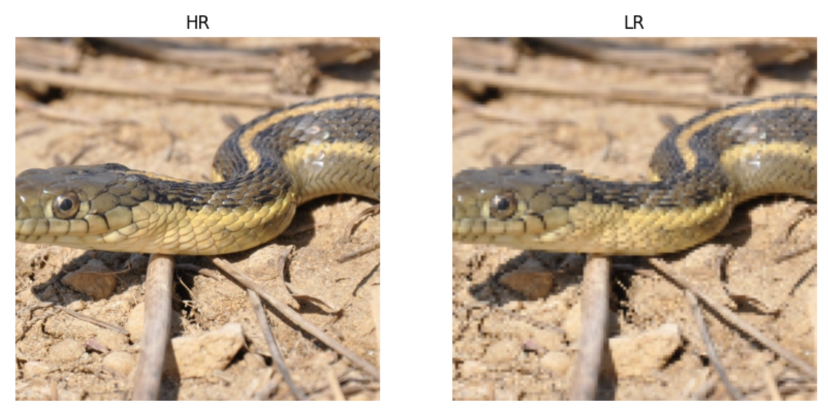
\includegraphics[width=1\linewidth]{images/openimages_example.png}
    \begin{justify}
        \textit{Note.} Example of an OpenImages LR and HR image pair.
    \end{justify}                    
    \label{fig:openimages_example}
\end{figure}

\subsection{Sentinel-2 Dataset}


\subsection{NAIP Dataset}
The National Agriculture Imagery Program (NAIP) acquires high-resolution aerial imagery of agricultural areas in the United States. It provides current and accurate imagery to support agricultural applications and decision-making. NAIP captures imagery at a spatial resolution of 0.6 meters, allowing for detailed analysis of agricultural activities. Using specialized aerial platforms with multispectral sensors, NAIP collects data in various spectral bands, including red, green, blue, and near-infrared. The NAIP dataset covers diverse agricultural regions and is regularly updated. It is freely available to the public, facilitating its use in agricultural research, precision farming, land management, and related applications. A comparison between Sentinel-2 and NAIP is shown in Figure \ref{fig:naip_comparison}.

\begin{figure}[H] 
    \caption{\doublespacing \\ \textit{Comparison between Sentinel-2 and NAIP near Rapid City, South Dakota.}} 
    \centering
    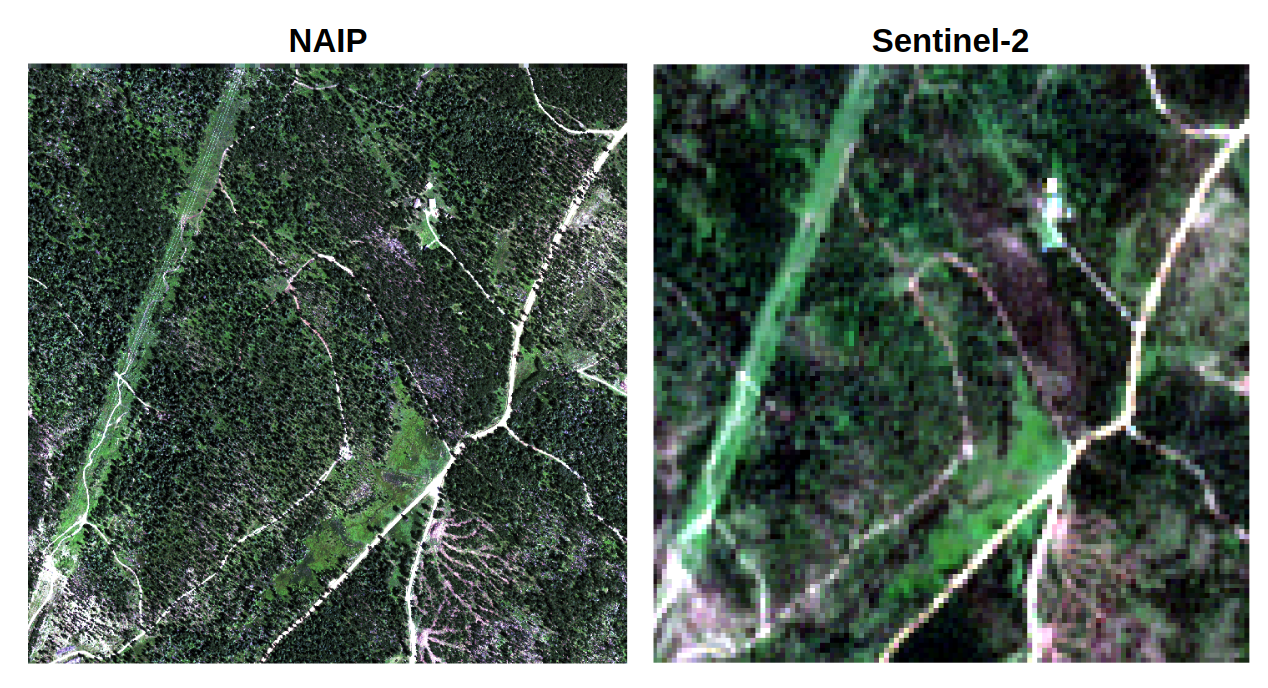
\includegraphics[width=1\linewidth]{images/csaybar_fig02.png}
    \begin{justify}
        \textit{Note.} Comparison between Sentinel-2 and NAIP near Rapid City, South Dakota. The Sentinel-2 image (rigth) has a spatial resolution of 10 meters, while the NAIP image (left) has a spatial resolution of 0.6 meters.
    \end{justify}                    
    \label{fig:naip_comparison}
\end{figure}


\subsection{OpenSR dataset}
The OpenSR dataset is an extensive dataset designed to facilitate the development of standard and reference single-image super-resolution algorithms for Sentinel-2 imagery. The high-resolution (HR) images in this dataset are sourced from the National Agriculture Imagery Program (NAIP), which provides aerial imagery covering the entire contiguous United States.

NAIP collects data across various spectral bands, including red, green, blue, and near-infrared, at a resolution of 0.6 m/pixel.

\subsection{WorldStrat Dataset}
The World Stratified Dataset, also known as WorldStrat, is a curated and diverse dataset. Its primary purpose is to aid in the development of multi-frame super-resolution algorithms specifically designed for Sentinel-2 imagery. A key feature of this dataset is the inclusion of high-resolution (HR) imagery from the SPOT 6/7 satellites. The SPOT imagery encompasses five distinct spectral bands. The panchromatic (PAN) band is at 1.5 m/pixel and the remaining bands, include Red, Green, Blue, and Near Infrared (RGBNIR) at 6 m/pixel.

The dataset covers approximately 10000 square kilometers and includes 3504 distinct areas of interest \ref{fig:worldstrat}, curated for the highest diversity of possible uses. The image acquisition budget for the dataset is divided into three parts:

\begin{itemize}
    \item \textbf{Settlement/Urban:} This part covers 3,647.5 square kilometers with 1,459 high-resolution images. The images are stratified sampling based on urban density (SMOD).
    \item \textbf{Non-Settlement}: This part covers 2,370 square kilometers with 948 high-resolution images. The images are stratified sampling based on land use (IPCC).
    \item \textbf{Underrepresented}: This part covers 3802.5 square kilometers with 1521 high-resolution images. The sources for these images include UNHCR, Amnesty, and ASMSpotter.
\end{itemize}

\begin{figure}[H] 
    \caption{\doublespacing \\ \textit{Summarizing the construction and classes of the WorldStrat dataset.}} 
    \centering
    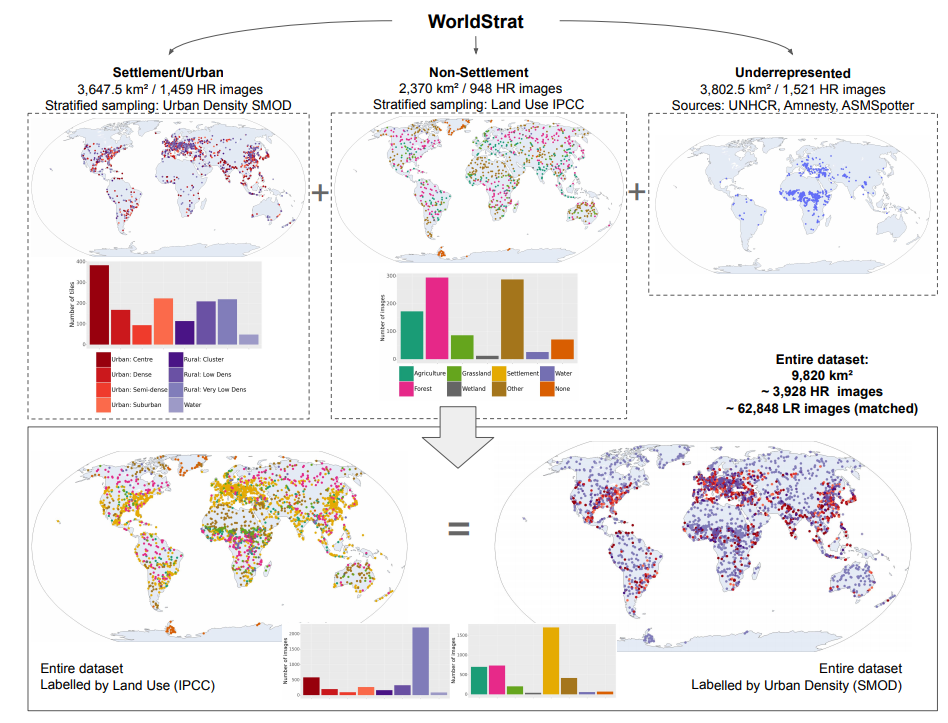
\includegraphics[width=1\linewidth]{images/csaybar_fig07.png}
    \begin{justify}
        \textit{Note.} Summarizing the construction and classes of the WorldStrat dataset. Obtained from \textcite{cornebise2022open}
    \end{justify}                    
    \label{fig:worldstrat}
\end{figure}


\subsection{Sen2Venus Dataset}

SEN2VENμS is a large dataset specifically designed to improve the spatial resolution of eight Sentinel-2 bands to 5 meters. It consists of cloud-free surface reflectance patches captured by Sentinel-2 L2A at 10 meters and 20 meters, along with corresponding reference patches acquired by the VENμS satellite at 5-meter resolution on the same day. The dataset covers 29 different locations worldwide, encompassing a total of 132,955 patches, each with a size of 256 × 256 pixels 

SEN2VENµS is a large dataset specifically designed to improve the spatial resolution of eight Sentinel-2 bands to 5 meters. It consists of cloud-free surface reflectance patches captured by Sentinel-2 L2A at 10 meters and 20 meters, along with corresponding reference patches acquired by the VENµS satellite at 5-meter resolution on the same day. The dataset covers 29 different locations worldwide, encompassing a total of 132,955 patches, each with a size of 256 × 256 pixels (Figure \ref{fig:sen2venus}).

\begin{figure}[H] 
    \caption{\doublespacing \\ \textit{Map of Sentinel-2 coverage on Theia (orange), available VENμS sites (green).}} 
    \centering
    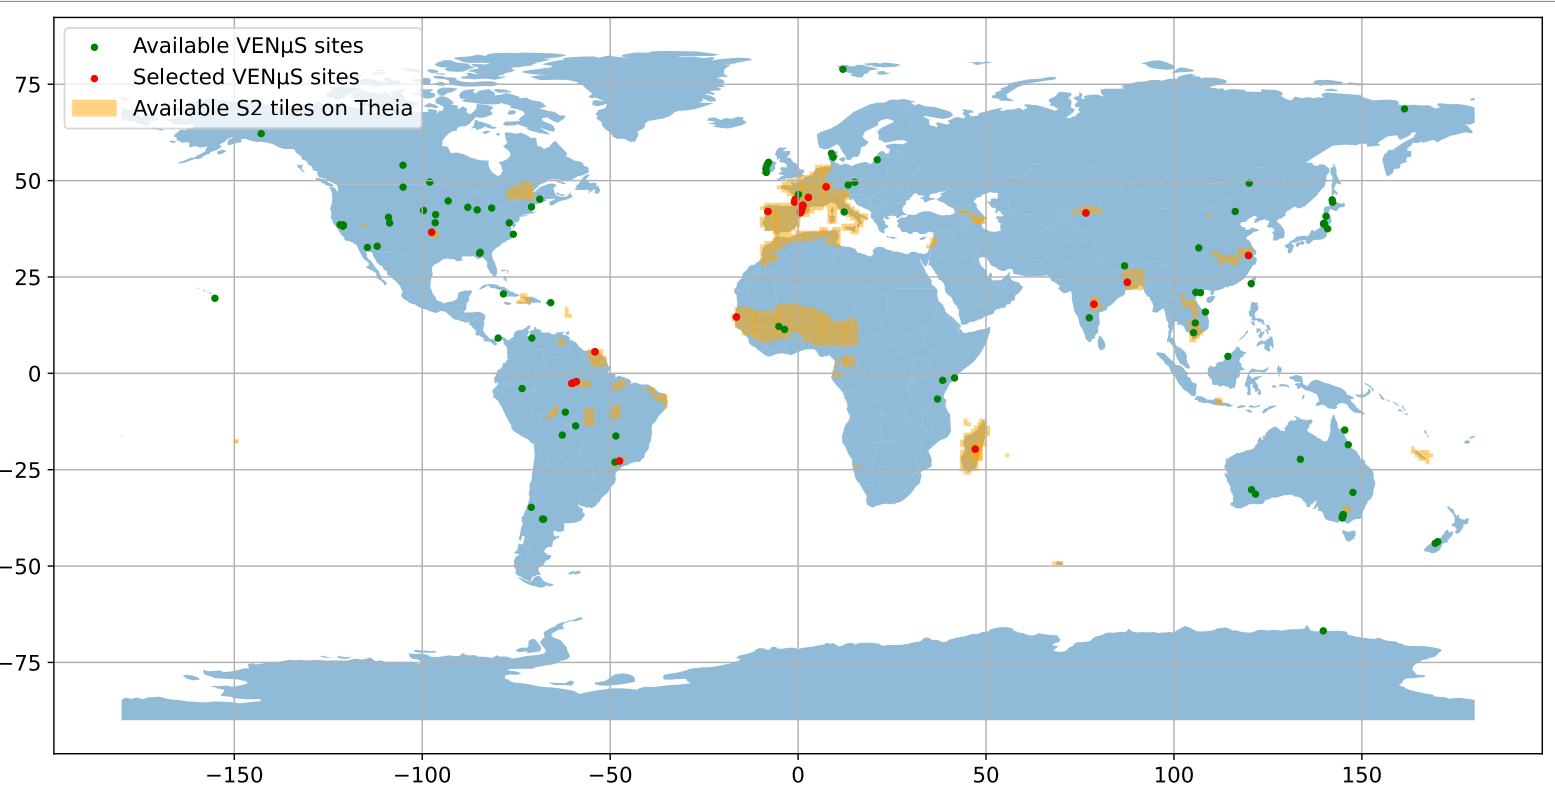
\includegraphics[width=1\linewidth]{images/csaybar_fig06.png}
    \begin{justify}
        \textit{Note.} Map of Sentinel-2 coverage on Theia (orange), available VENμS sites (green) and 29 selected sites (red) for the dataset. Obtained from \textcite{michel2022sen2venmus}
    \end{justify}                    
    \label{fig:sen2venus}
\end{figure}


\subsection{Degraded Sentinel-2 Dataset}

The datasets introduced above all have certain qualities and drawbacks. One of the factors to balance is dataset size compared to the quality and suitability of the data. On one end of the spectrum, WorldStrat is of very high quality and closely connected to the type of SR we want to perform, while on the other end the OpenImages dataset is huge while having no connection to remote sensing imagery. In order to have images in the spectral domain of Sentinel-2 and from the remote sensing domain, a large amount of Sentinel-2 RGB-NIR imagery has been sampled all over the world (Figure \ref{fig:sampling_sites}).

The images of course have the standard Sentinel-2 resolution of 10 meters, which is used as the $HR$ version. The $LR$ version of the image pair is created by applying a degradation kernel to the $HR$ image, producing a pair of $LR$-$HR$ RGB-NIR images that have 40 and 10m spatial resolution respectively, for a SR factor of 4. Over 250,000 image pairs are created this way, providing a dataset that has no problems with a spectral, temporal or geometrical mismatch and is already in the domain of Sentinel-2. The only drawback is that the frequency of information is changed since the scale of objects on the ground is vastly different. Still, this dataset is very useful in training the networks either from scratch or for a rougher finetuning after being trained on natural image datasets. After that, the NAIP and worldstrat datasets can provide the final touch.

\begin{figure}[H] 
    \caption{\doublespacing \\ \textit{Sampling areas (gray) and locations (red) of cloud-free Sentinel-2 images.}} 
    \centering
    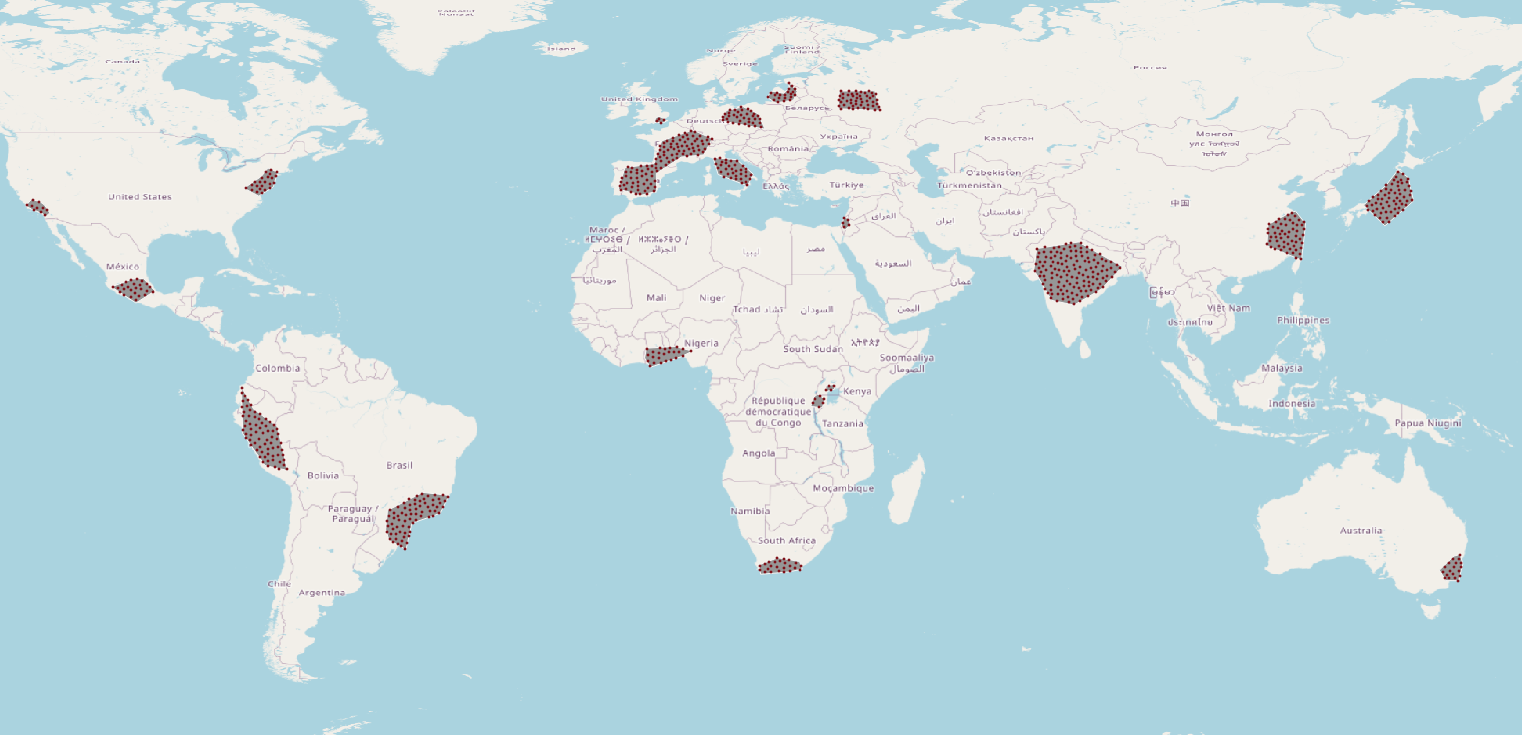
\includegraphics[width=1\linewidth]{images/sampling_locations.png}
    \begin{justify}
        \textit{Note.} Sampling areas (gray) and locations (red) of cloud-free Sentinel-2 images.
    \end{justify}                    
    \label{fig:sampling_sites}
\end{figure}

\begin{figure}[H] 
    \caption{\doublespacing \\ \textit{Example of the degraded Sentinel-2 dataset.}} 
    \centering
    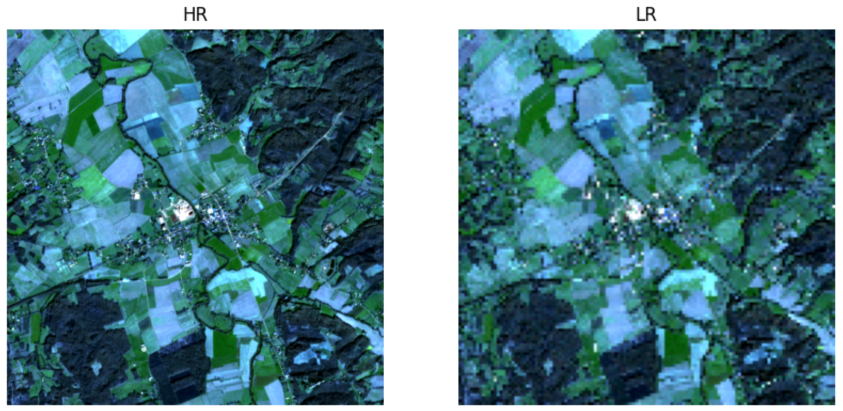
\includegraphics[width=1\linewidth]{images/sen2_degr.png}
    \begin{justify}
        \textit{Note.} Example of the degraded Sentinel-2 dataset (HR: 10m, LR: 40m). While the spectral properties as unmistakable Sentinel-2-like, the spatial information frequency is clearly different from 2.5m-10m datasets.
    \end{justify}                    
    \label{fig:sen2_degraded}
\end{figure}


\section{Data Harmonization}

\subsection{Effective spatial resolution and PSF}

Understanding the relationship between effective spatial resolution and the Point Spread Function (PSF) is essential for accurate interpretation of super-resolution models. In our study, the term effective spatial resolution is employed to denote the spatial resolution as gauged by the ground sampling distance, rather than simply characterizing it by the pixel size. The concept of ground sampling distance (GSD) refers to the system's capability to delineate small objects within an image. The GSD is influenced by various factors, including sensor design, viewing angle, and image pre-processing techniques. These factors can be effectively modeled using single or multiple PSFs (Figure \ref{fig:psf}).


\begin{figure}[H] 
    \caption{\doublespacing \\ \textit{A graphical depiction illustrating the Point Spread Function (PSF) of an optical imaging system.}} 
    \centering
    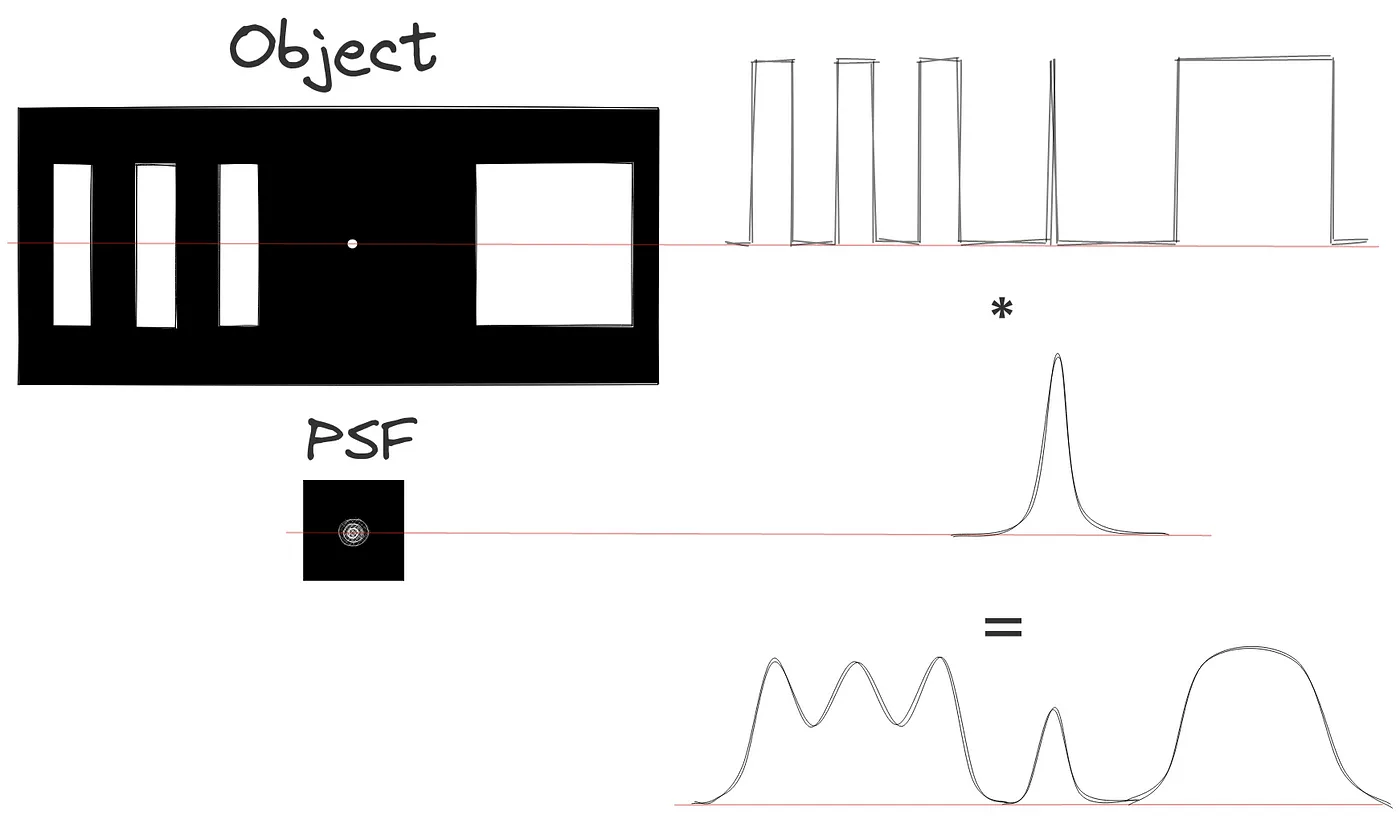
\includegraphics[width=1\linewidth]{images/csaybar_new_fig01.png}
    \begin{justify}
        \textit{Note.} A graphical depiction illustrating the Point Spread Function (PSF) of an optical imaging system. The extent of the spread directly impacts the spatial resolution, meaning that when it is larger, the ability to distinguish individual objects decreases.
    \end{justify}                    
    \label{fig:psf}
\end{figure}


The PSF characterizes the response of an imaging system to a point source or a single pixel. It describes how the energy from an object spreads out in the image, affecting image sharpness, resolution, and spatial accuracy. Through the modeling of the PSF attributes, it is possible to emulate the functionalities of low-resolution ($LR$) remote sensing systems using high-resolution ($HR$) counterparts.

\subsection{Spatial Co-registration}

In the realm of super-resolution, spatial co-registration serves as an essential preprocessing measure to mitigate disparities between high-resolution ($HR$) and low-resolution ($LR$) sensors. In practical scenarios, even marginal misalignments can considerably influence the precision of the resultant metrics. Consequently, guaranteeing meticulous spatial co-registration becomes indispensable for deriving trustworthy and insightful super-resolution metrics.

Spatial co-registration algorithms generally encompass three primary stages. The first stage is keypoint detection, which seeks to identify prominent points within an image. The next stage involves the detection of matching points between the $HR$ and $LR$ images. Lastly, the misalignment errors are calculated through a polynomial model fitted to these matching points. Over recent years, a plethora of algorithms for automated image alignment have been presented. For instance, the SEN2VENμS dataset utilized the SIFT matching algorithm \autocite{michel2022sen2venmus}, while MuRA-T compare the alignment outcomes of Fast+VGG and SuperPoint+SuperGlue algorithms \autocite{deshmukh2023aligned}.

\begin{figure}[H]
    \caption{\doublespacing \\ \textit{Matching points obtained by applying the SuperPoint + SuperGlue algorithm to a pair of images.}} 
    \centering
    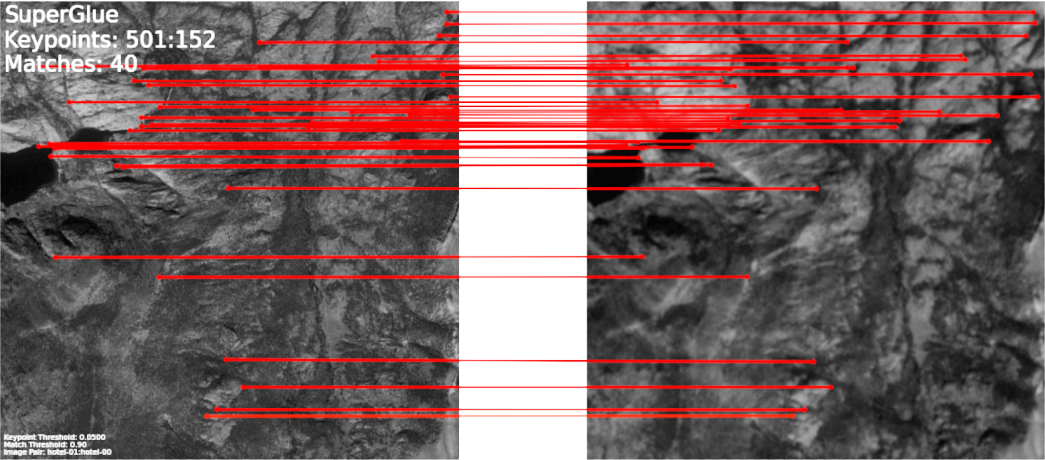
\includegraphics[width=1\linewidth]{images/csaybar_fig01.png}
    \begin{justify}
        \textit{Note.} Matching points obtained by applying the SuperPoint + SuperGlue algorithm to a pair of images, where the low-resolution (LR) image is from Sentinel-2 and the high-resolution (HR) image is from NAIP.
    \end{justify}                    
    \label{fig:coregistration}
\end{figure}

\subsection{Cross-instrument calibration and harmonization}
Even when two remote sensing sensors acquire data on the same day, significant variations in their values may still exist. These variations can be attributed to several factors, which include:


\begin{itemize}
    \item \textbf{Sensor characteristics}: Each sensor has its own unique spectral response function, which can result in variations in the reflectance values, even when the atmospheric conditions and viewing angle are the same.

    \item \textbf{Atmospheric conditions}: The atmosphere can undergo significant changes within a few minutes or seconds. These variations can impact the quality and accuracy of the data captured by remote sensing sensors. Atmospheric scattering, for example, can introduce variations in the sensor signals, leading to differences in reflectance values.

    \item \textbf{Viewing geometry}: The difference between the angle at which the sensors observe the Earth's surface, can also lead to variations in the reflectance values.

    \item \textbf{Calibration and preprocessing}: Each sensor goes through its own calibration process to convert the raw sensor measurements into meaningful reflectance values. These variations need to be carefully accounted for and addressed during $LR$-$HR$ comparison.
    
\end{itemize}

To minimize potential variations in reflectance between $LR$-$HR$ pairs, an additional component is proposed to enhance the classical degradation model.

\begin{equation}
    I_{LR} = \gamma[\delta(I_{HR}, \eta)] + \epsilon
\end{equation}

Where $I_{LR}$ is the $LR$ image, $I_{HR}$ is the $HR$ image, $\eta$ is a parameter from the degradation model $\delta$, $\epsilon$ represent the noise, and the $\gamma$ the harmonization model.
	\chapter{State of the Art}

\section{SR Design \& Implementation}
Diffusion \autocite{NEURIPS2020_4c5bcfec} models have recently overtaken GAN \autocite{NIPS2014_5ca3e9b1} models in the state-of-the-art of generative image methodologies \autocite{10081412}. While GANs have been extensively used in image super-resolution \autocite{9044873}, they are unstable due to their very delicate training process. Diffusion models, which are also probabilistic models drawing results from a likelihood distribution, have proven to be easier to train and deliver better results, surpassing other methodologies in many reconstruction metrics \autocite{saharia2021image}. This development has also been noticed in the remote sensing community, with recent super-resolution papers switching to diffusion-based SR methodologies \autocite{rs14194834, 10057005, 103389fmars20231211981}.

\begin{figure}[H]
    \caption{\doublespacing \\ \textit{Pixel-space (above) and latent-space (below) diffusion models.}} 
    \centering
    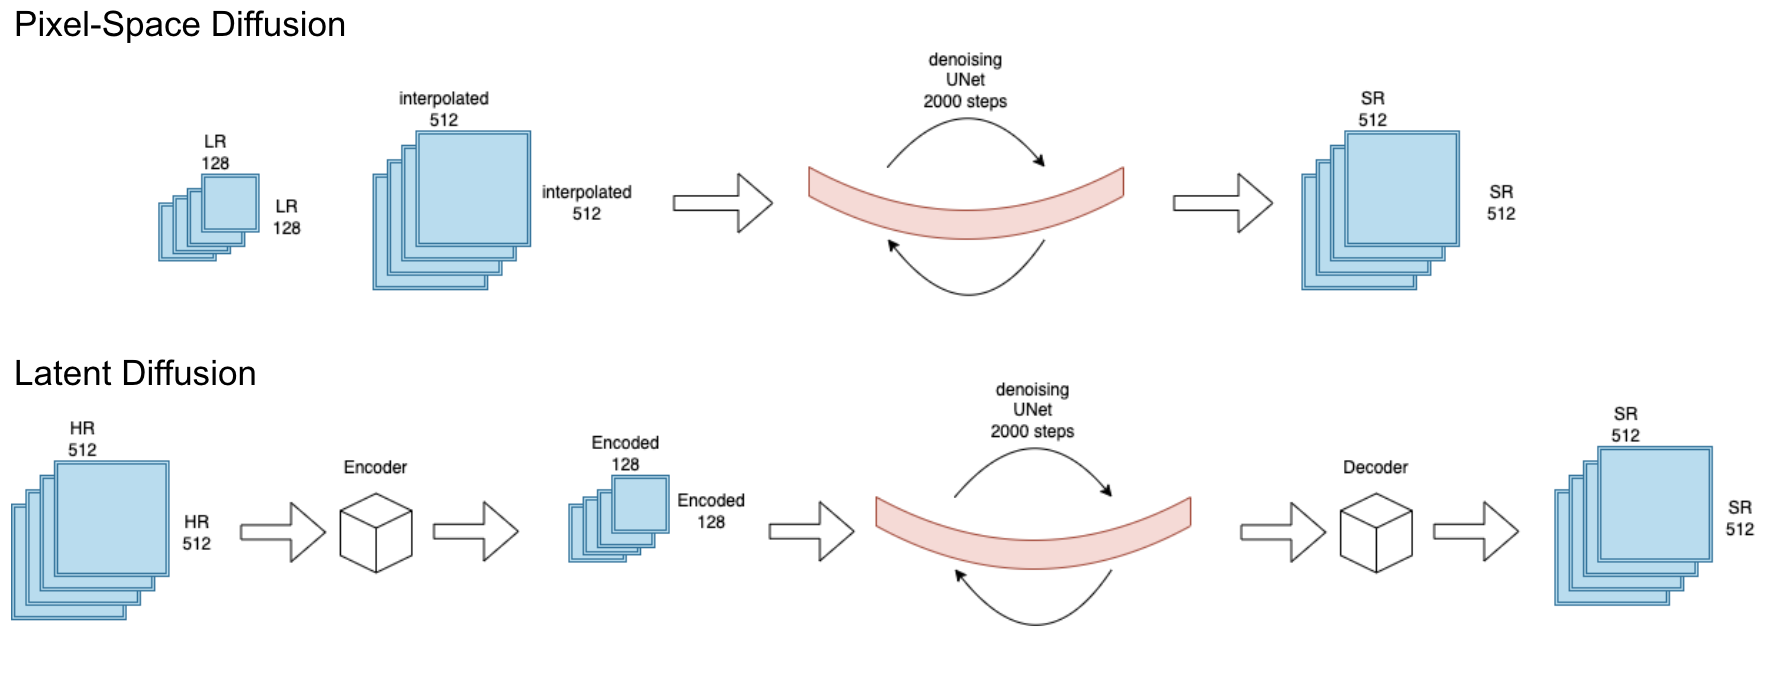
\includegraphics[width=1\linewidth]{images/lat_px_dif.png}
    \begin{justify}
        \textit{Note.} Pixel-space (above) and latent-space (below) diffusion models.
    \end{justify}                    
    \label{fig:pixel_latent_space}
\end{figure}

\subsection{Latent-Diffusion vs Pixel-Space Diffusion}

Most SR models found in the literature use pixel-space diffusion (see Figure \ref{fig:pixel_latent_space}, top). In this workflow, the $LR$ image is interpolated to the desired size. The denoising U-Net, which is cycled through \textit{n} times, removing a small amount of noise in each iteration. This method is very computationally expensive, since each image that needs to be super-resoluted has to pass many times through the whole network to receive the output. In general, 500 to 2000 of these iterations are used.

Latent diffusion models on the other hand perform the computationally expensive denoising steps on a lower-dimension representation of the input image (see fig. \ref{fig:pixel_latent_space}, bottom). A separate network, the autoencoder, generates a latent space and smaller than the original input space and therefore makes the denoising step much faster. After the denoising, the image is decoded and inflated again to the original desired dimensionality of the SR product. It has been shown that performing latent diffusion significantly reduces computational requirements while preserving the powerful SR capabilities of diffusion models \autocite{rombach2022highresolution}.


\subsection{Codebase}

Several code-bases related to super-resolution (SR) models have been developed and are available for exploration and implementation (see fig. \ref{fig:codebase}). Among them, two unofficial implementations of the SR3 model \autocite{saharia2021image} stand out: one hosted on \href{https://github.com/Janspiry/Image-Super-Resolution-via-Iterative-Refinement}{GitHub by Janspiry} and another by \href{https://github.com/KiUngSong/Generative-Models/tree/main/SR3}{KiUngSong}. While these repositories provide valuable insights into SR3’s functionality, they focus on pixel-space diffusion and have received feedback from the community regarding certain design choices and limitations in code quality and expandability. Additionally, these implementations tend to yield medium-quality results.


\begin{figure}[H]
    \caption{\doublespacing \\ \textit{Codebases in use.}} 
    \centering
    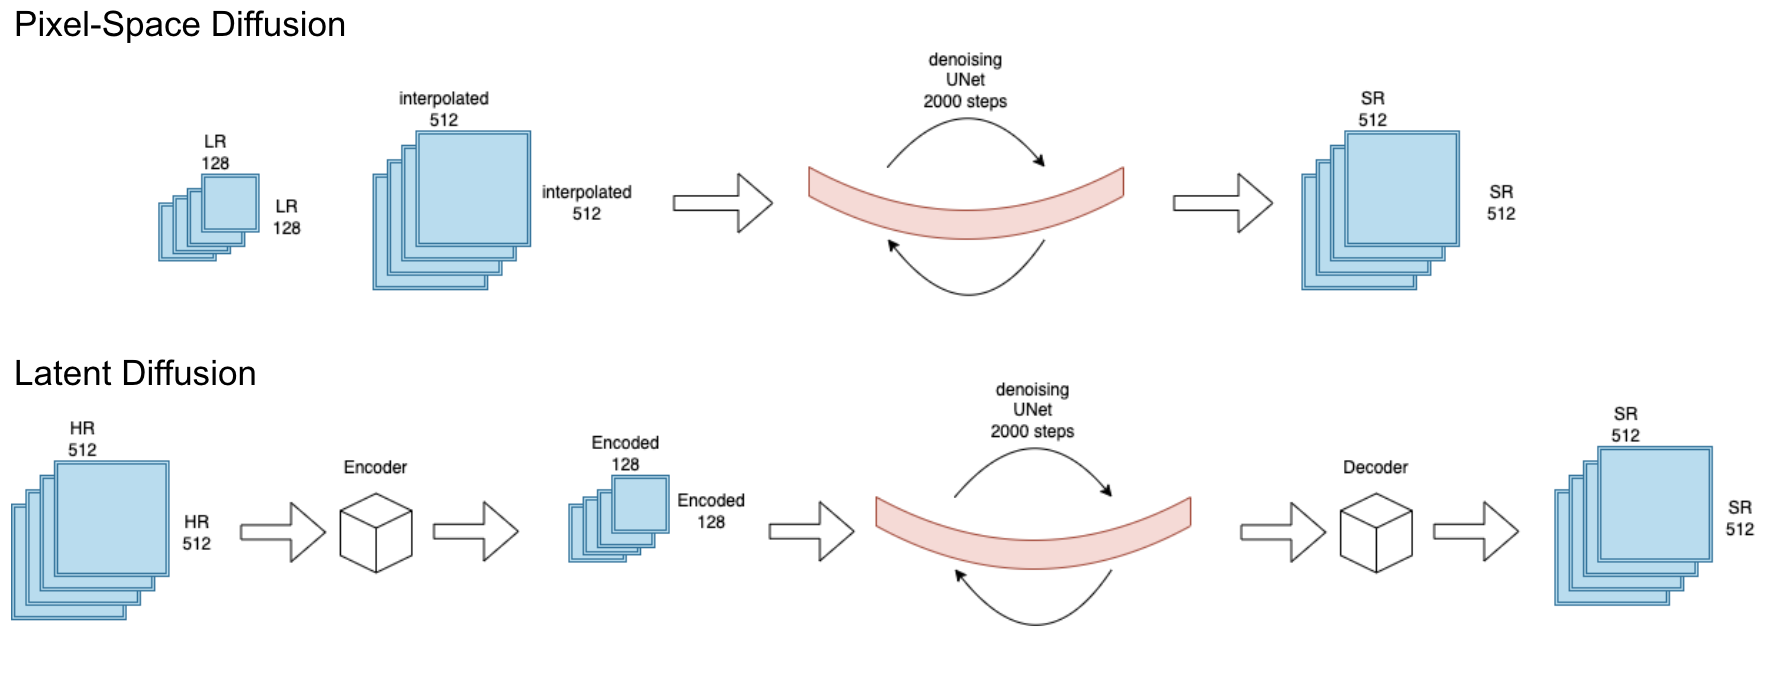
\includegraphics[width=1\linewidth]{images/lat_px_dif.png}
    \begin{justify}
        \textit{Note.} Codebases in use.
    \end{justify}                    
    \label{fig:codebase}
\end{figure}

Another noteworthy resource is the \href{https://github.com/mikonvergence/DiffusionFastForward}{DiffusionFastForward} repository, which serves as a clear tutorial-like implementation for both pixel-space and latent-space diffusion models. However, it is relatively simple and heavily reliant on external repositories, limiting its scalability and modifiability. Despite its simplicity, it offers a good understanding of the core diffusion strategies for SR.

Finally, the \href{https://github.com/mikonvergence/DiffusionFastForward}{latent-diffusion} repository, the official code-base of the highly successful latent-diffusion model \autocite{rombach2022highresolution}, offers a comprehensive solution that encompasses various tasks such as unconditional image generation, text-prompt-based image generation, inpainting, and super-resolution. This repository is known for its versatility and well-organized structure, making it highly adaptable for further modifications and expansions. The availability of pre-trained checkpoints provided by the authors also allows for immediate demonstration of the model’s strong capabilities, positioning it as a leading resource for super-resolution projects.


\subsection{Autoencoder}

The autoencoder under consideration is designed to compress the spatial dimension by a factor of 4, reducing tensors from \textit{4$\times$512$\times$512} to \textit{4$\times$128$\times$128} before decoding them back to their original dimensions. This approach is inspired by the \textit{latent-diffusion} repository, as described in \autocite{rombach2022highresolution}. Ideally, such encoding and decoding processes aim to preserve image quality. Beyond reconstruction metrics, the latent space produced by the autoencoder plays a crucial role in super-resolution, as the denoising occurs after the encoder. This type of autoencoder has been effectively utilized in various applications, as demonstrated by the latent diffusion model and its adaptations in prior research \autocite{esser2021taming}.

In this context, models are often trained independently from the denoising U-Net, using a combination of perceptual LPIPS and a GAN component. The GAN component typically employs a classifier that distinguishes between real images and reconstructed images, where the output logits are combined with the perceptual loss and then back-propagated through the autoencoder. The LPIPS metric \autocite{zhang2018unreasonable} is widely used in computer vision tasks, simulating human visual perception to return a similarity score between two images. Since LPIPS is based on a VGG network \autocite{simonyan2015deep} and is primarily trained on RGB data, extending it to handle more than 3 bands presents challenges, especially for 4-band models like RGB-NIR. In such cases, a common workaround involves selecting 3 bands at random during each training step and feeding them into the LPIPS model. Although unconventional, this method has been validated, as random permutations of the 4-band tensor into 3 bands have shown no significant loss in LPIPS accuracy. Figure \ref{fig:lpips_permutation} demonstrates that the LPIPS boxplot results for 200 interpolated LR-HR image pairs remain consistent, even when using spectral band combinations that were not part of the original training, thus supporting the viability of this approach.


\begin{figure}[H]
    \caption{\doublespacing \\ \textit{LPIPS boxplots for all possible 3 band permutations from the 4 band tensors.}} 
    \centering
    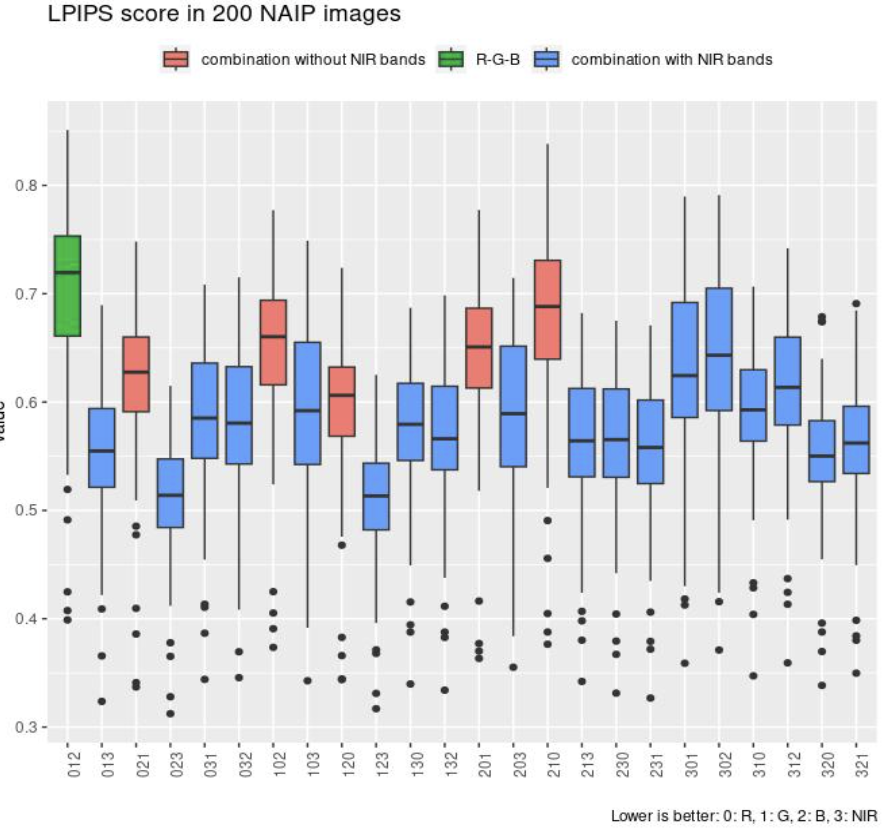
\includegraphics[width=1\linewidth]{images/lpips_permutation.png}
    \begin{justify}
        \textit{Note.} LPIPS boxplots for all possible 3 band permutations from the 4 band tensors.
    \end{justify}                    
    \label{fig:lpips_permutation}
\end{figure}


\begin{figure}[H]
    \caption{\doublespacing \\ \textit{Minimum (light red), mean (orange), standard deviation (green), and maximum (blue) of the encoded value ranges.}} 
    \centering
    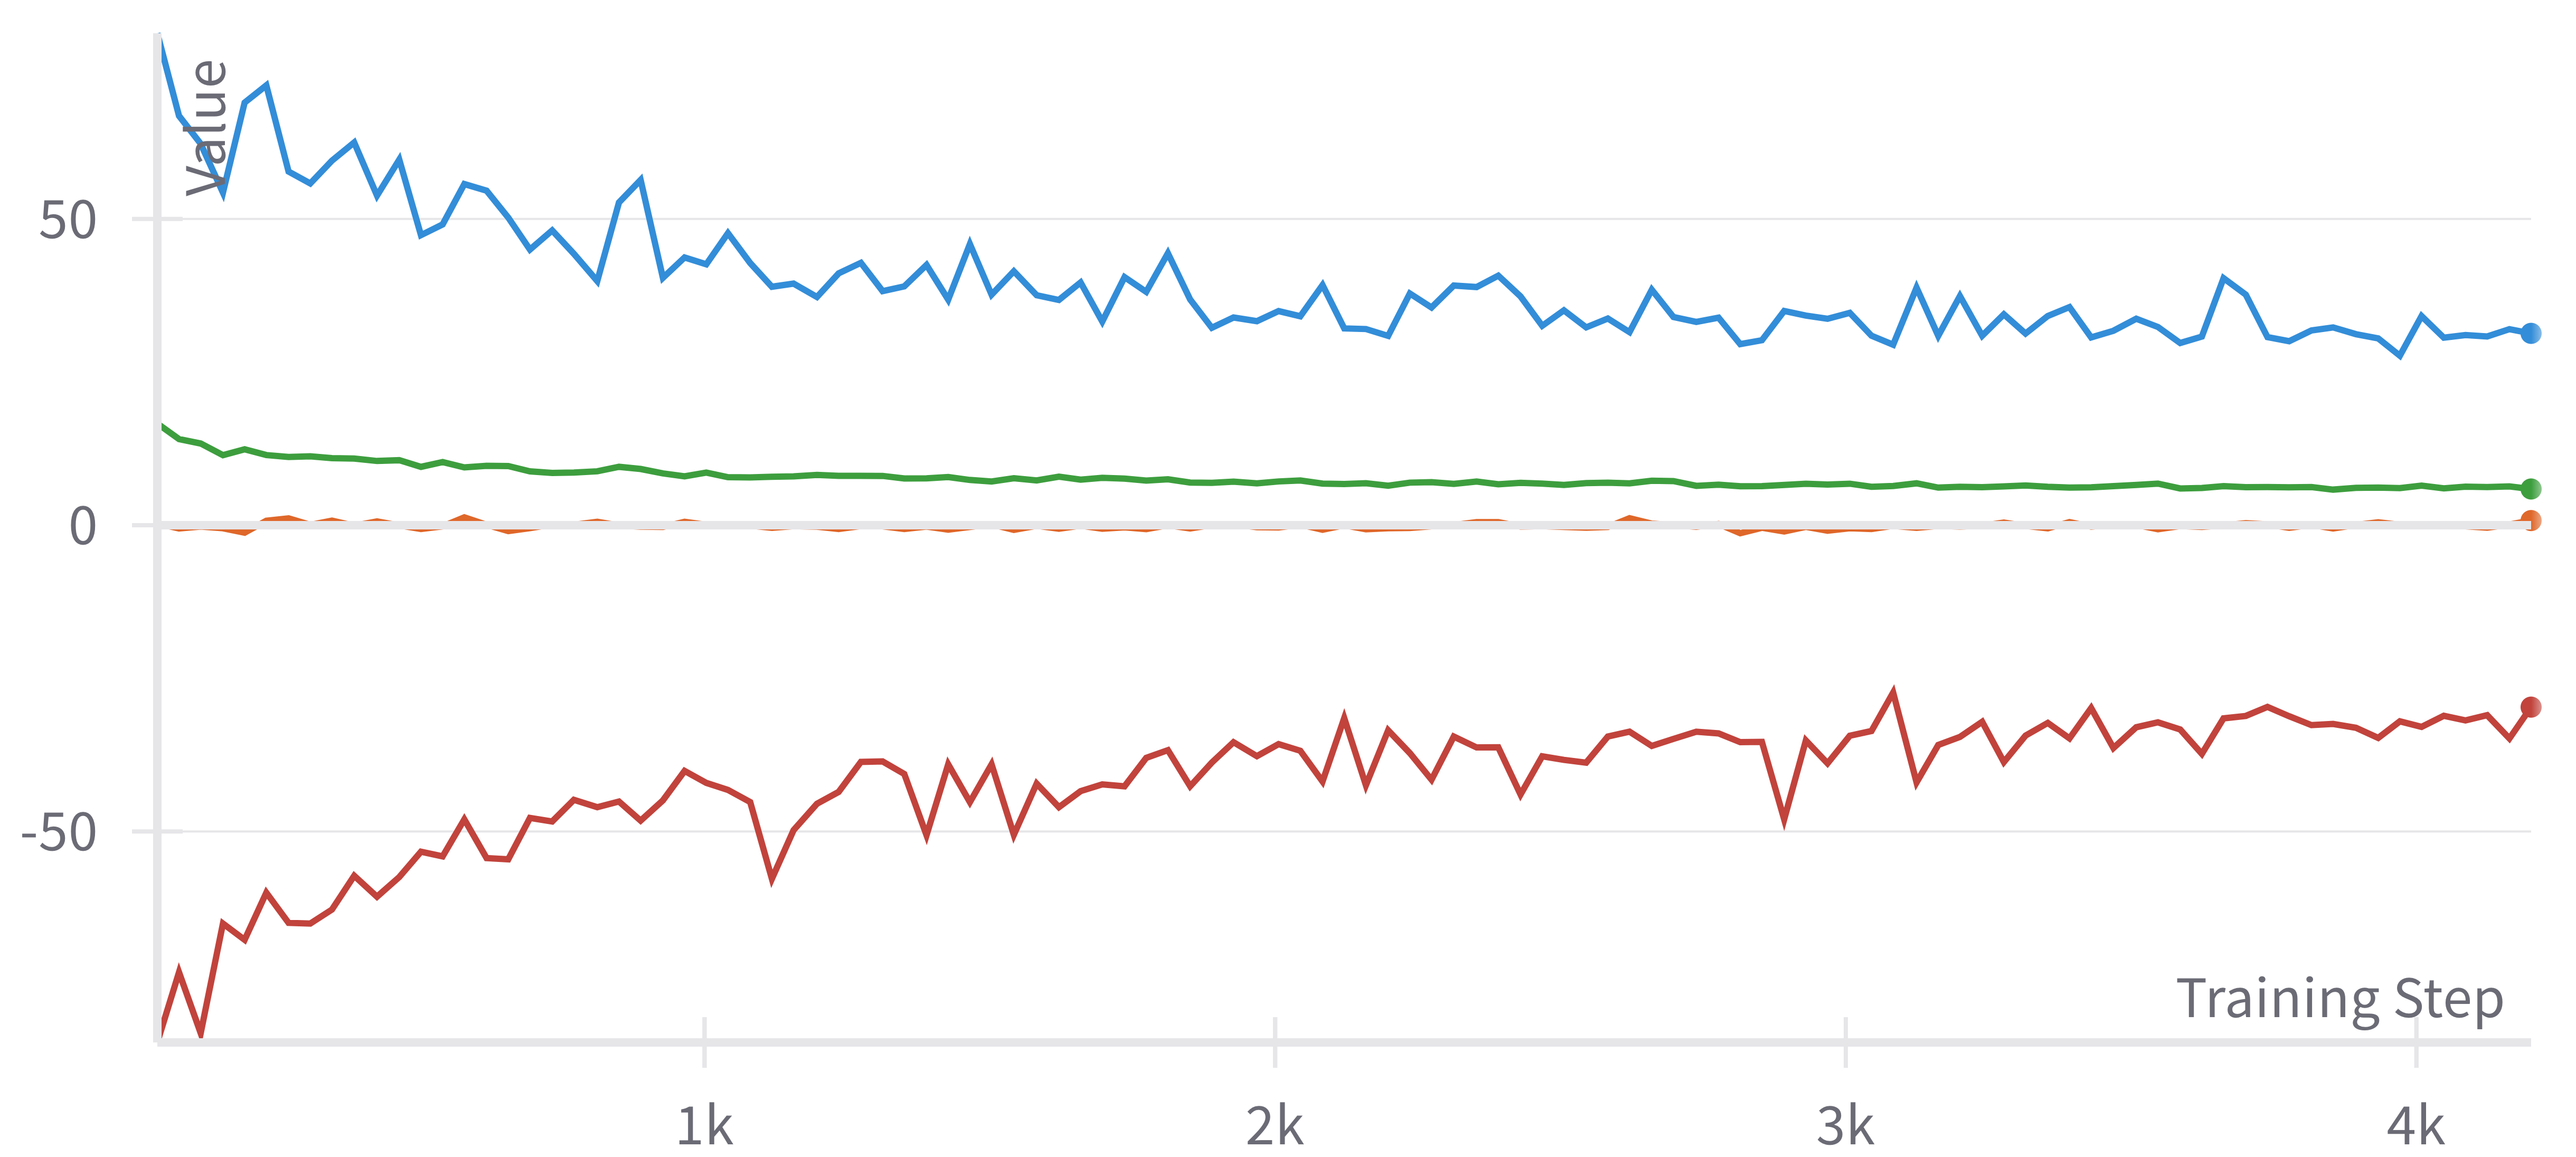
\includegraphics[width=1\linewidth]{images/simon/ae_distr_enc.png}
    \begin{justify}
        \textit{Note.} Minimum (light red), mean (orange), standard deviation (green), and maximum (blue) of the encoded value ranges during AE training. While we want the value range to be similar to the input images, if the value range is compressed too much we lose the ability to recover the images accurately.
    \end{justify}                    
    \label{fig:ae_distr_enc}
\end{figure}


Additionally, an autoencoder with Kullback-Leibler regularization is used to ensure that the latent space closely mirrors the input image distribution. This regularization penalizes the encoder when the encoded image strays too far from the original image distribution, which is particularly crucial during the inference stage, where the encoding process is skipped, and the image is directly denoised and super-resolved from \textit{128$\times$128} $LR$ dimensions to \textit{512$\times$512} $HR$ dimensions in the decoder. Maintaining the encoded image distribution as close as possible to the $LR$ image (minus the noise) is key to achieving high-quality results.

Balancing the regularization of the encoded values is essential to ensuring that the encoded image remains similar to the input, while also capturing enough variation. Over-regularization, such as reducing the extremes or standard deviation of the latent space too much, can degrade reconstruction quality (see \autoref{fig:ae_distr_enc}). Empirical evidence suggests that a standard deviation around 5 strikes the optimal balance. By leveraging 32-bit floating-point numbers, this process effectively translates some of the high-resolution spatial complexity into numerical representation. Without this complexity, the reconstruction quality suffers.

Training the autoencoder (AE) is a delicate process. While the decoder's output converges rapidly—visually reconstructing the input image quite quickly—the resulting model checkpoint is not immediately ready for integration into the super-resolution (SR) workflow. The GAN component requires a warm-up period before its loss is weighted, and the regularization needs time to take effect. Furthermore, the autoencoder requires a large amount of satellite imagery data for training due to its size, with over 72 million parameters.

\begin{figure}[H]
    \caption{\doublespacing \\ \textit{Visualization of the original image, the encoded image, and the recovered image (f.l.t.r.).}} 
    \centering
    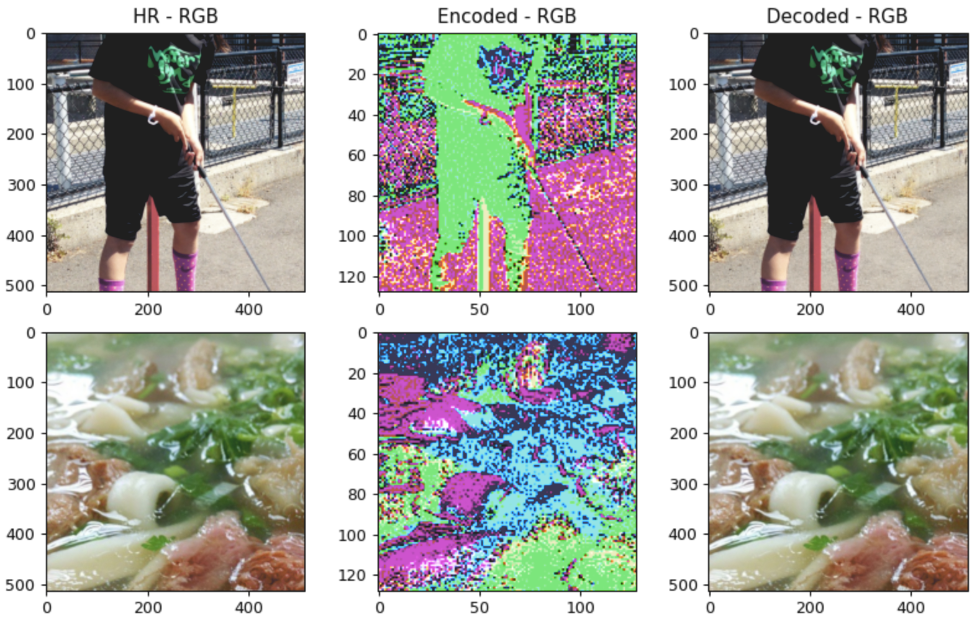
\includegraphics[width=1\linewidth]{images/autoencoder.png}
    \begin{justify}
        \textit{Note.} Visualization of the original image, the encoded image, and the recovered image (f.l.t.r.).
    \end{justify}                    
    \label{fig:autoencoder}
\end{figure}


\autoref{fig:autoencoder} illustrates that while the image is faithfully reconstructed, the latent space might not yet be optimized for SR with the U-Net. Extensive training, careful learning rate schedules, and warm-up periods, along with latent space regularization, are required to avoid this issue.

\subsection{Denoising UNet}
The denoising probabilistic model is designed to iteratively predict a denoised version of the input image by learning the input data distribution. This process can be described as a Markov chain, where each timestep determines both preceding and following states. By learning the distribution $p(x)$ of the input data, the model is able to reverse the chain and produce denoised images. The training minimizes the variational lower bound on the log-likelihood of the data under the model, penalizing outputs that fall on the lower end of the probability scale with respect to the target distribution.

The denoising model uses a U-Net backbone, augmented with noise-adding functions that handle both the addition and removal of normally distributed noise. Since the autoencoder handles a 4x upscaling, the model can be conditioned on the $LR$ image. Therefore, instead of starting from a pure noise image, the denoising process begins with the $LR$ image and progressively removes noise, recovering lost quality before the image is upscaled by the autoencoder. This approach has been successfully demonstrated by \autocite{rombach2022highresolution} for various tasks, such as conditional and unconditional image generation, inpainting, style transfer, and super-resolution. In this workflow, the U-Net is conditioned on the $LR$ image in the original spectral domain, specifically in the RGB-NIR color space (see \autoref{fig:encLR_schema}).

\subsubsection{UNet Adaptations}
As the autoencoder's sampling process expects a distribution similar to that of its own training (see \autoref{fig:ae_distr_enc}), the U-Net implicitly learns to transform the input spectral distribution into the encoded spectral distribution. Although this transformation does not affect spatial feature reconstruction, it does impact the spectral consistency of the SR image. To mitigate this, we interpolate the $LR$ image to the same dimensions as the $HR$ image before encoding. This change relieves the U-Net from the burden of learning the mapping between the two spectral domains (\autoref{fig:encLR_schema}). During training, this results in a conditioning that concatenates the noise-encoded $HR$ tensor with the same-size $LR$ image, rather than mixing spectral domains. At inference, the encoded $HR$ image is replaced by only the noise tensor from the scheduler.

Experimentation demonstrates that the interpolated $LR$ image can be easily encoded and decoded by the autoencoder, even though the AE was trained on $HR$ images (\autoref{fig:encLRint_demo}). Although this adds an additional pass through the AE, it does not significantly increase processing time during training or inference.

\begin{figure}[H]
    \caption{\doublespacing \\ \textit{Schema of the changes to the UNet SR workflow.}} 
    \centering
    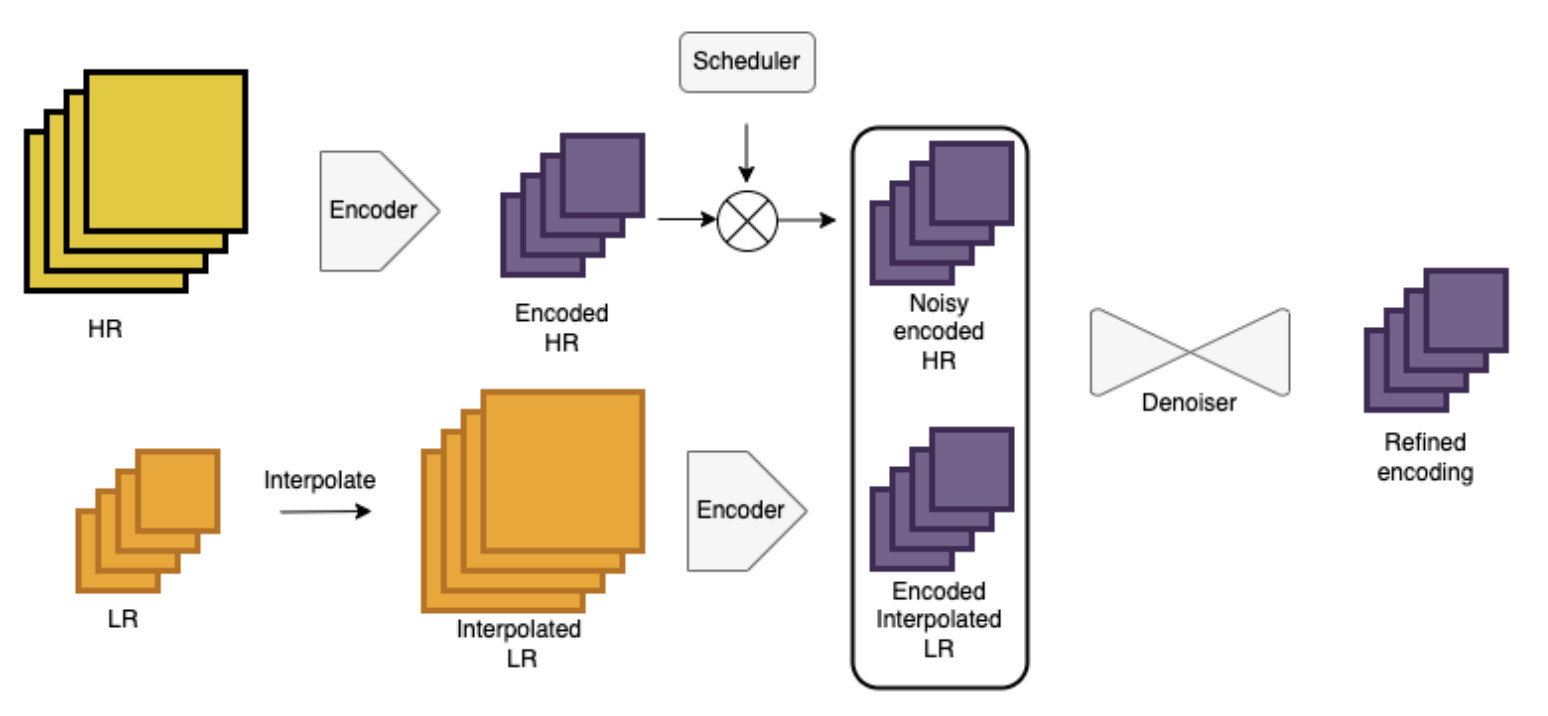
\includegraphics[width=1\linewidth]{images/simon/encLR_schema.png}
    \begin{justify}
        \textit{Note.} Schema of the changes to the UNet SR workflow. The denoising is conditioned on an interpolated and encoded $LR$ image rather than the original $LR$ image.
    \end{justify}                    
    \label{fig:encLR_schema}
\end{figure}

\begin{figure}[H]
    \caption{\doublespacing \\ \textit{Visualization of an interpolated (left), encoded (middle), and decoded (right).}} 
    \centering
    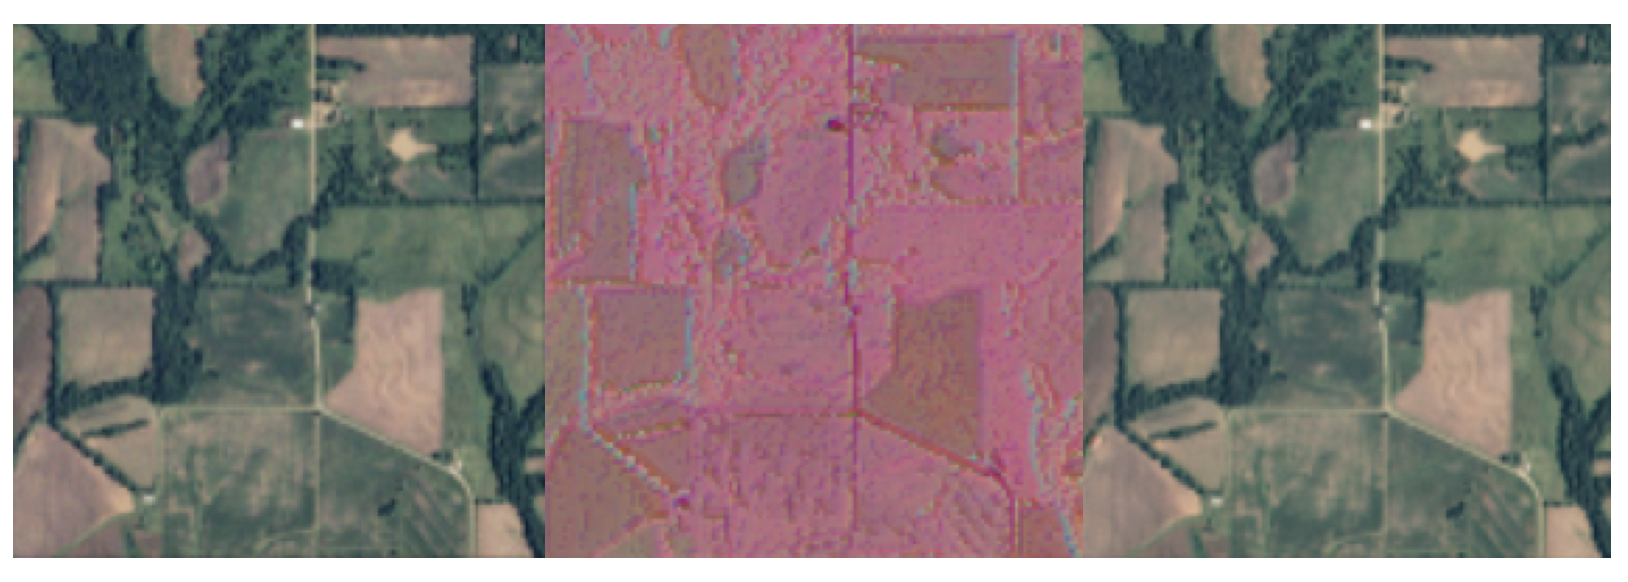
\includegraphics[width=1\linewidth]{images/simon/encLRint_demo.png}
    \begin{justify}
        \textit{Note.} Visualization of an interpolated (left), encoded (middle), and decoded (right) version of the same image. This demonstrates that the AE, even though trained on $HR$ imagery, can accurately process interpolated $LR$ images.
    \end{justify}                    
    \label{fig:encLRint_demo}
\end{figure}



\subsection{Multispectral 20m Band SISR Methodology}
The previous methodologies describe the performance of 4-band RGB-NIR SR on the S2NAIP dataset. To perform SR on the 20m bands of Sentinel-2, certain adaptations are necessary. %First, the synthetic dataset detailed in \autoref{sec:S2NAIP} is utilized.% 

While this dataset does not exactly match the spectral characteristics of the 20m Sentinel-2 bands, it is already adapted between $LR$ and $HR$, spatially co-registered, and degraded using degradation kernels optimized for this task. Since training is performed with random permutations and random ordering of the bands, the models ideally learn the degradation kernels and the spatial frequencies present in the 20m bands, while remaining agnostic to specific bands or values.

A 6-band autoencoder is trained on the described dataset, followed by the training of a 6-band U-Net to perform the actual SR task. These changes necessitate training from scratch.  %The same model descriptions in \autoref{autoencoder}, \autoref{unet}, and \autoref{unet_adaptations} are applicable to the 6-band version. 
While the same spatial features and frequencies apply to both the 10m and 20m bands, they are not interchangeable and must not be used in the same model. The easiest and most efficient approach is to train separate models for each band type, as shown in \autoref{table:sentinel2_bands_model}.


\begin{table}[H]
    \caption{\doublespacing \\ \textit{Model types for the different Sentinel-2 MSI bands.}}
    \begin{spacing}{8}
        \fontsize{8pt}{2pt}\selectfont  
        \begin{tabularx}{\linewidth}{P{6cm}*{4}{c}} 
            \toprule
            \textbf{Band Number} & \textbf{Band Description} & \textbf{Resolution (m)} & \textbf{Model Type} \\
            \midrule
            B1 & Coastal aerosol & 60 & - \\
            B2 & Blue & 10 & 4-band \\
            B3 & Green & 10 & 4-band \\
            B4 & Red & 10 & 4-band \\
            B5 & Vegetation Red Edge & 20 & 6-band \\
            B6 & Vegetation Red Edge & 20 & 6-band \\
            B7 & Vegetation Red Edge & 20 & 6-band \\
            B8 & NIR & 10 & 4-band \\
            B8A & Narrow NIR & 20 & 6-band \\
            B9 & Water Vapor & 60 & - \\
            B10 & SWIR - Cirrus & 60 & - \\
            B11 & SWIR & 20 & 6-band \\
            B12 & SWIR & 20 & 6-band \\
            \bottomrule
        \end{tabularx}
    \end{spacing}
    \vspace{1\baselineskip}
    \textit{Nota.} Model types for the different Sentinel-2 MSI bands.
    \label{table:sentinel2_bands_model}
\end{table}


\section{SISR Training Strategy}
The datasets used in this study and their properties are detailed in \autoref{chapter:datasets}. This section outlines how these datasets are leveraged during the training process for SR models. Due to the high parameter count of the autoencoder and denoising U-Net, large quantities of training data are required. The original authors \autocite{rombach2022highresolution} trained their models using the OpenImages dataset, which contains millions of images. For RGB super-resolution tasks, it is possible to fine-tune the well-optimized checkpoints from these authors using remote sensing imagery. Despite the limited availability of training images in this domain, fine-tuning can be sufficient for this task.

\paragraph{RGB-NIR SISR}
For RGB-NIR SR, training from scratch is required, as no pre-trained models are available for 4-band input. Therefore, large datasets are needed. The following training strategy utilizes different datasets in a sequential manner to take full advantage of their strengths:

\begin{enumerate}
    \item \textit{CV natural images dataset}: This dataset, compiled for this project, contains approximately 280k images. Although it only includes RGB images, we generate the missing fourth band by appending the intensity level of the image as the 4th band. This method is not identical to the NIR band but provides useful spatial and spectral information, as the intensity level is normalized to the same range as the other datasets.
    \item \textit{Sentinel-2 degraded dataset}: Following initial training with natural images, remote sensing data is used. This dataset includes 240k images, although it lacks the spatial properties specific to the research question, as the $LR$ version has a resolution of 40m and the $HR$ version has 10m resolution. However, as it consists of remote sensing images with the same spectral properties as Sentinel-2 data, it helps train the model on relevant spectral and spatial features.
    \item \textit{NAIP dataset}: This dataset closely resembles both the spatial and spectral properties of Sentinel-2 data. The $LR$ version is at 2.5 meters, matching the Sentinel-2 sensor's spectral characteristics, while the $HR$ version is at 2.5m. With 250k images, this dataset alone is sufficient for training from scratch. However, pretraining on previous datasets makes the models more robust.
    \item \textit{Worldstrat dataset}: With only 3k images, this dataset is too small for standalone training or fine-tuning, as the model will overfit. Furthermore, it uses a cross-sensor approach, complicating verification of synthetic results. The final SISR models are not trained on this dataset.
\end{enumerate}

\paragraph{20m-band Multispectral SISR}
The 6-band model follows a similar training strategy. By generating synthetic 6-band S2NAIP datasets, the training process remains consistent through repetition and permutation strategies. The training proceeds as follows:

\begin{enumerate}
    \item \textit{CV natural images dataset}: This dataset serves as the initial training phase, leveraging its abundant data.
    \item \textit{Sentinel-2 degraded dataset}: After pretraining, the model is refined on Sentinel-2 data to focus on satellite-specific image features. However, the interpolation and SR from 80m to 20m introduce challenges with different degradation kernels.
    \item \textit{NAIP dataset}: The 250k images in this dataset serve as the best approximation for the degradation problem at hand, with spatial and spectral similarities making it ideal for training the SR models.
\end{enumerate}

These training strategies enable the 4-band and 6-band models to evolve gradually, moving from a general approach to image reconstruction and SR towards the specific spatial and spectral requirements of the research question.

\subsection{Cross-sensor vs synthetic data}
Various deep learning techniques for super-resolution in earth observation have been proposed \autocite{wang2022review, liu2021research, sdraka2022deep}. These methods are broadly classified into cross-sensor and synthetic approaches. Cross-sensor algorithms require careful spatial alignment and spectral matching of $HR$ and $LR$ pairs, often constrained by the need for large-scale datasets. Synthetic methods, on the other hand, generate $LR$ images by degrading $HR$ images through a blur kernel and downsampling, though domain gaps between synthetic and real-world data remain a challenge \autocite{dong2022real, qiu2023cross, zhang2022single}.

	\chapter{Objetives}
\section{General objective}

The general aim of this project is to develop a super-resolution model capable of improving the spatial resolution of Sentinel-2 images from 10 meters and 20 meters to 2.5 meters using a combination of convolutional neural networks and multispectral data fusion techniques. The goal is to enhance both the spatial detail and spectral consistency of the images to support advanced geospatial analysis.

\section{Specific objectives}

\begin{enumerate}
    \item \textbf{To explore and implement advanced image fusion techniques:} The aim is to combine multispectral bands from Sentinel-2 and other sources (such as NAIP) to enhance spatial and spectral resolution.
    \item \textbf{To design and develop a deep learning-based super-resolution model:} The focus will be on creating a neural network model capable of processing the multispectral data to produce high-resolution outputs while preserving spectral integrity.
    \item \textbf{To apply the Wald Protocol for validation:} This involves using the Wald Protocol to ensure that the super-resolved images maintain consistency with the original images in terms of spatial and spectral properties.
    \item \textbf{To evaluate the performance of the proposed model:} The objective is to assess the model's performance through qualitative and quantitative metrics, comparing it with existing super-resolution techniques.
\end{enumerate}
	
	% \chapter{INTRODUCCIÓN}
\markboth{CAPÍTULO \thechapter: INTRODUCCIÓN}{}
	\section{GENERALIDADES}

\lipsum[5]
	\input{2_CAPITULO1/Secciones/2_Descripción del problema.tex}
	\section{OBJETIVOS DEL ESTUDIO}
	\subsection{Objetivo General}

	\lipsum[2]
	
	\subsection{Objetivos Específicos}
\begin{itemize}
\item Objetivo específico 1.

\item Objetivo específico 2.

\item Objetivo específico 3.

\end{itemize}





	
	\input{2_CAPITULO1/Secciones/4_Hipótesis.tex}
	\input{2_CAPITULO1/Secciones/5_Metodología.tex}
	


 % INTRODUCTION
	% PLAN DE TESIS
	% \chapter{INTRODUCCIÓN}
\markboth{CAPÍTULO \thechapter: INTRODUCCIÓN}{}
	\section{GENERALIDADES}

\lipsum[5]
	\input{2_CAPITULO1/Secciones/2_Descripción del problema.tex}
	\section{OBJETIVOS DEL ESTUDIO}
	\subsection{Objetivo General}

	\lipsum[2]
	
	\subsection{Objetivos Específicos}
\begin{itemize}
\item Objetivo específico 1.

\item Objetivo específico 2.

\item Objetivo específico 3.

\end{itemize}





	
	\input{2_CAPITULO1/Secciones/4_Hipótesis.tex}
	\input{2_CAPITULO1/Secciones/5_Metodología.tex}
	



	% \Chapter{}

\chapter{INTRODUCCIÓN}
    \section{Introducción}
    La exploración de nuestro planeta desde el espacio ha revolucionado el entendimiento del medio ambiente y ha sido fundamental en la planificación y gestión de recursos naturales. Dentro de este marco, el programa Landsat ha desempeñado un rol vital, suministrando una secuencia continua de datos sobre las transformaciones terrestres desde la década de 1970. No obstante, la evolución tecnológica entre las distintas generaciones de sensores Landsat ha presentado obstáculos para la comparación homogénea de datos a través del tiempo.

    La presente tesis, titulada "Recuperación de imágenes Landsat MSS (1972-1999) mediante inteligencia artificial hacia una armonización efectiva del monitoreo global y a largo plazo", enfrenta este desafío mediante la aplicación de avanzadas técnicas de inteligencia artificial para la estandarización de datos obtenidos por el sensor Multi-Spectral Scanner (MSS) de Landsat, abarcando desde 1972 hasta 1999. Este enfoque no solo mejora la capacidad de analizar cambios en la superficie terrestre a largo plazo, sino que también enriquece el valor histórico de los registros de Landsat, fundamentales para comprender las dinámicas de cambio en uso del suelo, cobertura vegetal y fenómenos geográficos a escala global.
    
    En el capítulo uno, se introduce el contexto y la importancia de la observación terrestre a través de Landsat, subrayando las dificultades técnicas surgidas de las diferencias entre generaciones de sensores y cómo estas impactan en la comparabilidad de los datos. El segundo capítulo se centra en el marco teórico, delineando los fundamentos de la teledetección y la inteligencia artificial como herramientas para la armonización de datos satelitales. El capítulo tres detalla la metodología empleada, describiendo el diseño y la implementación de modelos de aprendizaje profundo destinados a ajustar las discrepancias entre los sensores MSS y TM, permitiendo así una integración efectiva de los datos históricos con registros más recientes.
    
    El cuarto capítulo expone los resultados obtenidos, evidenciando la efectividad de los modelos de aprendizaje profundo en la armonización de imágenes MSS con las de TM, y destaca cómo este enfoque mejora significativamente la utilidad de los datos de Landsat para análisis a largo plazo. Por último, el capítulo cinco reflexiona sobre las implicaciones de estos hallazgos, tanto para la comunidad científica como para la práctica en campos relacionados con la geografía y la ecología, resaltando el aporte de la investigación al avance en la ingeniería geográfica y subrayando el valor incalculable de los registros Landsat como crónica de la historia ambiental del planeta.
    \section{Planteamiento del problema}
        \subsection{Descripción de la problemática}
            La serie de datos Landsat ha sido una herramienta esencial para la investigación de la superficie terrestre debido a su larga serie temporal. Sin embargo, la armonización de imágenes satelitales de diferentes sensores Landsat, como MSS y TM, representa un desafío en la comunidad de teledetección. Las discrepancias se deben, en gran medida, a las diferencias en las bandas espectrales, resoluciones espaciales y la calidad inherente de las imágenes.
            
            Aunque se proporcionan productos de Reflectancia de la Superficie Terrestre (LSR) para Landsat TM, ETM+ y OLI, las primeras imágenes MSS de Landsat 1-5 carecen de dicho producto debido a desafíos como la calidad de imagen inferior y diferencias en las bandas \autocite{zhao2022framework}. Las imágenes MSS, adquiridas desde 1972, carecen de ciertas bandas espectrales que están presentes en las imágenes TM, complicando aún más su integración multiespectral.
            
            Los métodos basados en regresiones han sido propuestos para mapear las bandas entre sensores Landsat, facilitando la integración de datos de múltiples plataformas satelitales \autocite{roy2016characterization}. Sin embargo, estos enfoques a menudo requieren múltiples pasos de preprocesamiento y pueden no ser óptimos para todas las aplicaciones.
            
            Por su parte, algoritmos de deep learning, como U-Net \autocite{ronneberger2015u}, se han presentado como herramientas poderosas para el procesamiento y análisis de imágenes satelitales. Una red neuronal convolucional de super-resolución extendida (ESRCNN) fue desarrollada para fusionar datos de Landsat-8 y Sentinel-2, demostrando su eficacia en la producción de conjuntos de datos coherentes \autocite{shao2019deep}. Sin embargo, la aplicación de estas técnicas para la armonización de imágenes satelitales aún está en sus etapas iniciales.
    
            Dentro de este contexto, surge la necesidad de explorar cómo la inteligencia artificial, especialmente el aprendizaje profundo, puede desempeñar un papel crucial en la armonización efectiva de las imágenes Landsat MSS, haciendo viable su uso en monitoreos globales de largo plazo. Esta investigación busca abordar precisamente este desafío, proporcionando soluciones innovadoras para una armonización efectiva de las imágenes MSS y TM.
            
        \subsection{Formulación del problema}
            \subsubsection{Pregunta general}
            \begin{itemize}
                \item[-] ¿Cómo armonizar las imágenes Landsat MSS para su uso en el monitoreo global y a largo plazo, utilizando inteligencia artificial?
            \end{itemize}
            \subsubsection{Preguntas específicas}
                \begin{itemize}
                    \item[-] ¿Cómo integrar el aprendizaje profundo y procesamiento de imágenes en la corrección geométrica de las imágenes Landsat MSS y alinearlas con las TM a nivel de pixel y sub-pixel?
                    \item[-] ¿De qué manera puede el modelo de aprendizaje profundo MSS2TM alinear espectral y espacialmente las imágenes Landsat MSS y TM?
                    \item[-] ¿Mediante qué técnica de aprendizaje profundo se puede generar bandas faltantes en imágenes MSS que existen en las TM?
                \end{itemize}
    \section{Objetivos de la investigación}
        \subsection{Objetivo general}
            \begin{itemize}
                \item[-]Armonizar las imágenes Landsat MSS utilizando inteligencia artificial para su uso el monitoreo global y a largo plazo.
            \end{itemize}
            \subsection{Objetivos específicos}
                \begin{itemize}
                    \item[-] Integrar técnicas de aprendizaje profundo y procesamiento de imágenes para la corrección geométrica de las imágenes Landsat MSS, buscando una alineación precisa con las imágenes TM a niveles de pixel y sub-pixel.
                    \item[-] Desarrollar el modelo de aprendizaje profundo MSS2TM para alinear espectral y espacialmente las imágenes Landsat MSS y TM.
                    \item[-] Implementar una técnica de aprendizaje profundo para generar bandas ausentes en imágenes MSS que existen en las TM.
                \end{itemize}

    \section{Importancia y alcance de la investigación}
        El programa Landsat, a lo largo de sus décadas de existencia, ha proporcionado datos esenciales que han informado y guiado la investigación sobre la superficie terrestre. La armonización de imágenes satelitales, especialmente las de Landsat MSS (1972- 1999), es esencial para garantizar la continuidad y coherencia de las series temporales de datos satelitales. Estas imágenes, aunque valiosas por su extenso registro temporal, presentan desafíos inherentes debido a las diferencias en las bandas espectrales y resoluciones espaciales en comparación con sensores más modernos. La falta de coherencia espectral y temporal puede llevar a interpretaciones erróneas, especialmente cuando se intenta combinar o comparar datos de diferentes series de Landsat para análisis multitemporales.
        
        La inteligencia artificial, particularmente a través del aprendizaje profundo, se presenta como una solución potente para estos desafíos. Con técnicas avanzadas, es posible abordar las diferencias espectrales y geométricas, logrando una integración más exacta y, consecuentemente, análisis multitemporales más fidedignos. La eficacia de estas técnicas es resaltada por la eficiencia de arquitecturas como U-Net y modelos de armonización como ESRCNN. Sin embargo, aún queda por determinar la capacidad integral de estas y otras técnicas al enfrentar el desafío de alinear imágenes de diferentes sensores satelitales.
        
        La importancia de esta investigación radica en su potencial para llenar un vacío existente en la teledetección. Al optimizar la calidad y compatibilidad de las imágenes Landsat MSS, esta investigación facilitará la utilización de datos que abarcan desde 1972 a 1999 combinando imágenes de sensores Landsat MSS y TM, enriqueciendo el alcance temporal del monitoreo global. Esto es esencial para entender y rastrear cambios a largo plazo en la superficie terrestre, lo que tiene implicaciones en áreas tan diversas como el cambio climático, la conservación ambiental y el desarrollo urbano.
        
        Además, la metodología de armonización desarrollada en este estudio puede ser adaptada y utilizada para otros sensores y tecnologías emergentes en el campo de la teledetección. Esto incluye sensores con resoluciones espaciales más finas, que son cada vez más comunes en la observación terrestre. Al establecer un marco sólido para la armonización de datos, esta investigación permitirá mejorar la calidad y coherencia de los datos satelitales, promoviendo así estudios más complejos y detallados en diversas aplicaciones prácticas. La planificación urbana, la gestión de recursos naturales, la mitigación de desastres ambientales y muchos otros campos podrán beneficiarse directamente de los datos armonizados y las técnicas desarrolladas en este estudio. De esta manera, se sentarán las bases para futuras investigaciones y aplicaciones prácticas en teledetección y análisis ambiental, permitiendo que estas metodologías se apliquen también a sensores de mayor resolución espacial, facilitando el análisis de imágenes con mayor detalle y precisión.

    % \section{Limitaciones de la investigación}
    %     La investigación se enfoca exclusivamente en la armonización de imágenes de los sensores Landsat MSS y TM. Esta especialización, aunque esencial para el estudio específico de estas series de datos, limita la aplicabilidad de los resultados y metodologías a otros sensores satelitales. Esta limitación puede ser significativa, ya que existen diversas plataformas de teledetección con características y retos distintos que no se abordan en este estudio.

    %     Además, la investigación no considera la interacción de factores atmosféricos y estacionales en la variabilidad de los datos Landsat. Esta omisión podría influir en la calidad y precisión de la armonización. La falta de análisis de estos aspectos podría resultar en la omisión de variables importantes que afectan la interpretación y el uso efectivo de los datos armonizados.
        
    %     Por último, el estudio se basa en algoritmos y técnicas de aprendizaje profundo específicos para la armonización de datos. Aunque estas metodologías son avanzadas y efectivas, no se exploran otras posibles técnicas de procesamiento de imágenes o algoritmos de inteligencia artificial que podrían ofrecer enfoques alternativos o complementarios para la armonización de imágenes satelitales. Esta exclusión de otras metodologías potencialmente viables puede limitar el alcance y la profundidad de los hallazgos del estudio.
    
    
	% \Chapter{}
\chapter{MARCO TEÓRICO}
   \section{Antecedentes de la investigación}
        La armonización de imágenes de diferentes sensores es esencial para el monitoreo continuo y preciso de la superficie terrestre. En este contexto, un estudio en el 2019 abordó este desafío mediante la implementación de un marco de fusión basado en deep learning para mejorar la resolución espacial de las imágenes Landsat-8 utilizando imágenes Sentinel-2 como auxiliares. Los resultados cuantitativos del estudio mostraron que este enfoque, denominado ESRCNN, superó al algoritmo de referencia, el area-to-point regression kriging (ATPRK), en términos de precisión. En particular, para las imágenes del 15 de junio de 2017, el RMSE para la banda 1 fue de 0.0243, el coeficiente de correlación (CC) alcanzó valores de hasta 0.9860 y el Universal Image Quality Index (UIQI) registró valores de hasta 0.9710. Estos indicadores reflejan la alta eficacia del método propuesto en la preservación de la distribución de reflectancia de la imagen original y en la mejora de la resolución espacial. Estos hallazgos subrayan el potencial del deep learning en la armonización y recuperación de imágenes satelitales, lo que es relevante para investigaciones que buscan mejorar la calidad y consistencia de las series temporales de imágenes \autocite{shao2019deep}.

        Posteriormente, se llevó a cabo un estudio para entender mejor la relación entre las longitudes de onda reflectivas de Landsat-7 ETM+ y Landsat-8 OLI, y también para analizar la consistencia del Índice de Vegetación de Diferencia Normalizada (NDVI). Al analizar las trayectorias coincidentes, se examinaron 59 millones de observaciones de sensores de 30 m, obtenidas de 6317 imágenes. Los resultados mostraron que, en promedio, la reflectancia TOA de OLI supera a la de ETM+ en todas las bandas. Asimismo, en áreas con vegetación y terrenos, el NDVI de OLI tiende a ser superior al de ETM+. Para garantizar una transición fluida entre los datos de ambos, se introdujeron métodos estadísticos de transformación que mostraron un ajuste con coeficientes de determinación r2 de más de 0.7 para reflectancia y más de 0.9 para NDVI, con significancias estadísticas menores a 0.0001 \autocite{roy2016characterization}.
        
        Adicionalmente, en un estudio se aplicó el modelo ’ArithFusion’ basado en deep learning para fusionar imágenes de teledetección temporales multimodales. Esta investigación se centró en combinar imágenes de diferentes resoluciones y períodos de revisita, un aspecto crucial para la armonización efectiva de imágenes satelitales. El modelo propuesto, UMSEh, demostró ser eficaz, logrando un RMSE de 2.06 (0.57) en experimentos con escala 4x, lo que indica una alta precisión en la fusión de imágenes. Este estudio resalta el potencial del deep learning, como la arquitectura U-Net, en la armonización de imágenes satelitales, proporcionando una base sólida para futuras investigaciones en este campo \autocite{hoque2022arithfusion}. 
        
        Asimismo, una investigación llevada a cabo por \textcite{saunier2022sen2like} exploró la armonización y fusión de datos de sensores satelitales Landsat 8, Landsat 9 y Sentinel-2 utilizando técnicas avanzadas de inteligencia artificial. Mediante el software S2L, desarrollado en Python 3.7 e incorporando librerías como Numpy, Pandas y Scikit-Learn, se generaron conjuntos de datos armonizados (L2H) y fusionados (L2F). Estos conjuntos, tras meticulosos ajustes espectrales, se presentaron en mosaicos de 110 km × 110 km utilizando el Sistema de Referencia UTM-MGRS. Se aplicaron correcciones geométricas, apoyadas en herramientas como OpenCV, y se implementaron correcciones atmosféricas con la ayuda de SMAC y Sen2Cor 3.0. Uno de los avances más significativos fue la corrección BRDF, que logró reducir coeficientes hasta un 0.01◦. Además, se puso de manifiesto la variabilidad en respuestas espectrales entre diferentes instrumentos, llevando a la introducción del Factor de Ajuste de Banda Espectral (SBAF). La innovación de este estudio sirve como pilar para futuros esfuerzos enfocados en la integración y optimización de imágenes de diferentes sensores, estableciendo un precedente clave para trabajos que buscan la armonización en el monitoreo satelital.

        Recientemente, un avance importante se destacó en el campo de la super-resolución para teledetección, donde las redes generativas adversarias (GANs) han mostrado un potencial significativo en la producción de imágenes de super-resolución de alta fidelidad. La introducción de CLIPSCORE, una nueva métrica, ha mejorado notablemente la evaluación de las imágenes super-resueltas alineándose estrechamente con el juicio humano. Utilizando CLIPSCORE, las GANs demostraron ser superiores en comparación con métodos basados en pérdida L2 y mostraron una precisión semántica más alta que los modelos de difusión modernos. Este descubrimiento, apoyado en el uso del conjunto de datos S2-NAIP que abarca 113,000 km² con imágenes de Sentinel-2 y NAIP, facilita una investigación más profunda en este campo. La capacidad de las GANs para acelerar el entrenamiento hasta 18 veces, al tiempo que mejora la calidad de los resultados, subraya un avance crucial hacia la armonización eficaz y el monitoreo global, marcando un hito significativo en la aplicación de técnicas de inteligencia artificial en la teledetección \autocite{asdf}

    \section{Bases teóricas}
        \subsection{Armonización de imágenes satelitales}
            \subsubsection{Landsat: satélites de observación terrestre}
                Desde 1972, los satélites Landsat han adquirido de manera continua imágenes basadas en el espacio de la superficie terrestre de la Tierra. Estos datos son esenciales para investigaciones relacionadas con el uso y cambio del suelo, con aplicaciones en áreas como la silvicultura, agricultura, geología, planificación regional y educación.
                
                \paragraph{Historia y misión de Landsat}
                    Landsat es una colaboración entre el U.S. Geological Survey (USGS) y la National Aeronautics and Space Administration (NASA). Mientras NASA se encarga del desarrollo de los instrumentos y satélites, así como de su lanzamiento y validación, el USGS toma control sobre la operación de los satélites, la recepción de datos, archivo, generación de productos y distribución \autocite{USGS2023}.
                    
                    % \insertfigure
                    %     {Línea de tiempo e historia de las misiones Landsat, iniciadas en 1972.}
                    %     {2_CAPITULO0/IMG/linea_tiempo_landsat.png}
                    %     {La línea de tiempo destaca que, desde su inicio en 1972, las misiones Landsat han brindado una secuencia constante de datos que revelan las transformaciones de la Tierra, apoyando así diversas investigaciones y evidenciando su desarrollo en la vigilancia ambiental global. Tomado de \textcite{USGS2023}.} 


                    \begin{figure}[H] 
                        \caption{\doublespacing \\ \textit{Línea de tiempo e historia de las misiones Landsat, iniciadas en 1972.}} 
                        \centering
                        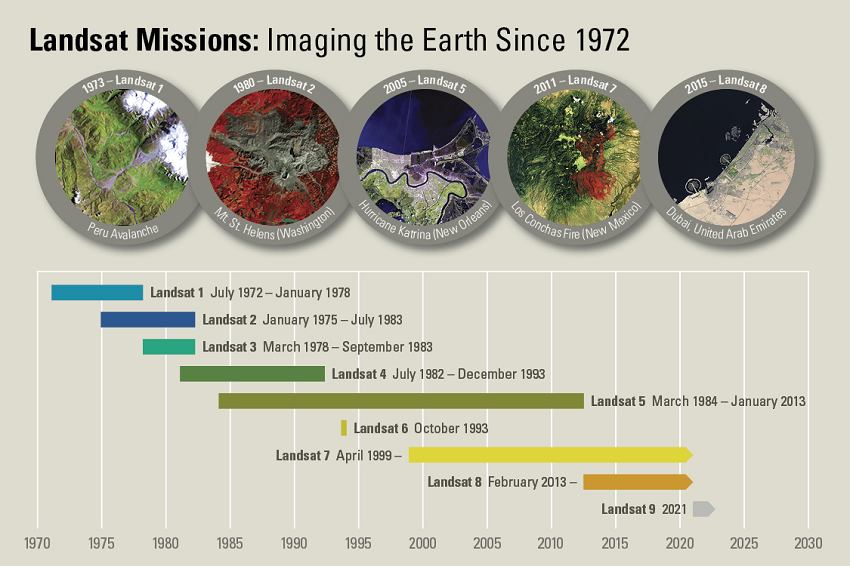
\includegraphics[width=1\linewidth]{2_CAPITULO0/IMG/linea_tiempo_landsat.png}
                        \begin{justify}
                            \textit{Nota.} La línea de tiempo destaca que, desde su inicio en 1972, las misiones Landsat han brindado una secuencia constante de datos que revelan las transformaciones de la Tierra, apoyando así diversas investigaciones y evidenciando su desarrollo en la vigilancia ambiental global. Tomado de \textcite{USGS2023}.
                        \end{justify}                    
                        \label{landsat_missions}
                    \end{figure}



                    La idea de crear un satélite de observación civil surgió en la década de 1960, lográndose el 23 de julio de 1972 con el lanzamiento de ERTS-1, luego renombrado Landsat 1. A este le siguieron varias versiones, siendo Landsat 5 el que estableció un récord por ser el satélite de observación terrestre en funcionamiento más longevo.
                
                \paragraph{Adquisiciones satelitales}
                    Tanto Landsat 8 como Landsat 9 orbitan la Tierra a una altitud de 705 km, completando una órbita en 99 minutos y pasando por cualquier punto de la Tierra cada 16 días. Entre los dos satélites, se agregan más de 1,500 escenas al archivo USGS diariamente. Landsats 4, 5 y 7 siguieron la misma órbita, mientras que Landsats 1, 2 y 3 tenían una altitud de 920 km \autocite{USGS2023}.
                
                \paragraph{Sensores y designaciones de bandas}
                    Los sensores han variado a lo largo de las versiones de Landsat. Desde el Multispectral Scanner (MSS) en los primeros Landsats hasta el Operational Land Imager (OLI) y el Thermal Infrared Sensor (TIRS) en los Landsats más recientes.
                
                    \begin{table}[H]
                        \caption{\doublespacing \\ \textit{Comparación y visualización de bandas y longitudes de onda de sensores Landsat mediante Spectral Viewer del U.S. Geological Survey.}}
                        \begin{spacing}{8}
                            \fontsize{8pt}{2pt}\selectfont  
                            \begin{tabularx}{\linewidth}{P{3cm}*{10}{c}} 
                                \toprule
                                \textbf{Designaciones de banda} & \multicolumn{2}{c}{\textbf{L8-9 OLI/TIRS}} & \multicolumn{2}{c}{\textbf{L7 ETM+}} & \multicolumn{2}{c}{\textbf{L4-5 TM}} & \multicolumn{2}{c}{\textbf{L4-5 MSS*}} & \multicolumn{2}{c}{\textbf{L1-3 MSS*}} \\
                                \midrule
                                & B & Longitud & B & Longitud & B & Longitud & B & Longitud & B & Longitud \\
                                \midrule
                                Costera/Aerosol & 1 & 0.43–0.45 & -- & -- & -- & -- & -- & -- & -- & -- \\
                                Azul & 2 & 0.45–0.51 & 1 & 0.45–0.52 & 1 & 0.45–0.52 & -- & -- & -- & -- \\
                                Verde & 3 & 0.53–0.59 & 2 & 0.52–0.60 & 2 & 0.52–0.60 & 1 & 0.5–0.6 & 4 & 0.5–0.6 \\
                                Pancromática** & 8  & 0.50–0.68 & 8 & 0.52–0.90 & -- & -- & -- & -- & -- & -- \\
                                Rojo & 4 & 0.64–0.67 & 3 & 0.63–0.69 & 3 & 0.63–0.69 & 2 & 0.6–0.7 & 5 & 0.6–0.7 \\
                                Infrarrojo cercano & 5 & 0.85–0.88 & 4 & 0.77–0.90 & 4 & 0.76–0.90 & 3 & 0.7–0.8 & 6 & 0.7–0.8 \\
                                Infrarrojo cercano & -- & -- & -- & -- & -- & -- & 4 & 0.8–1.1 & 7 & 0.8–1.1 \\
                                Cirrus & 9 & 1.36–1.38 & -- & -- & -- & -- & -- & -- & -- & -- \\
                                Infrarrojo corto-1 & 6 & 1.57–1.65 & 5 & 1.55–1.75 & 5 & 1.55–1.75 & -- & -- & -- & -- \\
                                Infrarrojo corto-2 & 7 & 2.11–2.29 & 7 & 2.09–2.35 & 7 & 2.08–2.35 & -- & -- & -- & -- \\
                                Térmico & 10 T1 & 10.60–11.19 & 6 T2 & 10.40–12.50 & 6 T2 & 10.40–12.50 & -- & -- & -- & -- \\
                                Térmico & 11 T1 & 11.50–12.51 & -- & -- & -- & -- & -- & -- & -- & -- \\
                                \bottomrule
                            \end{tabularx}
                        \end{spacing}
                        \vspace{1\baselineskip}
                        \textit{Nota.} Hay observaciones que se debe tener en cuenta. Adapatado de \textcite{Landsat2023}. \\
                            * Adquirido a 80 metros, remuestreado a 60 metros. \\
                            ** 15 metros (pancromático). \\
                            T1 = Térmico (adquirido a 100 metros, remuestreado a 30 metros). \\
                            T2 = Térmico (adquirido a 120 metros, remuestreado a 30 metros). 
                        \label{BandasLandsat}
                    \end{table}
                
                    \begin{table}[H]
                        \caption{\doublespacing \\ \textit{Comparación de sensores Landsat}}
                        \begin{spacing}{8}
                            \fontsize{8pt}{2pt}\selectfont  
                            \begin{tabularx}{\linewidth}{*{6}{c}P{3.5cm}} 
                                \toprule
                                \textbf{Banda} & \textbf{L8–9 OLI/TIRS} & \textbf{L7 ETM+} & \textbf{L4–5 TM} & \textbf{L4–5 MSS} & \textbf{L1–3 MSS} & \multicolumn{1}{c}{\textbf{Uso}} \\
                                \midrule
                                Costero/Aerosol & Banda 1 & -- & -- & -- & -- & Observaciones costeras y detección de aerosoles. \\
                                Azul & Banda 2 & Banda 1 & Banda 1 & -- & -- & Mapeo batimétrico y discriminación suelo/vegetación. \\
                                Verde & Banda 3 & Banda 2 & Banda 2 & Banda 1 & Banda 4 & Evaluación de la vegetación. \\
                                Rojo & Banda 4 & Banda 3 & Banda 3 & Banda 2 & Banda 5 & Identificación de vegetación y suelos. \\
                                Infrarrojo Cercano & Banda 5 & Banda 4 & Banda 4 & Banda 3 & Banda 6 & Análisis y detección de vegetación. \\
                                & -- & -- & -- & Banda 4 & Banda 7 &  \\
                                Infrarrojo Onda Corta-1 & Banda 6 & Banda 5 & Banda 5 & -- & -- & Análisis de humedad y detección de incendios. \\
                                Infrarrojo Onda Corta-2 & Banda 7 & Banda 7 & Banda 7 & -- & -- & Detección de incendios y análisis de humedad. \\
                                Panchromático & Banda 8 & Banda 8 & -- & -- & -- & Mejora de resolución en imágenes multiespectrales. \\
                                Cirrus & Banda 9 & -- & -- & -- & -- & Detección de nubes cirrus. \\
                                Térmico & Banda 10 & Banda 6 & Banda 6 & -- & -- & Mapeo de temperatura y estimación de humedad.
                                \\
                                \bottomrule
                            \end{tabularx}
                        \end{spacing}
                        \vspace{1\baselineskip}
                        \textit{Nota.} Se observa una tendencia en el uso de diferentes bandas para monitorear vegetación, analizar humedad, clima y mejorar la resolución de imágenes. Adaptado de \textcite{Landsat2023}.
                        \label{UsoLandsat}
                    \end{table}
                
                \paragraph{Aplicaciones de los datos Landsat}
                    Los datos de Landsat respaldan una amplia gama de aplicaciones, desde investigación del cambio global hasta seguimiento de derrames de petróleo y monitoreo de contaminación por residuos mineros.
                    

            \subsubsection{Landsat MSS}
                El Multispectral Scanner (MSS) fue el primer sensor de Landsat, utilizado en las misiones Landsat 1 a 5. Este sensor capturaba imágenes en cuatro bandas espectrales, con una resolución espacial de 79 metros para las bandas 1 a 4 y de 185 metros para la banda 5. Aunque el MSS fue reemplazado por el Thematic Mapper (TM) en Landsat 4, 5 y 7, sus datos siguen siendo valiosos para estudios de largo plazo y análisis de series temporales \autocite{landsat_legacy}.
                \paragraph{Landsat 1 (ERTS-1) y su MSS}
                    Originalmente denominado Earth Resources Technology Satellite (ERTS-1), fue lanzado el 23 de julio de 1972. El satélite llevaba a bordo el MSS, un sistema de escaneo multiespectral que capturaba imágenes en cuatro bandas espectrales (verde, rojo, y dos infrarrojas cercanas) con una resolución espacial de 80 metros . Esta tecnología permitía detectar y analizar cambios en el uso del suelo y la vegetación con mayor detalle que los sistemas anteriores.
                    Durante su operación, Landsat 1 experimentó problemas técnicos, como la falla de una de sus grabadoras de cinta de video en agosto de 1972, seguida por la segunda en 1974, lo que limitó la capacidad de grabar datos de manera continua . A pesar de estos desafíos, el MSS proporcionó imágenes claras y precisas que demostraron ser esenciales para una variedad de aplicaciones científicas y de gestión de recursos.

                    \begin{figure}[H] 
                        \caption{\doublespacing \\ \textit{Primera imagen terrestre sin nubes adquirida por el Landsat 1 MSS, 25 de julio de 1972.}} 
                        \centering
                        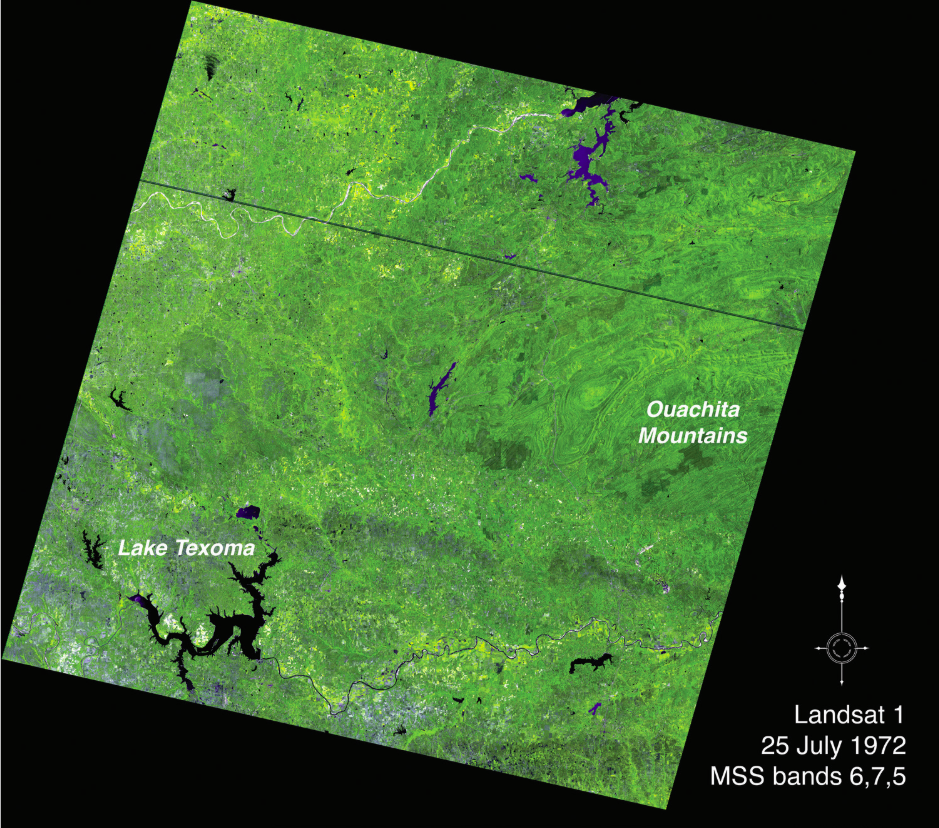
\includegraphics[width=1\linewidth]{2_CAPITULO2/IMG/landsat1.png}
                        \begin{justify}
                            \textit{Nota.} Imagen sin nubes del sistema MSS de Landsat 1 mostrando las Montañas Ouachita en el sureste de Oklahoma. Tomado de \textcite{landsat_legacy}.
                        \end{justify}                    
                        \label{landsat1}
                    \end{figure}

                \paragraph{Landsat 2}
                    Lanzado el 22 de enero de 1975, fue diseñado de manera similar a Landsat 1 y continuó la misión de su predecesor con mejoras en la recopilación y manejo de datos . Landsat 2 también estaba equipado con el MSS, que siguió siendo el instrumento principal para la recolección de datos. A lo largo de su misión, Landsat 2 recopiló una vasta cantidad de datos MSS, aunque enfrentó problemas similares con sus grabadoras de cinta, lo que eventualmente afectó su capacidad operativa.

                    \begin{figure}[H] 
                        \caption{\doublespacing \\ \textit{Fondos de escenas de USGS EROS MSS archivados en 1975 por Landsat 1 y Landsat 2.}} 
                        \centering
                        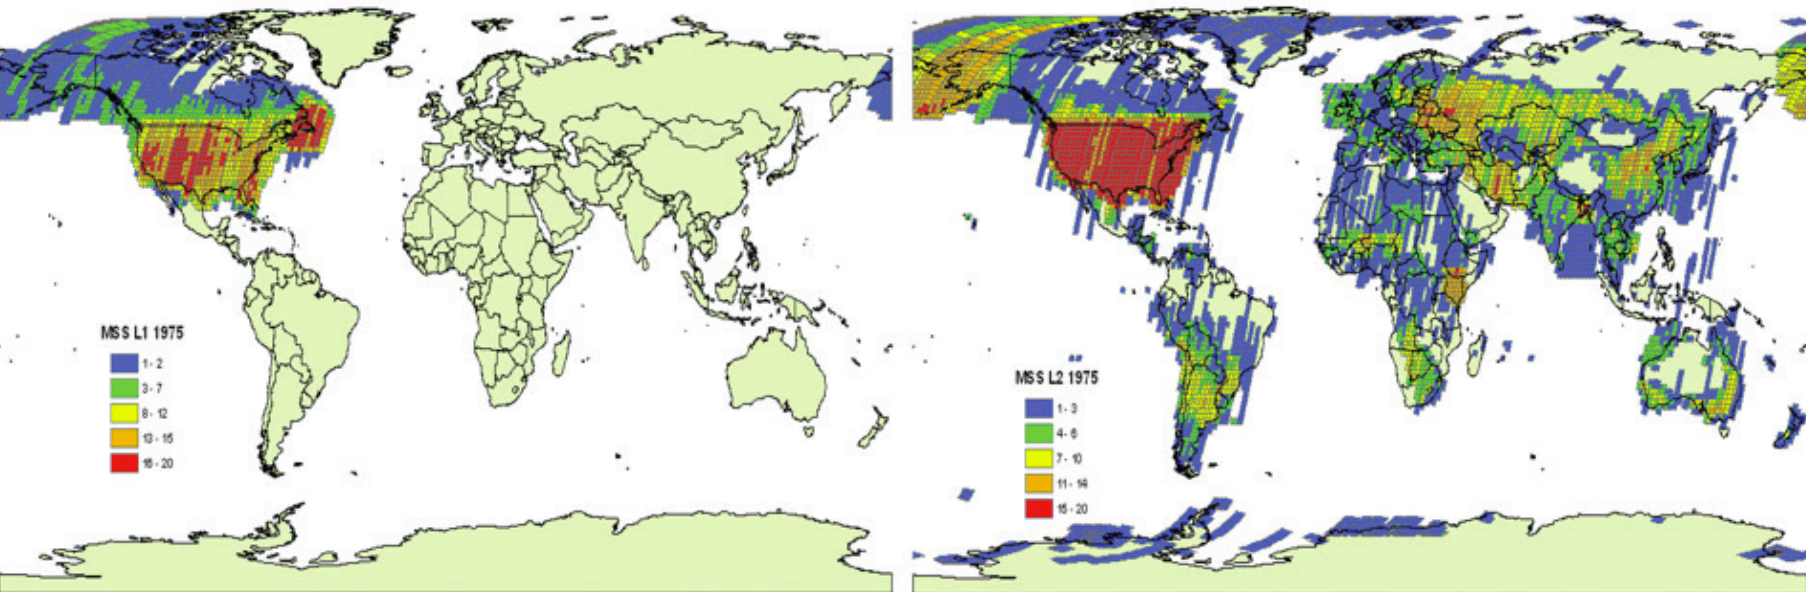
\includegraphics[width=1\linewidth]{2_CAPITULO2/IMG/landsat2.png}
                        \begin{justify}
                            \textit{Nota.} Comparación de las escenas MSS archivadas de Landsat 1 y 2 en 1975, mostrando la cantidad y distribución de datos recopilados. Tomado de \textcite{landsat_legacy}.
                        \end{justify}                    
                        \label{landsat2}
                    \end{figure}

                \paragraph{Landsat 3}
                    Lanzado el 5 de marzo de 1978, introdujo algunas mejoras en el MSS, incluyendo una banda infrarroja térmica para la recolección de datos nocturnos . Sin embargo, el satélite enfrentó varios problemas técnicos que afectaron su rendimiento. La calidad de los componentes del MSS era inferior a la de los satélites anteriores, lo que resultó en fallas recurrentes y una disminución en la calidad de los datos . A pesar de estos problemas, Landsat 3 contribuyó con valiosos datos MSS hasta su retiro en 1983.
                    
                    \begin{figure}[H] 
                        \caption{\doublespacing \\ \textit{Inicio de los problemas de inicio de línea Landsat 3 MSS.}} 
                        \centering
                        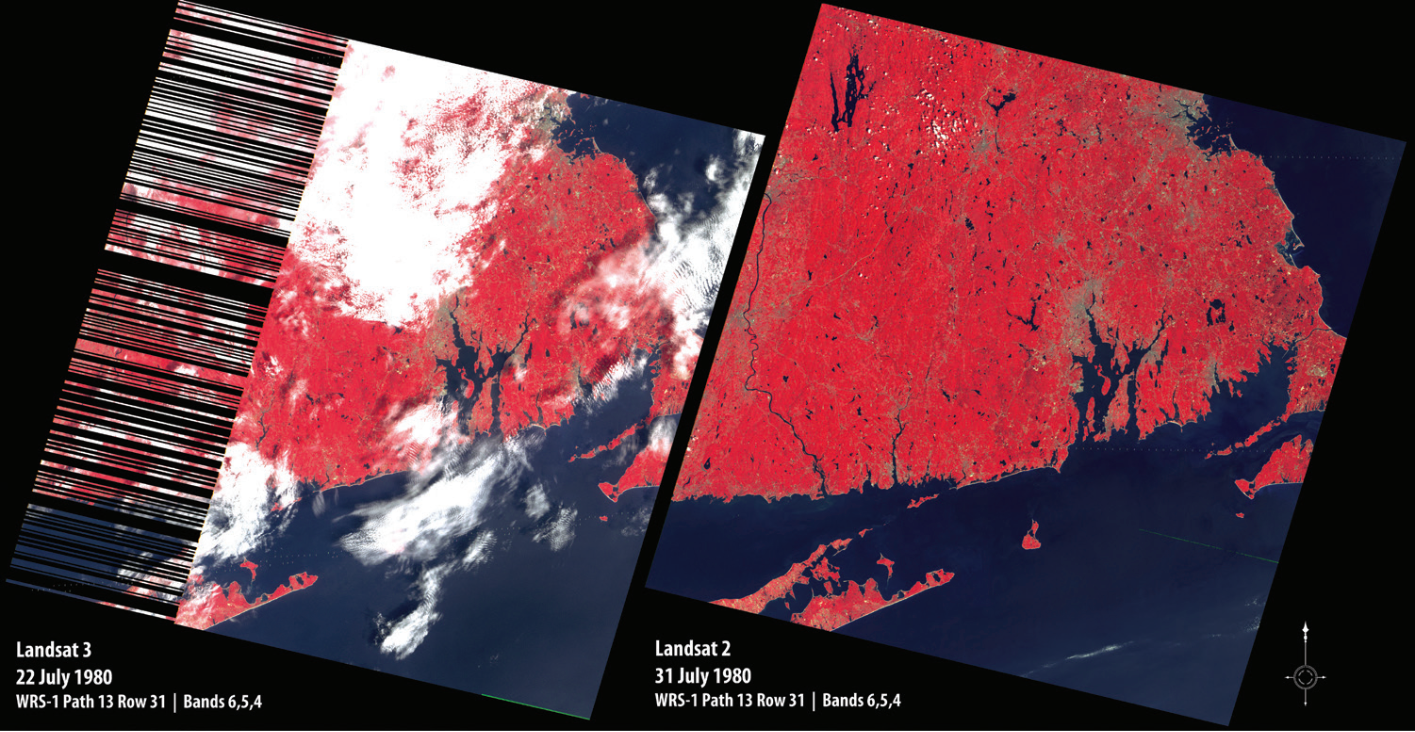
\includegraphics[width=1\linewidth]{2_CAPITULO2/IMG/landsat3.png}
                        \begin{justify}
                            \textit{Nota.} Imagen que muestra los problemas de inicio de línea del MSS de Landsat 3 en comparación con una imagen MSS de Landsat 2. Tomado de \textcite{landsat_legacy}.
                        \end{justify}                    
                        \label{landsat3}
                    \end{figure}

                \paragraph{Landsat 4}
                    Lanzado el 16 de julio de 1982, marcó una evolución significativa con la introducción del Thematic Mapper (TM), aunque el MSS continuó operando como un sensor secundario​​ . Landsat 4 enfrentó desafíos técnicos con su sistema de transmisión de datos, lo que limitó inicialmente la cantidad de datos MSS que pudo recolectar. No obstante, cuando la capacidad de transmisión se estabilizó, Landsat 4 proporcionó una cobertura casi completa a través de TDRS (Tracking and Data Relay Satellite) hasta 1987.

                    \begin{figure}[H] 
                        \caption{\doublespacing \\ \textit{Mapas de cobertura anual de Landsat 4 MSS (1982-1992).}} 
                        \centering
                        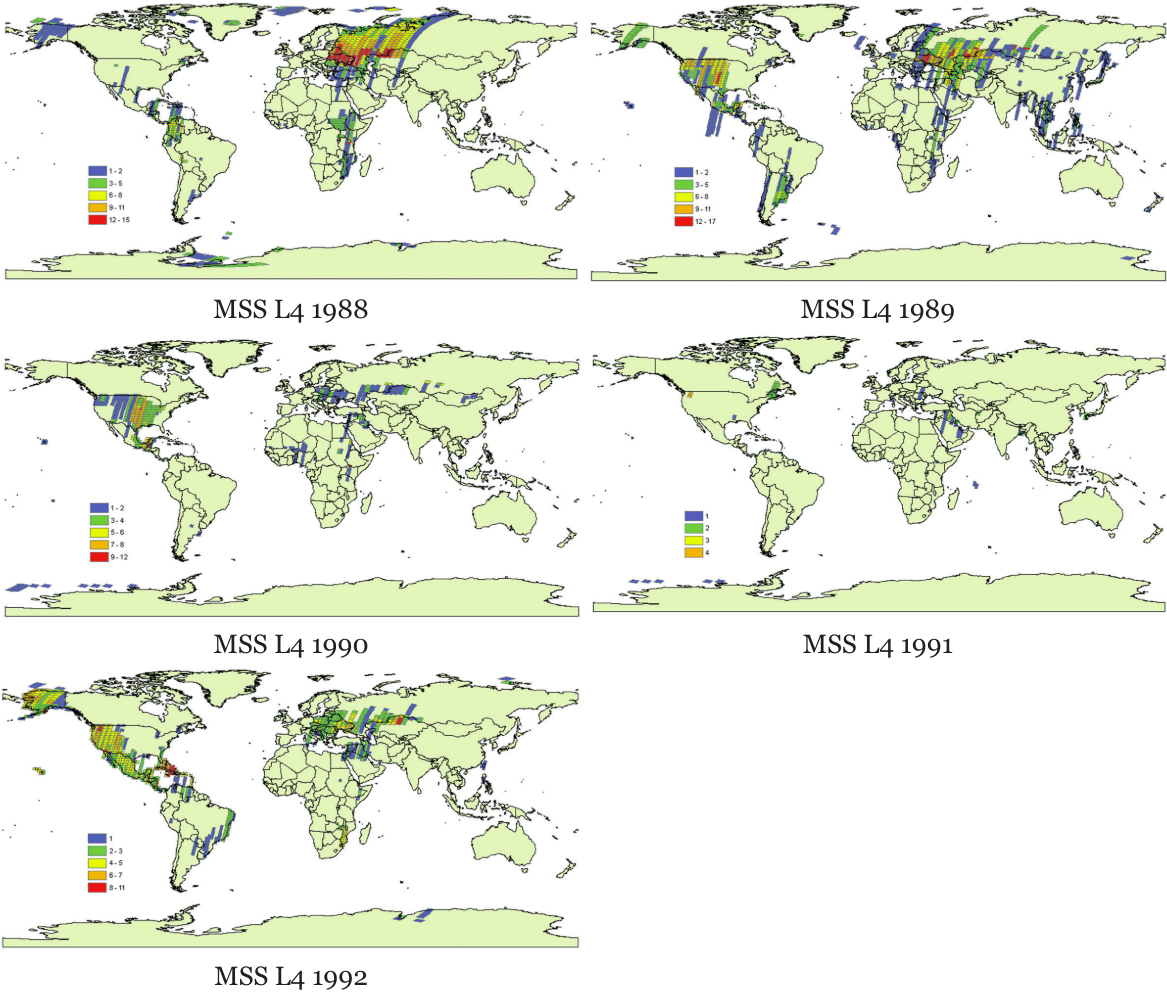
\includegraphics[width=1\linewidth]{2_CAPITULO2/IMG/landsat4.png}
                        \begin{justify}
                            \textit{Nota.} Mapas de cobertura anual del MSS de Landsat 4, mostrando la cobertura geográfica durante su operación. Tomado de \textcite{landsat_legacy}.
                        \end{justify}                    
                        \label{landsat4}
                    \end{figure}

                \paragraph{Landsat 5}
                    Lanzado el 1 de marzo de 1984, es conocido por su longevidad, operando mucho más allá de su vida útil diseñada . Al igual que Landsat 4, Landsat 5 estaba equipado tanto con el TM como con el MSS. Aunque el MSS dejó de ser el sensor principal, continuó recolectando datos valiosos hasta mediados de la década de 1990. Landsat 5 es reconocido por el Guinness World Records como el satélite de observación de la Tierra más duradero en la historia.

                    \begin{figure}[H] 
                        \caption{\doublespacing \\ \textit{Mapas de cobertura anual de Landsat 5 MSS (1984-2007).}} 
                        \centering
                        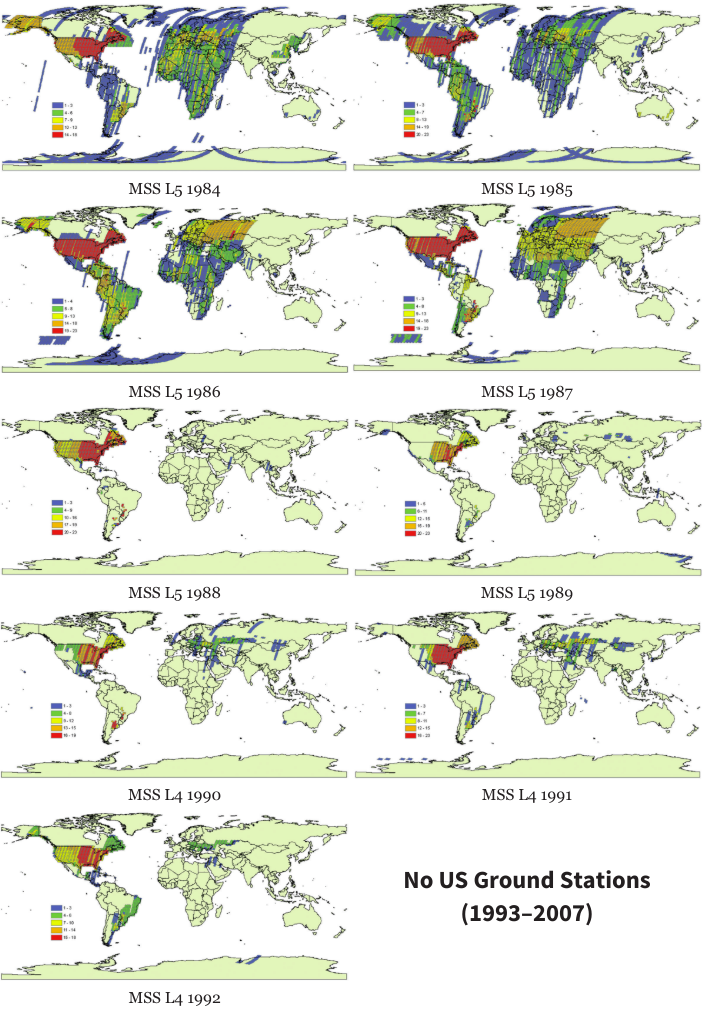
\includegraphics[width=0.9\linewidth]{2_CAPITULO2/IMG/landsat5.png}
                        \begin{justify}
                            \textit{Nota.} Mapas de cobertura anual del MSS de Landsat 5, mostrando la cobertura geográfica durante su operación. Tomado de \textcite{landsat_legacy}.
                        \end{justify}                    
                        \label{landsat5}
                    \end{figure}

                \paragraph{Fechas del Landsat MSS}
                    Las fechas operativas de los sensores MSS de Landsat pueden parecer confusas debido a las múltiples fases de operación y reactivación. El sensor MSS del Landsat cubrió el período desde 1972 hasta 1999, reflejando el uso operativo en los satélites Landsat 1 hasta Landsat 5. En el caso del Landsat 5 MSS, estuvo operativo hasta 2012 porque, aunque dejó de ser la carga principal a finales de los años 90, se reactivó temporalmente en 2012 para llenar brechas de datos antes de la desactivación final del satélite. La reactivación en 2012 se debió a la suspensión de la recopilación de datos TM a finales de 2011, lo que llevó a la reanudación rutinaria de la adquisición MSS hasta diciembre de 2012.

            \subsubsection{Landsat TM}
                El Landsat Thematic Mapper (TM) es un sensor clave en la historia de la observación de la Tierra, destacándose por sus mejoras significativas en resolución espacial y espectral en comparación con sus predecesores. Diseñado para captar imágenes multiespectrales, el TM está equipado con bandas espectrales que cubren desde el azul hasta el infrarrojo térmico, permitiendo una amplia gama de aplicaciones en monitoreo ambiental, gestión de recursos naturales y estudios científicos \autocite{landsat_legacy}.

                \paragraph{Landsat 4}
                    Fue lanzado el 16 de julio de 1982, representando un avance significativo en la teledetección debido a la inclusión del sensor Thematic Mapper (TM). A pesar de sus innovaciones, Landsat 4 enfrentó varios desafíos operacionales desde el inicio, incluyendo fallos en los transmisores de banda X, lo que limitó la capacidad de transmisión de datos del TM hasta que se estableció una conexión a través del sistema de satélites de retransmisión de datos (TDRSS).
                    
                    - \textbf{Problemas de comunicación:} Poco después del lanzamiento, Landsat 4 experimentó fallos en sus transmisores de banda X, dificultando la transmisión de imágenes TM. El lanzamiento del satélite TDRS-E permitió eventualmente la transmisión de datos del TM, aunque con cobertura limitada.
                    
                    - \textbf{Fallos en paneles solares:} En 1983, Landsat 4 perdió el 50\% de su capacidad de generación de energía debido a fallos en los paneles solares. Este problema limitó las operaciones del satélite, afectando su capacidad de recopilación de datos.

                    \begin{figure}[H] 
                        \caption{\doublespacing \\ \textit{Imagen de prueba del Thematic Mapper descargada vía TDRS-E el 12 de agosto de 1983.}} 
                        \centering
                        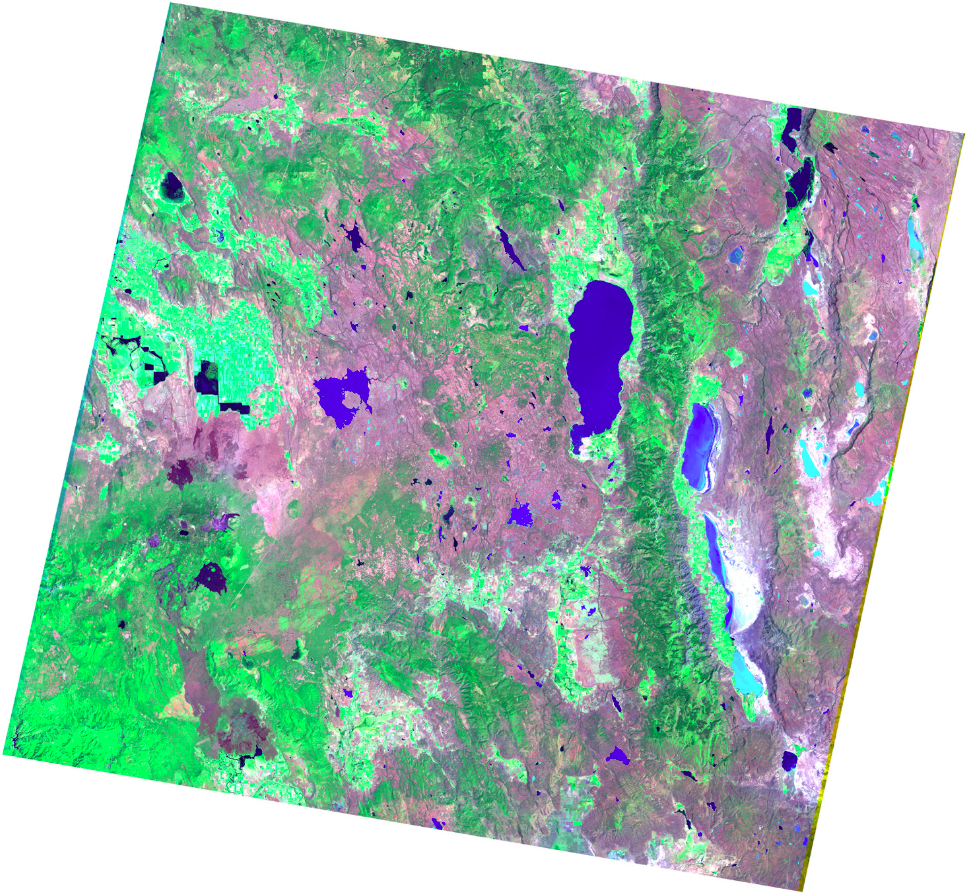
\includegraphics[width=1\linewidth]{2_CAPITULO2/IMG/landsat4_tm.png}
                        \begin{justify}
                            \textit{Nota.} Se muestra un área alrededor de la frontera California/Oregón, incluyendo Goose Lake, Clear Lake National Refuge, Lava Beds National Monument y Modoc National Forest (TM Bandas 7, 4, 2​). Tomado de \textcite{landsat_legacy}.
                        \end{justify}                    
                        \label{landsat4_tm}
                    \end{figure}

                \paragraph{Landsat 5}
                    Fue lanzado el 1 de marzo de 1984, y se destacó por su longevidad operativa, superando significativamente su vida útil de diseño inicial de tres años. Este satélite continuó recopilando datos hasta 2013, estableciendo un récord como la misión satelital de observación de la Tierra más duradera.

                    - \textbf{Desempeño del TM:} A lo largo de su misión, Landsat 5 proporcionó datos de alta calidad gracias al sensor TM, a pesar de enfrentar problemas de comunicación y fallos técnicos. La redundancia en los sistemas críticos y una mayor capacidad de combustible contribuyeron a su longevidad.

                    - \textbf{Innovaciones y aplicaciones:} Las mejoras en resolución espectral y radiométrica del TM permitieron aplicaciones avanzadas en clasificación de tierras y monitoreo ambiental. Estudios realizados con los datos del TM demostraron mejoras significativas en la precisión de clasificación, aunque la resolución espacial mejorada del TM no siempre resultó en mejoras proporcionales en todas las aplicaciones.

                    \begin{figure}[H] 
                        \caption{\doublespacing \\ \textit{Sub-sección de una de las primeras imágenes registradas por el Thematic Mapper de Landsat 5.}} 
                        \centering
                        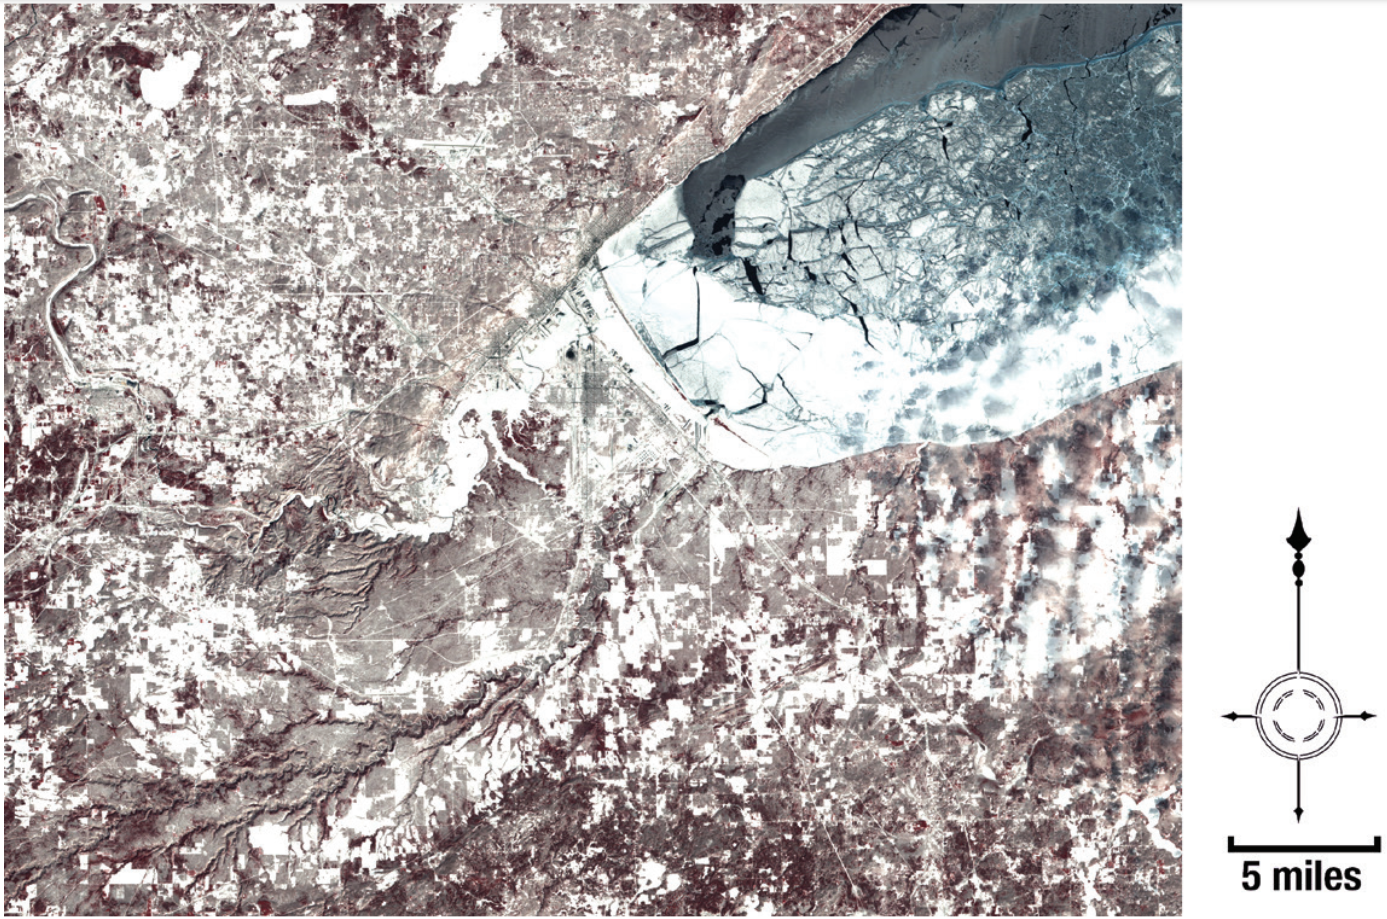
\includegraphics[width=1\linewidth]{2_CAPITULO2/IMG/landsat5_tm.png}
                        \begin{justify}
                            \textit{Nota.} Se muestra Duluth, Minnesota y el rompimiento del hielo en el Lago Superior, adquirida el 6 de marzo de 1984​. Tomado de \textcite{landsat_legacy}.
                        \end{justify}                     
                        \label{landsat5_tm}
                    \end{figure}

            \subsubsection{Armonización de imágenes en Teledetección}
                La armonización se refiere al ajuste radiométrico y geométrico de imágenes de múltiples sensores para garantizar la confiabilidad en teledetección \autocite{ichikawa2022development}. A medida que aumenta la disponibilidad de datos de teledetección, es esencial normalizar imágenes con propiedades radiométricas variables para mosaicos coherentes \autocite{langheinrich2017enhanced}. Además, implica alinear datos de diferentes fuentes para interpretaciones uniformes, utilizando modelos específicos como Fiware \autocite{vosinakis2022data}. Sin embargo, al estudiar la temperatura de la superficie terrestre, la armonización enfrenta desafíos debido a sesgos entre diferentes satélites \autocite{adeniran2022cross}.
                
            \subsubsection{Armonización geométrica de datos de Teledetección}
                Los datos de teledetección a menudo presentan desafíos inherentes. Uno de los principales es la falta de alineación perfecta entre imágenes, lo que da lugar a lo que se conoce como desajustes espaciales o misregistrations \autocite{storey2016note, wolfe2002achieving, yan2018sentinel}. Estos desajustes pueden oscilar desde sub-píxeles hasta unos pocos píxeles.
                
                \paragraph{Causas de desalineaciones}
                    Estos desajustes pueden ser atribuidos a diversas causas, desde la densidad desigual de puntos de control en tierra, el uso de conjuntos de datos de referencia desiguales, hasta problemas en el software de preprocesamiento de los proveedores o movimientos no modelados del sensor \autocite{storey2016note}. Estos desajustes, si no se corrigen, pueden afectar gravemente productos derivados, como clasificaciones de imágenes y detección de cambios.
                    
                \paragraph{Proceso de armonización}
                    La armonización geométrica tiene como objetivo abordar y corregir estas heterogeneidades espaciales. Se compone de dos fases principales: (1) la corrección de misregistrations, y (2) el remuestreo y reproyección de los datos \autocite{roy2000impact}. Sin embargo, corregir estos desajustes no es una tarea sencilla. Las imágenes pueden haber sido adquiridas en diferentes ángulos, fechas, y horarios, lo que complica aún más el proceso de armonización.
                    
                \paragraph{Resampling y Pan-sharpening}
                    A pesar de los desafíos, se han desarrollado técnicas para adaptar diferentes cuadrículas de píxeles mediante remuestreo espacial o pan-sharpening \autocite{ghassemian2016review, javan2021review, li2017pixel}. Estas técnicas están implementadas en varios paquetes de software de código abierto.
                    
                \paragraph{Técnicas de co-registración}
                    Las técnicas de co-registración son esenciales para alinear correctamente las imágenes. Estas técnicas se pueden clasificar en dos categorías principales: basadas en características y basadas en intensidad \autocite{zitova2003image}. Mientras que las primeras se centran en características notables en las imágenes, como edificios o carreteras, las segundas se basan en patrones de valores de grises. Ambas técnicas ofrecen sus propios beneficios y desafíos. 
                    
                \paragraph{Necesidad de un método universal}
                    Dada la diversidad y complejidad de los datos de teledetección, es esencial contar con un método de co-registración que sea universalmente aplicable \autocite{chen2003mutual}. Este método debería ser capaz de manejar desajustes técnicos entre múltiples sensores y desafíos presentados por paisajes y atmósferas cambiantes.

            \subsubsection{Armonización espectral de datos de Teledetección}
                Los sensores de teledetección óptica se caracterizan por presentar diversos bandas espectrales, abarcando no solo el espectro electromagnético visible (VIS, ~400 – 700 nm), sino también el infrarrojo cercano (NIR, ~750 – 1000 nm) y el infrarrojo de onda corta (SWIR, ~1000 – 2500 nm). Estos sensores facilitan la diferenciación de materiales superficiales y permiten identificar ciertas propiedades del cobertura terrestre o composiciones atmosféricas.
                
                \paragraph{Discrepancias espectrales entre sensores}
                    Aunque satélites de Observación de la Tierra (EO) como Landsat (NASA) o Sentinel-2 (ESA) suelen diseñarse con características espectrales similares para garantizar la comparabilidad a largo plazo, aún existen discrepancias en el número de bandas y las respuestas espectrales de cada sensor \autocite{drusch2012sentinel}.
                    
                \paragraph{Objetivo de la armonización espectral}
                    La armonización espectral busca transformar la información espectral de un sensor al dominio espectral de otro, con el fin de estandarizar el número de bandas y reducir inconsistencias entre imágenes de múltiples sensores, facilitando así análisis y flujos de trabajo posteriores.
                    
                \paragraph{Técnicas existentes}
                    Existen técnicas basadas en relaciones estadísticas de bandas equivalentes de múltiples sensores para lograr una transformación espectral \autocite{chastain2019empirical, claverie2018harmonized, flood2014continuity, roy2016characterization}. Sin embargo, estas técnicas están limitadas a bandas con equivalentes directos entre sensores, lo que deja un potencial no aprovechado en regiones espectrales como el borde rojo \autocite{filella1994red}.
                    
                \paragraph{Necesidad de avances metodológicos}
                    Es fundamental avanzar en las técnicas existentes de armonización espectral para estimar con precisión la información espectral faltante y reducir los errores de armonización que varían espacialmente. Además, es esencial evaluar el rendimiento de diferentes técnicas de armonización y cuantificar los errores de estimación según los materiales superficiales y las longitudes de onda de las bandas estimadas.
                    
            \subsubsection{Normalización y ajuste de datos con aplicación de parámetros BRDF}    

                \paragraph{Fundamentos de la función de distribución bidireccional de reflectancia (BRDF)}
                    En estudios anteriores, la BRDF se estableció como una función esencial que caracteriza cómo la luz es reflejada por las superficies terrestres en varias direcciones. Se observó que las superficies no son Lambertianas, lo que significa que la reflectancia varía con la geometría solar y de observación. Esto es crucial para corregir y comparar datos de reflectancia obtenidos en diferentes momentos y bajo diversas condiciones de iluminación \autocite{roy2016general}.
                \paragraph{Aplicación de parámetros BRDF en la normalización de datos}
                    La práctica de normalizar la reflectancia a través de parámetros BRDF se mostró eficaz para estandarizar las observaciones de Landsat a una vista de nadir. Esto permite mitigar los efectos direccionales y obtener una reflectancia consistente y comparable en el tiempo. Se utilizó un enfoque de c-factor, multiplicando la reflectancia observada por el cociente de la reflectancia modelada, lo que resultó ser poco sensible al tipo de cobertura terrestre y por lo tanto aplicable a todo el registro de Landsat \autocite{roy2016general}.
                \paragraph{Integración de datos TM y ETM+ en modelos BRDF}
                    La integración de datos de los sensores TM y ETM+ en modelos BRDF se abordó para proporcionar una reflectancia ajustada al nadir más consistente. Se descubrió que los parámetros de BRDF de MODIS podían ser aplicados a estos datos, lo que sugiere que las formas de BRDF de diversas superficies terrestres son lo suficientemente similares como para permitir esta aplicación directa, facilitando la generación de NBAR para una amplia gama de aplicaciones de monitoreo terrestre.

                    \begin{table}[H]
                        \caption{\doublespacing \\ \textit{Parámetros BRDF MODIS globales fijos para todas las bandas Landsat.}}
                        \begin{spacing}{8}
                            \fontsize{8pt}{2pt}\selectfont
                            \begin{tabularx}{\linewidth}{P{2.5cm}P{2.6cm}P{4cm}P{2.5cm}P{2.5cm}}
                                \toprule
                                \multicolumn{1}{c}{\textbf{Banda Landsat}} & \multicolumn{1}{c}{\textbf{n}} & \multicolumn{1}{c}{\textbf{fiso}} & \multicolumn{1}{c}{\textbf{fgeo}} & \multicolumn{1}{c}{\textbf{fvol}} \\
                                \midrule
                                1 (azul)               & 15,551,077,545      & 0.0774        & 0.0079        & 0.0372        \\
                                2 (verde)              & 16,362,112,402      & 0.1306        & 0.0178        & 0.0580        \\
                                3 (rojo)               & 16,095,103,393      & 0.1690        & 0.0227        & 0.0574        \\
                                4 (NIR)                & 16,260,280,058      & 0.3093        & 0.0330        & 0.1535        \\
                                5 (1.6µm)              & 16,176,131,413      & 0.3430        & 0.0453        & 0.1154        \\
                                7 (2.1µm)              & 16,149,440,059      & 0.2658        & 0.0387        & 0.0639        \\
                                \bottomrule
                            \end{tabularx}
                        \end{spacing}
                        \vspace{1\baselineskip}
                        \textit{Nota.} La tabla muestra los parámetros BRDF fijos de MODIS para cada banda de Landsat, utilizados en normalización y comparación con datos satelitales; estos parámetros son constantes y globales durante 12 meses en todas las bandas, reflejando la cantidad 'n' de píxeles de alta calidad y sin nieve a 500 m en los espectrales MODIS BRDF, donde 'n' varía según la banda, lo que corresponde a las variaciones en la calidad de parámetros en el producto MODIS BRDF/Albedo (MCD43A2) \autocite{roy2016general}.
                        \label{tab:modis_brdf_parameters}
                    \end{table}
        \subsection{Inteligencia artificial}            
            \subsubsection{Deep learning en el procesamiento de imágenes de Teledetección}
                El deep learning, especialmente en el ámbito de la teledetección, ha emergido como una técnica central y de vanguardia para diversas aplicaciones de visión por computadora. Los investigadores están en constante búsqueda de mejorar el rendimiento de los métodos de deep learning mediante el desarrollo de nuevos diseños arquitectónicos de redes y/o la implementación de técnicas innovadoras, como los mecanismos de atención \autocite{ghaffarian2021effect}. Estos avances han demostrado ser esenciales para mejorar la precisión y eficiencia en el procesamiento de imágenes de teledetección \autocite{wang2022review}.
                
            \subsubsection{Redes neuronales convolucionales (CNN)}
                Las Redes Neuronales Convolucionales, o CNN, son una subcategoría de redes neuronales diseñadas específicamente para manejar datos con una estructura topológica definida. Estas redes son esenciales para el análisis de datos estructurados en series temporales, que se pueden visualizar como una línea continua con intervalos de tiempo uniformes, o imágenes, que se representan como una matriz bidimensional de píxeles. Lo que distingue a las CNN de otras redes neuronales es su uso de la convolución, una operación matemática lineal específica. En lugar de depender únicamente de las multiplicaciones matriciales, las CNN incorporan la operación de convolución en al menos una de sus capas 
                \autocite{Goodfellow2016}.

                \paragraph{Convolución y su aplicación en aprendizaje profundo}0
                    La convolución es una operación matemática esencial en el procesamiento de señales, especialmente en el análisis de imágenes dentro del aprendizaje profundo. Es particularmente relevante en las Redes Neuronales Convolucionales (CNNs) \autocite{Goodfellow2016}. En términos generales, la convolución evalúa cómo se superpone una función con otra cuando una de ellas se desplaza sobre la otra.
                    
                    La operación matemática de la convolución entre dos funciones, $x(a)$ y $w(a)$, se representa como:
                    
                    \begin{equation}
                    s(t) = \int x(a)w(t-a)da
                    \end{equation}
                    
                    Donde $x(a)$ es conocida como la función de entrada y $w(a)$ es el kernel o filtro. El resultado, $s(t)$, es a menudo denominado mapa de características o "feature map". En aprendizaje automático, tanto la función de entrada como el kernel suelen ser matrices multidimensionales o tensores.
                    
                    Para visualizarlo en el contexto de imágenes, consideremos una imagen bidimensional $I$ y un kernel bidimensional $K$:
                    
                    \begin{equation}
                    S(i,j) = \sum_m \sum_n I(m,n)K(i-m,j-n)
                    \end{equation}
                    
                    Donde $I(m,n)$ representa el valor del píxel en la posición $(m,n)$ de la imagen y $K(i-m,j-n)$ es el valor correspondiente del kernel. Dada la propiedad conmutativa de la convolución, esta ecuación también puede expresarse como:
                    
                    \begin{equation}
                    S(i,j) = \sum_m \sum_n I(i+m,j+n)K(m,n)
                    \end{equation}
                    
                    Es importante señalar que, en el ámbito del aprendizaje profundo, a menudo se utiliza una operación similar llamada \textit{correlación cruzada}:
                    
                    \begin{equation}
                    S(i,j) = \sum_m \sum_n I(i+m,j+n)K(m,n)
                    \end{equation}
                    
                    A diferencia de la convolución, en la correlación cruzada no se invierte el kernel.

                    \insertfigure
                        {Una convolución 2-D sin invertir el núcleo}
                        {2_CAPITULO0/IMG/convolucion.png}
                        {En la convolución 2-D un núcleo de 2x2 se desplaza sobre una matriz 4x4, multiplicando y sumando correspondencias sin invertir el núcleo, formando así la matriz de salida, un proceso clave en procesamiento de imágenes y redes neuronales convolucionales. Tomado de \textcite{USGS2023}.} 
                

                \paragraph{Padding}
                    En el contexto de las Redes Neuronales Convolucionales (CNN), el \textit{padding} es un mecanismo crucial que permite mantener la dimensionalidad de una imagen de entrada durante el proceso de convolución. La idea principal detrás del \textit{padding} es añadir ciertos valores alrededor de una matriz de entrada, y estos valores adicionales son comúnmente representados por el símbolo \( p \) \autocite{Goodfellow2016}.

                    Considere una imagen de entrada representada por una matriz \( I \) de dimensiones \( n \times n \). Si aplicamos un kernel (o filtro) de tamaño \( f \times f \) a esta imagen, la matriz resultante (sin aplicar \textit{padding}) tendrá un tamaño de \( n - f + 1 \times n - f + 1 \). Esto se debe a que, durante la operación de convolución, el kernel se desliza sobre la imagen de entrada, y, dependiendo del tamaño del kernel, algunas partes de la imagen no son cubiertas.
                    
                    En la \autoref{padding1}, se ilustra un proceso de convolución donde la matriz de entrada \( I \), de dimensiones \( 5 \times 5 \), se convoluciona con un kernel \( K \) de dimensiones \( 3 \times 3 \). Se utiliza un \textit{padding} \( p \) de valor 0 y un \textit{stride} \( s \) de valor 1, que es el valor comúnmente asumido. A través de esta operación, obtenemos una matriz de salida \( S \) con dimensiones \( 3 \times 3 \), calculadas mediante la fórmula \( 5 - 3 + 1 \times 5 - 3 + 1 \). Específicamente, para la posición \( S(0, 0) \) de la matriz de salida, el valor es 155, determinado por la operación de convolución especificada en la figura. Notamos que, debido a que no hay \textit{padding} (es decir, \( p = 0 \)), la matriz de salida es dos unidades menor en dimensiones que la matriz original.

                    De manera similar, en la \autoref{padding2}, se presenta un cálculo para la posición \( S(0, 1) \) con un resultado de 85.

                    \begin{figure}[H] 
                        \caption{\doublespacing \\ \textit{Cálculo de la convolución de una matriz de entrada \( 5 \times 5 \) con un kernel \( 3 \times 3 \) con \( p = 0 \) y \( s = 1 \)}} 
                        \centering
                        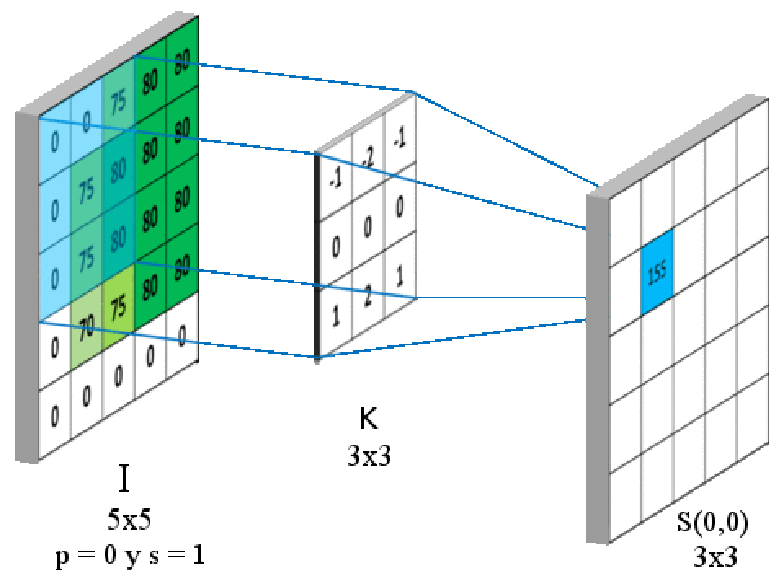
\includegraphics[width=1\linewidth]{2_CAPITULO0/IMG/padding1.png}
                        \begin{justify}
                            \textit{Nota.} La operación genera una matriz de salida de 3x3 donde, por ejemplo, S(0,0) tiene un valor de 155 después de la convolución; la matriz resultante es dos unidades menor que la original por no usar padding. Adaptado de \textcite{Goodfellow2016}.
                        \end{justify}                    
                        \label{padding1}
                    \end{figure}
                    
                    \begin{figure}[H] 
                        \caption{\doublespacing \\ \textit{ Cálculo de la convolución para la posición \( S(0, 1) \) en la matriz de salida.}} 
                        \centering
                        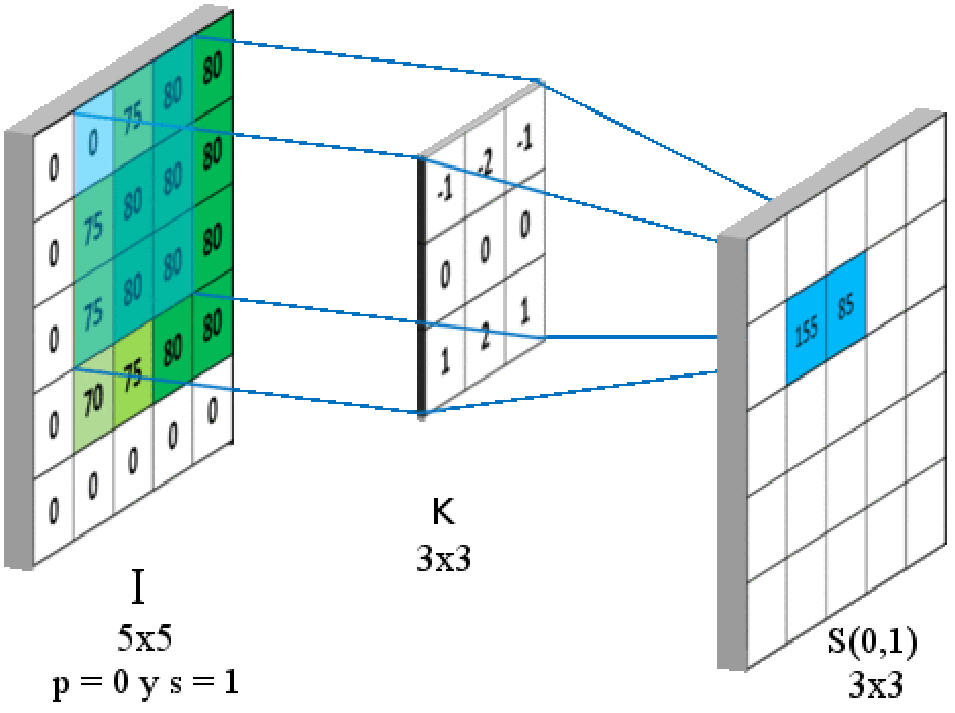
\includegraphics[width=1\linewidth]{2_CAPITULO0/IMG/padding2.png}
                        \begin{justify}
                            \textit{Nota.} La convolución involucra una matriz \(5 \times 5\) y un kernel \(3 \times 3\), resultando en \(S(0,1) = 85\), con líneas azules que representan la transformación. Adaptado de \textcite{Goodfellow2016}.
                        \end{justify}                    
                        \label{padding2}
                    \end{figure}
                    

                    En la mayoría de los casos, \( p = 0 \), pero si \( p > 0 \), la dimensión de la matriz de salida se calcula como:
                    
                    \begin{equation}
                        \text{Dimensión de Salida} = n + 2 \cdot p - f + 1 \times n + 2 \cdot p - f + 1
                    \end{equation}
                    
                    donde \( n \) es la dimensión de la matriz de entrada y \( f \) es la dimensión del filtro.
                    
                    Por ejemplo, en la \autoref{padding3}, considerando un padding \( p = 1 \), una matriz de entrada \( I \) de dimensiones \( 5 \times 5 \), y un filtro de dimensiones \( 3 \times 3 \), la matriz de salida resultante tendrá dimensiones \( 5 \times 5 \), manteniendo así la dimensión espacial de la matriz de entrada.

    
                    \begin{figure}[H] 
                        \caption{\doublespacing \\ \textit{Cálculo de la convolución de una matriz de entrada \( 5 \times 5 \) con un kernel \( 3 \times 3 \) con \( p = 1 \) y \( s = 1 \)}} 
                        \centering
                        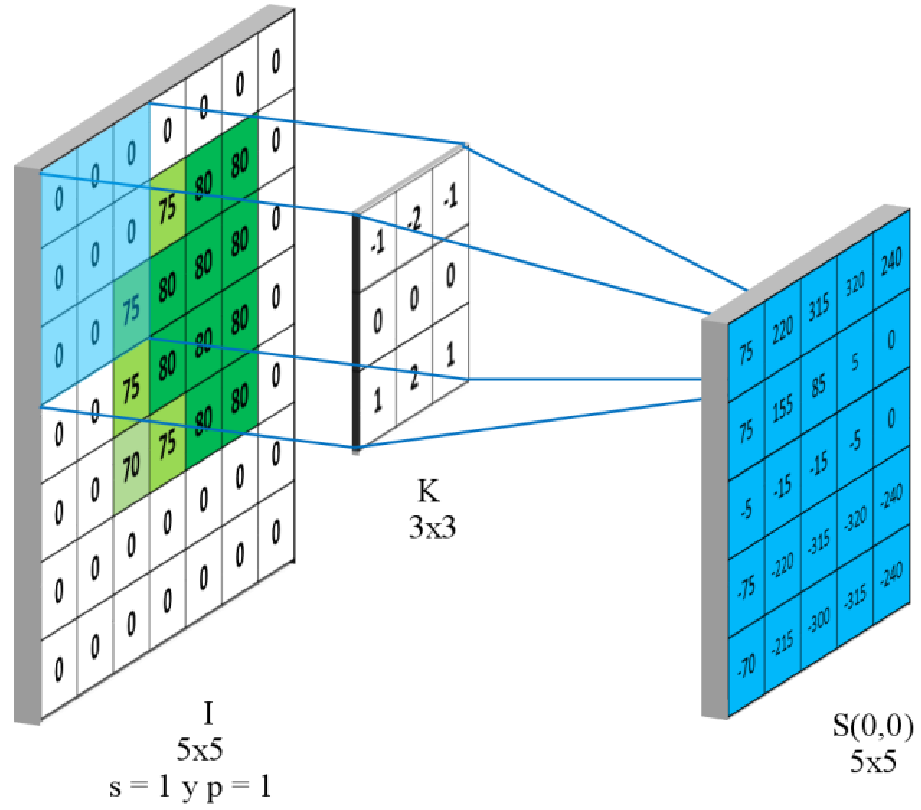
\includegraphics[width=1\linewidth]{2_CAPITULO0/IMG/padding3.png}
                        \begin{justify}
                            \textit{Nota.} \textit{Padding} de \( p=1 \) mantiene dimensiones de la imagen original, esencial para que redes neuronales aprendan patrones locales eficientemente. Adaptado de \textcite{Goodfellow2016}.
                        \end{justify}                    
                        \label{padding3}
                    \end{figure}

                    Las convoluciones pueden clasificarse en:
                    
                    \begin{itemize}
                        \item[-] \textbf{Convoluciones válidas:} No utilizan padding, resultando en una matriz de salida de dimensiones menores.
                        \item[-] \textbf{Convoluciones iguales:} Utilizan padding para asegurar que la matriz de salida tenga las mismas dimensiones que la matriz de entrada.
                    \end{itemize}
                    
                \paragraph{Stride}
                    Anteriormente ha sido denotado como \( s \), representa la cantidad de píxeles que el filtro se moverá durante la operación de convolución. Actualizando la fórmula de la dimensión de salida para incluir el stride, tenemos:
                    
                    \begin{equation}
                        \text{Dimensión de Salida} = \left\lfloor \frac{n + 2 \cdot p - f}{s} + 1 \right\rfloor \times \left\lfloor \frac{n + 2 \cdot p - f}{s} + 1 \right\rfloor
                    \end{equation}
                    
                    Por ejemplo, en la \autoref{stride}, con un stride \( s = 2 \), un padding \( p = 1 \), una matriz de entrada \( I \) de dimensiones \( 5 \times 5 \), y un filtro de dimensiones \( 3 \times 3 \), la matriz de salida resultante tendrá dimensiones \( 3 \times 3 \).
                    
                    \begin{figure}[H] 
                        \caption{\doublespacing \\ \textit{Convolución 2D con Padding de 1 y Stride de 2 en la Posición S(1, 1).}} 
                        \centering
                        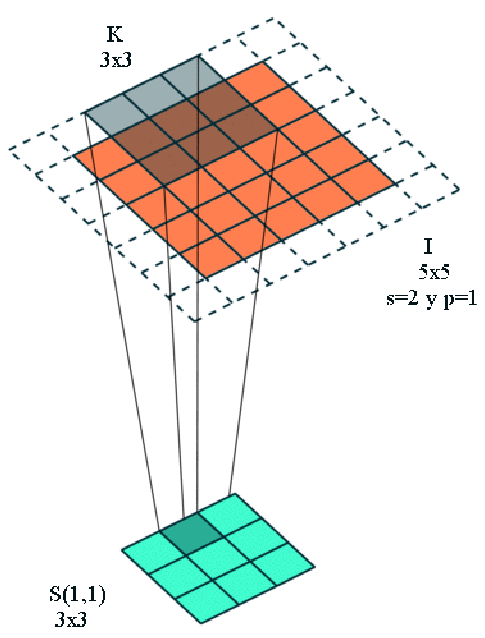
\includegraphics[width=0.8\linewidth]{2_CAPITULO0/IMG/stride.png}
                        \begin{justify}
                            \textit{Nota.} Convolución con stride de 2 y filtro de \(3 \times 3\), desplazando dos píxeles a la vez y padding que preserva información en bordes. Adaptado de \textcite{Goodfellow2016}.
                        \end{justify}                    
                        \label{stride}
                    \end{figure}
                    

            \subsubsection{Tipos de capas en una red neuronal convolucional}
                Las Redes Neuronales Convolucionales emplean una serie de capas específicas que incluyen: Capa de Entrada, Capa Convolucional, Capa de Agrupación, Capa Totalmente Conectada y Capa de Salida. Cada capa tiene funciones específicas y contribuye al rendimiento general de la red.
                \begin{figure}[H] 
                    \caption{\doublespacing \\ \textit{Representación esquemática de una Red Neuronal Convolucional.}} 
                    \centering
                    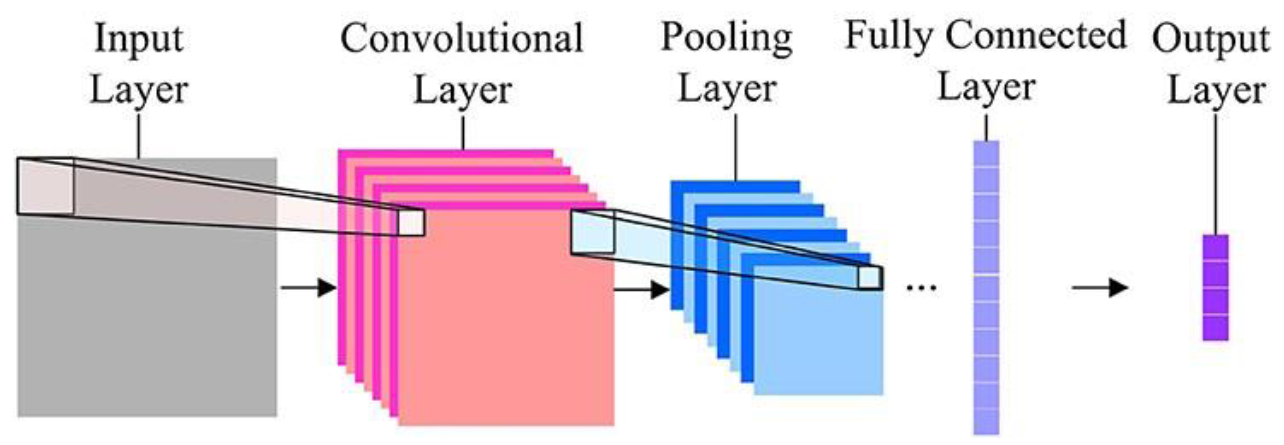
\includegraphics[width=1\linewidth]{2_CAPITULO0//IMG/tipos_capas.png}
                    \begin{justify}
                        \textit{Nota.} La estructura CNN: capas convolucionales detectan patrones y reducen tamaño; una capa conectada integra rasgos para la clasificación final, crucial en procesamiento visual. Adaptado de \textcite{Goodfellow2016}.
                    \end{justify}                    
                    \label{tipos_capas}
                \end{figure}
            
                
                \paragraph{Capa de Convolución}
                    Esta capa realiza operaciones de convolución en la entrada utilizando varios \textit{kernels}. Posteriormente, se agrega un sesgo al resultado y se pasa por una función de activación no lineal como ReLU. Esta función introduce no linealidad tras realizar operaciones lineales en las capas convolucionales. Aunque en el pasado se usaron funciones como tanh y sigmoid, ReLU ha demostrado ser más eficiente en términos de tiempo de entrenamiento y precisión.
                    
                    \begin{figure}[H] 
                        \caption{\doublespacing \\ \textit{Función de activación ReLU.}} 
                        \centering
                        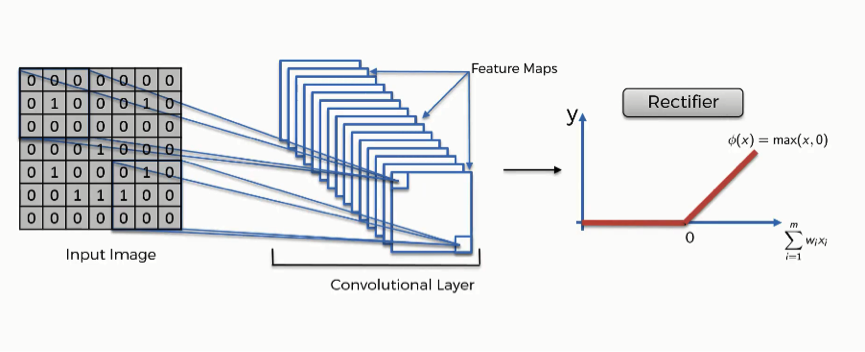
\includegraphics[width=1\linewidth]{2_CAPITULO0//IMG/relu.png}
                        \begin{justify}
                            \textit{Nota.} La función ReLU introduce no linealidad, ayudando a la red a capturar patrones complejos y optimizando el entrenamiento y precisión, evidenciando su ventaja sobre funciones previas como tanh o sigmoid. Tomado de \textcite{Kalita2022}.
                        \end{justify}                    
                        \label{relu}
                    \end{figure}
                
                \paragraph{Capa de agrupación}
                    Destinada a reducir las dimensiones de la entrada, la Capa de Agrupación mejora la eficiencia y robustez de la red. Una técnica popular aquí es el \textit{Max Pooling}, que selecciona el valor máximo de un conjunto específico, en la \autoref{max_pooling} se muestra un ejemplo donde una matriz I de tamaño 6 x 6, con un s igual a 3 y p igual a 0 . Esto es especialmente útil porque no introduce parámetros adicionales y es computacionalmente eficiente.
                    
                    Diversas técnicas de agrupación incluyen:
                    
                    \begin{itemize}
                        \item[-] Agrupación Máxima: \( s_j = \max_{i \in R_j} a_i \)
                        \item[-] Agrupación Promedio: \( s_j = \frac{1}{|R_j|} \sum_{i \in R_j} a_i \)
                        \item[-] Agrupación Estocástica: \( p_j = \frac{a_i}{\sum_{k \in R_j} a_k} \)
                    \end{itemize}

                    \begin{figure}[H] 
                        \caption{\doublespacing \\ \textit{Max-Pooling con padding de 0 y stride de 3 en posición S(0, 0).}} 
                        \centering
                        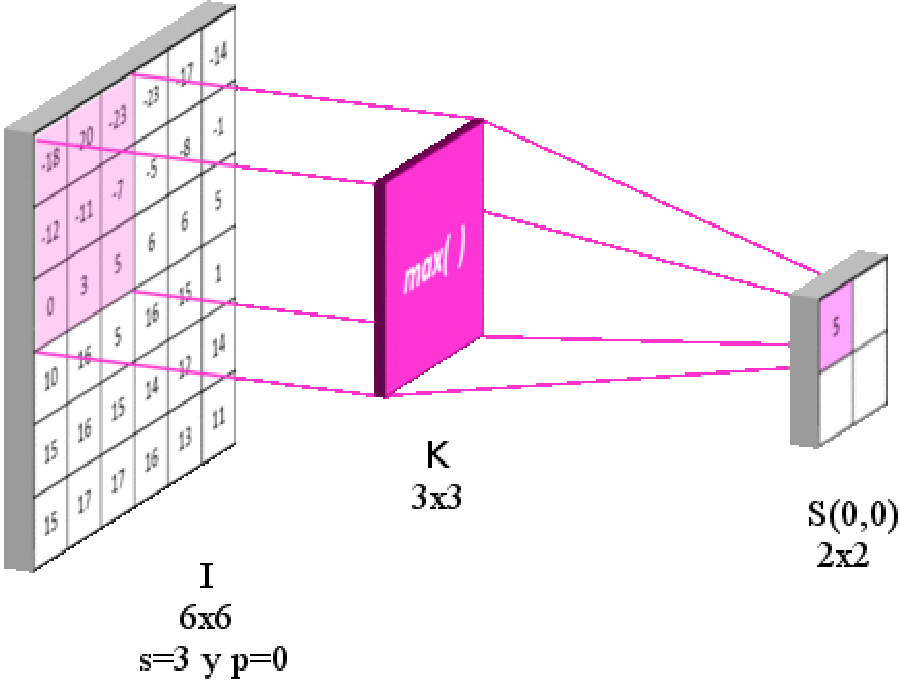
\includegraphics[width=1\linewidth]{2_CAPITULO0//IMG/max_pooling.png}
                        \begin{justify}
                            \textit{Nota.} Max-Pooling con kernel de \(3 \times 3\) y stride de 3 sobre una matriz \(6 \times 6\) extrae máximos locales, resultando en una matriz \(2 \times 2\), compactando información y resaltando características prominentes sin pérdida significativa. Adaptado de \textcite{Goodfellow2016}.
                        \end{justify}                    
                        \label{max_pooling}
                    \end{figure}
                

                \paragraph{Capa totalmente conectada}
                    Después de la agrupación, la entrada se pasa a una capa totalmente conectada que la conecta con la capa de salida, estableciendo conexiones entre todas las unidades \autocite{Goodfellow2016}.
                
                \paragraph{Hiperparámetros}
                    Los hiperparámetros, a diferencia de los parámetros, son valores preestablecidos que determinan cómo se comporta un algoritmo durante el entrenamiento. Estos se definen antes del proceso de aprendizaje y no se adaptan automáticamente durante el mismo \autocite{Goodfellow2016}.
                    
                    Al diseñar arquitecturas de Redes Neuronales Convolucionales (CNN), se consideran diversos hiperparámetros, entre los cuales se encuentran:
                    
                    \begin{itemize}
                        \item[-] \textbf{Tamaño del kernel:} Definido por la dimensión \( f \times f \), se utiliza en la capa convolucional o de agrupación.
                        \item[-] \textbf{Padding:} Indica cuántos píxeles se añaden alrededor de la imagen, normalmente rellenos con cero, para ajustar las dimensiones durante las convoluciones.
                        \item[-] \textbf{Stride:} Define cuántos píxeles se desplaza el kernel durante la convolución.
                        \item[-] \textbf{Número de kernels:} La cantidad de filtros en una capa convolucional.
                        \item[-] \textbf{Número de capas:} El total de capas en una CNN.
                        \item[-] \textbf{Función de activación:} Función no lineal aplicada tras la convolución, comúnmente ReLU, Sigmoid o Tanh.
                    \end{itemize}
                    
                    También se deben considerar hiperparámetros específicos al definir el conjunto de entrenamiento:
                    
                    \begin{itemize}
                        \item[-] \textbf{Muestras de entrenamiento:} Total de ejemplos utilizados en el entrenamiento.
                        \item[-] \textbf{Tamaño del lote (batch size):} Número de ejemplos procesados en una sola iteración de entrenamiento.
                        \item[-] \textbf{Iteraciones:} Total de lotes necesarios para completar una época.
                        \item[-] \textbf{Épocas:} Número de veces que se procesa el conjunto completo de entrenamiento.
                        \item[-] \textbf{Tasa de aprendizaje (\( \varepsilon \)):} Define la magnitud de ajuste de los pesos en función del gradiente de pérdida.
                    \end{itemize}
                    
                    El número de épocas se calcula según la relación:
                    
                    \begin{equation}
                        \text{epochs} = \frac{\text{batch\_size} \times \text{iterations}}{\text{training\_samples}}
                    \end{equation}
                    
                    Existen otros hiperparámetros que se emplean como métodos de regularización:
                    
                    \begin{itemize}
                        \item[-] \textbf{Regularización L2:} Penaliza la magnitud de los pesos para evitar sobreajuste.
                        \item[-] \textbf{Regularización L1:} Similar a L2, pero puede hacer que algunos pesos sean exactamente cero.
                        \item[-] \textbf{Dropout:} Durante el entrenamiento, desactiva aleatoriamente algunas neuronas para prevenir la dependencia excesiva en cualquier neurona individual.
                        \item[-] \textbf{Augmentation:} Amplía el conjunto de entrenamiento al introducir variaciones menores, como rotaciones y escalas, para mejorar la generalización del modelo.
                    \end{itemize}

        \section{Definición de términos}
                       
            \subsection{Armonización de datos}
                Se refiere al proceso de ajustar conjuntos de datos para que sean consistentes entre sí en términos de escala, resolución, calibración y geometría. En la teledetección, la armonización es clave para comparar y analizar imágenes tomadas por diferentes sensores o tecnologías a lo largo del tiempo, como las de las distintas generaciones del sensor Landsat MSS.
                
            \subsection{BRDF (Bidirectional Reflectance Distribution Function)}
                Función que describe cómo la reflectancia de una superficie varía con la geometría de la iluminación y la observación. Es esencial para la corrección y normalización de imágenes satelitales, permitiendo comparaciones más precisas entre diferentes fechas y condiciones de iluminación.
            
            \subsection{CNN (Redes Neuronales Convolucionales)}
                Tipo de red neuronal diseñada para procesar datos con una estructura de grilla, como imágenes, utilizando convoluciones para extraer características relevantes. Son ampliamente utilizadas en la teledetección para tareas como la segmentación de imágenes y la clasificación de objetos.
            
            \subsection{Co-registración}
                Proceso de alinear geométricamente varias imágenes de diferentes sensores para que coincidan espacialmente. Es esencial para el análisis multitemporal y la fusión de imágenes, permitiendo comparaciones precisas y la integración de datos de diversas fuentes.
            
            \subsection{Cubo de datos}
                En el contexto de la teledetección y la ciencia de la Tierra, un cubo de datos se refiere a una colección multidimensional de datos que se ha estructurado de tal manera que permite un análisis eficiente y flexible. Los cubos de datos generalmente organizan la información en tres dimensiones: espacial (latitud y longitud), temporal (tiempo) y espectral (bandas de captura del sensor), lo que facilita diversas operaciones analíticas como la comparación temporal y el análisis de cambios.
            
            \subsection{Deep learning}
                Es una rama del aprendizaje automático basada en algoritmos que modelan abstracciones de alto nivel en datos usando arquitecturas compuestas de múltiples transformaciones no lineales. En el contexto de la teledetección, se utiliza para interpretar y procesar grandes volúmenes de datos de imágenes satelitales, permitiendo la identificación de patrones y la realización de tareas como la clasificación de la cobertura terrestre y la detección de cambios.
            
            \subsection{Entornos conda}
                Conda es un sistema de gestión de paquetes y entornos que permite a los usuarios instalar y gestionar bibliotecas y dependencias en múltiples lenguajes de programación, como Python y R. Los entornos Conda permiten aislar diferentes proyectos y sus dependencias, evitando conflictos entre bibliotecas y facilitando la reproducibilidad de los experimentos. Son particularmente útiles en la teledetección y el procesamiento de imágenes, donde diferentes proyectos pueden requerir versiones específicas de librerías como TensorFlow, PyTorch, GDAL, y otras herramientas de análisis y visualización de datos.
                

            \subsection{ESRCNN (Extended Super-Resolution Convolutional Neural Network)}
                Modelo de red neuronal utilizado para mejorar la resolución espacial de imágenes satelitales mediante la fusión de datos de diferentes fuentes. Este modelo ha demostrado ser eficaz en la producción de imágenes coherentes y de alta calidad a partir de datos de menor resolución.
            
            \subsection{GAN (Generative Adversarial Network)}
                Tipo de red neuronal que consiste en dos modelos en competencia, un generador y un discriminador, utilizada para generar datos sintéticos que parecen reales. Es particularmente útil en la generación de imágenes de alta resolución y en la simulación de datos faltantes.
            
            \subsection{Generación de banda virtual}
                En la teledetección, la generación de bandas virtuales implica la creación de nuevas bandas de datos que no se capturan directamente por el sensor, generalmente a través de algoritmos que simulan estas bandas basándose en las bandas existentes y las relaciones conocidas entre ellas. Esto puede ayudar a mejorar la interpretación y análisis de las imágenes, especialmente cuando se combinan datos de diferentes sensores que tienen distintas capacidades espectrales.
            
            \subsection{Histogram matching}
                Es una técnica de procesamiento de imágenes que se utiliza para ajustar la distribución de brillo de una imagen para que coincida con la distribución de otra imagen. Esto se utiliza en la armonización de imágenes de diferentes sensores para que las características similares tengan una apariencia similar en términos de intensidad y contraste.
            
            \subsection{Landsat}
                Serie de satélites de observación terrestre gestionados por la NASA y el USGS, utilizados para monitorear y estudiar la superficie de la Tierra desde 1972. Proporcionan datos esenciales para investigaciones en áreas como la agricultura, la silvicultura, y el monitoreo ambiental.
                
            \subsection{MSS (Multi-Spectral Scanner)}
                Primer sensor utilizado en los satélites Landsat 1 a 5, que captura imágenes en varias bandas espectrales con una resolución espacial específica. Este sensor ha sido crucial para el estudio de cambios en la superficie terrestre a lo largo de varias décadas.
                
            \subsection{NDVI}
                Índice utilizado para evaluar la presencia y condición de la vegetación en la superficie terrestre, calculado a partir de las bandas espectrales del rojo y el infrarrojo cercano. Es una herramienta crucial para el monitoreo de la salud de los ecosistemas y la gestión de recursos agrícolas.
            
            \subsection{Segmentación de imágenes}
                Técnica de procesamiento de imágenes que divide una imagen en regiones o segmentos distintos para facilitar su análisis y procesamiento posterior. Es fundamental en la teledetección para la identificación y clasificación de diferentes tipos de cobertura terrestre.
            
            \subsection{Super-resolución}
                Técnica para aumentar la resolución de imágenes utilizando algoritmos avanzados, como redes neuronales, para generar detalles adicionales a partir de datos de baja resolución. Esto mejora la calidad y la utilidad de las imágenes satelitales para análisis detallados.
            
            \subsection{TM (Thematic Mapper)}
                Sensor avanzado utilizado en los satélites Landsat 4 y 5 que ofrece mejoras en la resolución espacial y espectral en comparación con el MSS. Es capaz de capturar imágenes en siete bandas espectrales, permitiendo análisis más detallados y precisos.
            
            \subsection{Transformadas de Fourier}
                En el procesamiento de imágenes, la transformada de Fourier es una herramienta matemática que descompone una imagen en sus frecuencias espaciales. Esto es útil para analizar patrones periódicos y filtrar ruido o para operaciones de corrección geométrica y espectral en el dominio de la frecuencia.
            
	% \Chapter{}
\chapter{HIPÓTESIS Y VARIABLES}
    \section{Las hipótesis}
        \subsection{Hipótesis general}
            \begin{itemize}
                \item[-] El uso de inteligencia artificial para armonizar las imágenes Landsat MSS permitirá que adquieran propiedades de las imágenes TM, haciendo viable su uso en monitoreos globales de largo plazo
            \end{itemize}
        \subsection{Hipótesis específicas}
            \begin{itemize}
                \item[-] La integración de aprendizaje profundo y procesamiento de imágenes mejorará la corrección geométrica de las imágenes Landsat MSS, facilitando su armonización con las imágenes TM.
                \item[-] El modelo MSS2TM, basado en aprendizaje profundo, logrará una alineación precisa tanto espectral como espacial entre las imágenes Landsat MSS y TM.
                \item[-] La técnica de aprendizaje profundo propuesta permitirá completar las bandas ausentes en las imágenes Landsat MSS, logrando una similitud significativa con las bandas presentes en las TM.
            \end{itemize}
    \section{Las variables}
        \subsection{Variable independiente}
            Inteligencia artificial. %Uso de técnicas de aprendizaje profundo en las imágenes Landsat MSS. 
        \subsection{Variable dependiente}
            Armonización de imágenes satelitales. % Calidad y alineación de las imágenes Landsat MSS con las imágenes TM.

    \section{Operacionalización de variables}

        \begin{table}[H]
            \caption{\doublespacing \\ \textit{Operacionalización de variables}}
            \begin{spacing}{8}
                \fontsize{8pt}{2pt}\selectfont  
                \begin{tabularx}{\linewidth}{P{2.5cm}P{2.6cm}P{4cm}P{2.5cm}P{2.5cm}} % *{4}{P{3cm}}
                    \toprule
                    % \multicolumn{1}{c}{\textbf{Variables}} & \multicolumn{1}{c}{\textbf{Subvariables}} & \multicolumn{1}{c}{\textbf{Operacionalización}} & \multicolumn{1}{c}{\textbf{Unidad de medida}} & \multicolumn{1}{c}{\textbf{Instrumento}} \\
                    \multicolumn{1}{c}{\textbf{Variables}} & \multicolumn{1}{c}{\textbf{Dimensiones}} & \multicolumn{1}{c}{\textbf{Indicadores}} & \multicolumn{1}{c}{\textbf{Unidad de medida}} & \multicolumn{1}{c}{\textbf{Instrumento}} \\
                    \midrule
                    Inteligencia artificial (independiente) & Corrección geométrica & Error RMS después del ajuste geométrico & Píxeles (px) & Python (LightGlue) \\
                    \addlinespace
                    & Alineación espectral & Coeficiente de correlación entre las imágenes MSS y TM armonizadas espacialmente & Coeficiente de correlación (r) & Python (Pytorch) \\
                    \addlinespace
                    & Generación de bandas faltantes & Número de bandas generadas para completar MSS comparable con TM & Número de bandas (nb) & Python (Pytorch) \\
                    \addlinespace
                    \addlinespace
                    Armonización de imágenes satelitales (dependiente) & Precisión de alineación & Precisión de la superposición de píxeles en imágenes armonizadas & Metros (m) & Python (GDAL, Rasterio) \\
                    \addlinespace
                    & Similitud espectral & Índice de similitud espectral entre imágenes MSS y TM & Sin unidades & Python (PyTorch) \\
                    \addlinespace
                    & Resolución espacial & Resolución espacial de las imágenes armonizadas & Metros por píxel (m/px) & Python (Rasterio) \\
                    \addlinespace
                    & Integridad de datos temporales & Cobertura temporal completa en el cubo de datos armonizado & Porcentaje (\%) & Python (xarray) \\
                    \bottomrule
                \end{tabularx}
            \end{spacing}
            \vspace{1\baselineskip}
            % \textit{Nota.} Esta tabla muestra las variables operacionalizadas, destacando cómo la inteligencia artificial contribuye a la armonización de imágenes satelitales con modelos de aprendizaje profundo reflejados en las subvariables y métricas, utilizando Python como instrumento clave de implementación.
            \textit{Nota.} Esta tabla muestra las variables operacionalizadas, destacando cómo la inteligencia artificial contribuye a la armonización de imágenes satelitales con modelos de aprendizaje profundo reflejados en las dimensiones y métricas, utilizando Python como instrumento clave de implementación.
            \label{UsoLandsat2}
        \end{table}



	% \Chapter{}
\chapter{METODOLOGÍA}
    \section{Área de estudio (unidad de análisis)}
        La investigación inicialmente se enfocó en la armonización y superresolución de imágenes Landsat MSS y TM de diversas regiones a nivel mundial, excluyendo la Antártida por su homogeneidad espectral, principalmente dominada por extensas áreas de hielo y nieve, lo que dificulta la diferenciación de coberturas y complica la armonización satelital \autocite{kokhanovsky2019retrieval}. De forma similar, se descartaron las regiones oceánicas debido a su uniformidad espectral, lo que limita la variabilidad en la reflectancia \autocite{estrella2021spectral}. En consecuencia, el estudio se centró en áreas continentales no homogéneas en términos de reflectancia.
        \begin{figure}[H] 
            \caption{\doublespacing \\ \textit{Mapa del área de estudio.}} 
            \centering
            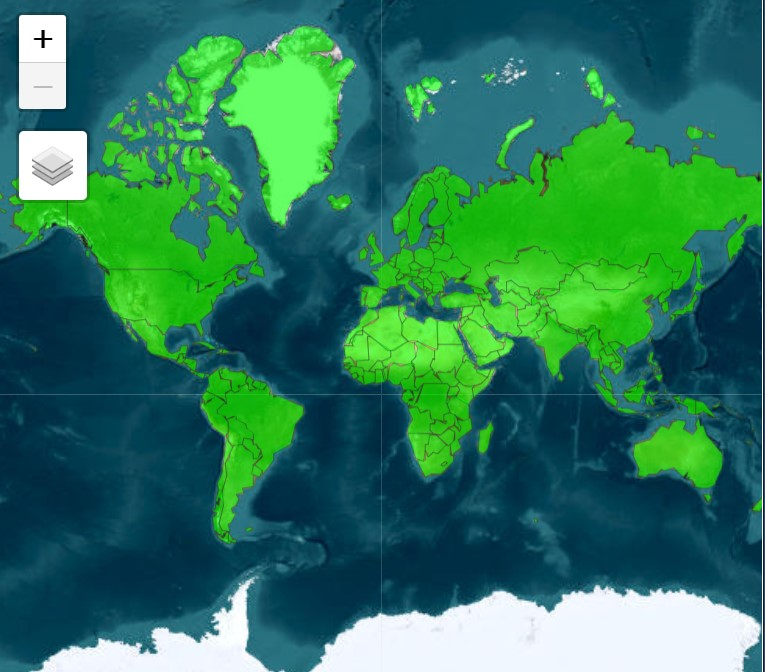
\includegraphics[width=1\linewidth]{E_IMAGENES/area_estudio.jpg}
            \begin{justify}
                \textit{Nota.} Se muestra un mapa satelital global, resaltando las zonas terrestres verdes, omitiendo océanos y la Antártida.
            \end{justify}                    
            \label{area_estudio}
        \end{figure}

        En la siguiente fase del estudio, se seleccionó estratégicamente Perú como área de la aplicación del autocompletado de bandas o canales que le faltan a las imágenes MSS para parecerse espectralmente a las TM. Esta elección se justifica por la variada topografía y diversidad de ecosistemas del país, que van desde la costa del Pacífico hasta las alturas de los Andes, ofreciendo un escenario desafiante y representativo para la superresolución satelital. Se identificaron múltiples puntos de muestreo distribuidos a lo largo del país, en los cuales se extrajeron segmentos de imágenes MSS para su transformación a la resolución de imágenes TM. 

        \begin{figure}[H] 
            \caption{\doublespacing \\ \textit{Mapa del área para la validación de los modelos.}} 
            \centering
            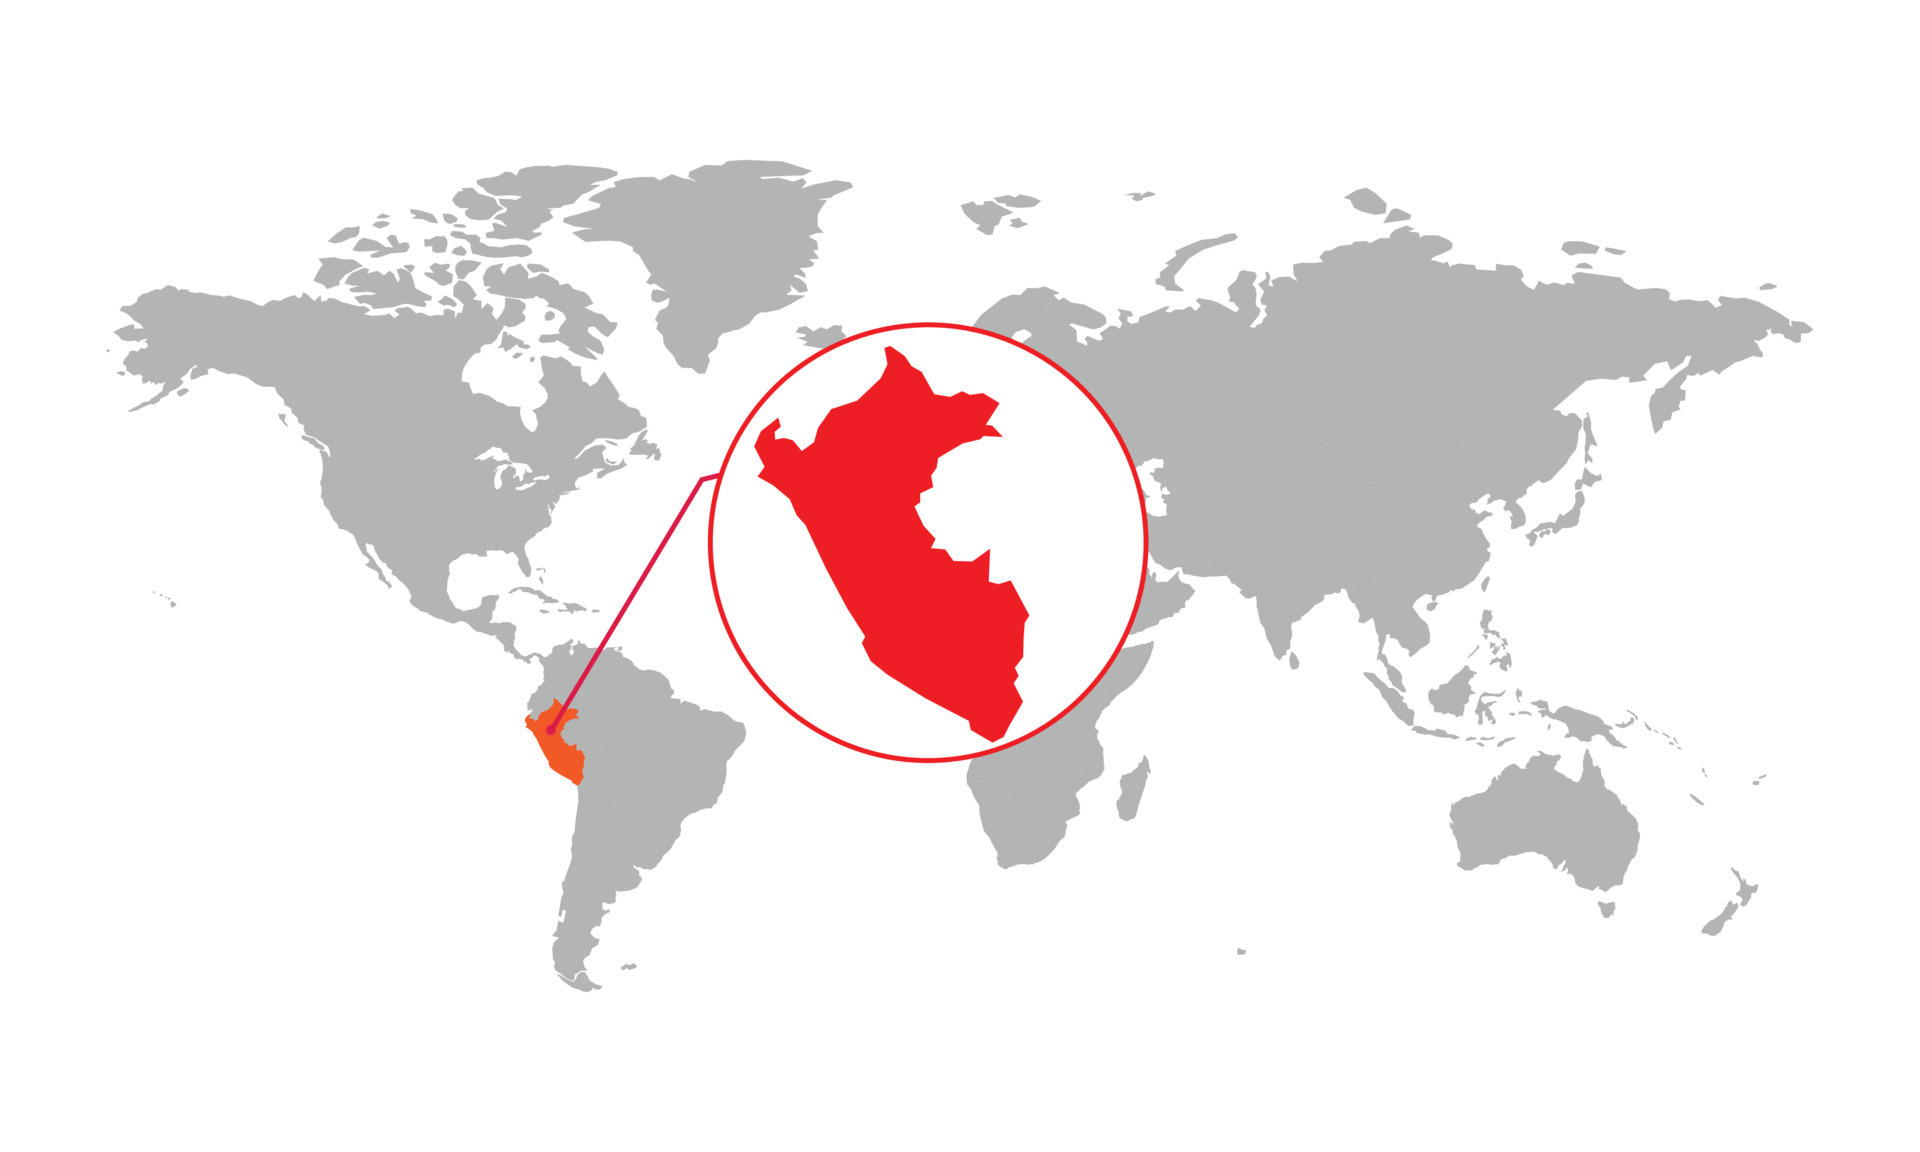
\includegraphics[width=0.8\linewidth]{2_CAPITULO4/IMG/mapa_peru.jpg}
            \begin{justify}
                \textit{Nota.} Se muestra un mapa de Perú, teniendo en cuenta toda su área, por su diversidad ecosistémica.
            \end{justify}                    
            \label{peru}
        \end{figure}

    \section{Diseño de investigación}
        En el marco del diseño de investigación de la tesis que aborda la armonización de imágenes Landsat MSS mediante inteligencia artificial, se adoptan criterios metodológicos que se alinean con los planteamientos de (Sampieri, 2018). Esta estructura metodológica se desglosa en las siguientes categorías:
        %\autocite{sampieri2018metodologia}
        \subsection{Tipo}
            La investigación se clasifica como aplicada, ya que tiene el objetivo de resolver problemas específicos relacionados con la armonización de imágenes satelitales, aplicando teorías y conocimientos de inteligencia artificial. Este tipo de investigación busca generar soluciones prácticas que puedan ser implementadas en el ámbito del monitoreo global y a largo plazo.

        \subsection{Nivel}
            Corresponde al nivel descriptivo, ya que se centra en describir las características y el comportamiento de un fenómeno o realidad específica, en este caso, la capacidad de la inteligencia artificial para mejorar la armonización de las imágenes Landsat MSS. A través de este nivel, se busca detallar las particularidades, diferencias o modalidades de un fenómeno sin ejercer control sobre las variables de estudio.

        \subsection{Enfoque}
            El enfoque de la investigación es cuantitativo, dado que se recopilan y analizan datos numéricos para evaluar la eficacia de los métodos de inteligencia artificial en la armonización de imágenes. Este enfoque permite una medición objetiva y estadística de los resultados, facilitando la comparación y el análisis de la efectividad de las técnicas empleadas.  

	    \subsection{Diseño}
            El diseño de esta investigación es no experimental, transeccional o transversal descriptivo. Esto significa que se observan fenómenos tal como se dan en su contexto natural para luego describirlos, sin manipular las variables de estudio. En este caso, se analiza la efectividad de la inteligencia artificial en la armonización de imágenes Landsat MSS, evaluando los datos existentes en un único momento, o en varios momentos bajo el mismo criterio, sin intervenir o modificar las condiciones bajo las cuales se obtuvieron dichas imágenes.

         
    \section{Población y muestra}
    
        \subsection{Población}
            La población de este estudio incluye imágenes capturadas por los sensores MSS y TM de los satélites Landsat 4 y 5, enfocándose en regiones continentales globales, excluyendo la Antártida y zonas oceánicas, entre 1982 y 1999. Estas imágenes, accesibles a través de las bases de datos de Landsat, ofrecen un registro histórico integral para la extracción de datos necesarios en esta investigación, permitiendo analizar las características y cambios en las regiones seleccionadas durante el periodo especificado.
            

        \subsection{Muestra}
            El enfoque de muestreo implementado es probabilístico, lo cual implica la selección aleatoria de unidades de muestreo para asegurar la independencia estadística y representatividad de las imágenes MSS y TM de Landsat en la muestra. Estas imágenes son elegidas basándose en criterios específicos, incluyendo un intervalo de tiempo de captura menor a 10 minutos entre ellas y una cobertura de nubosidad inferior al 15 \%, además de cumplir con requisitos de concordancia espacial. Siguiendo los lineamientos propuestos por \textcite{hernandez2014recoleccion} sobre recolección de datos, se ha establecido un tamaño de muestra de 5431 pares de imágenes. Esta cifra refleja adecuadamente la totalidad de la población estudiada, garantizando un análisis robusto y representativo de los datos.
            
    \section{Procedimiento, técnicas e instrumentos de recolección de información}

       \subsection{Obtención de datos de entrada}
            \subsubsection{Selección por localización}
                Para garantizar la eficacia y precisión de la investigación, se llevó a cabo una meticulosa selección de imágenes para el estudio. A continuación, se detalla el procedimiento de selección:
                
                \begin{enumerate}
                    \item Como punto de partida, se generaron puntos de manera aleatoria alrededor del mundo, resultando en un total inicial de 20 000 puntos. Estos puntos sirvieron como centroides para definir buffers cuadrados con dimensiones de 30 720 metros por lado.
                    
                    \begin{figure}[H] 
                        \caption{\doublespacing \\ \textit{Generación de 20 000 puntos aleatorios a nivel mundial.}} 
                        \centering
                        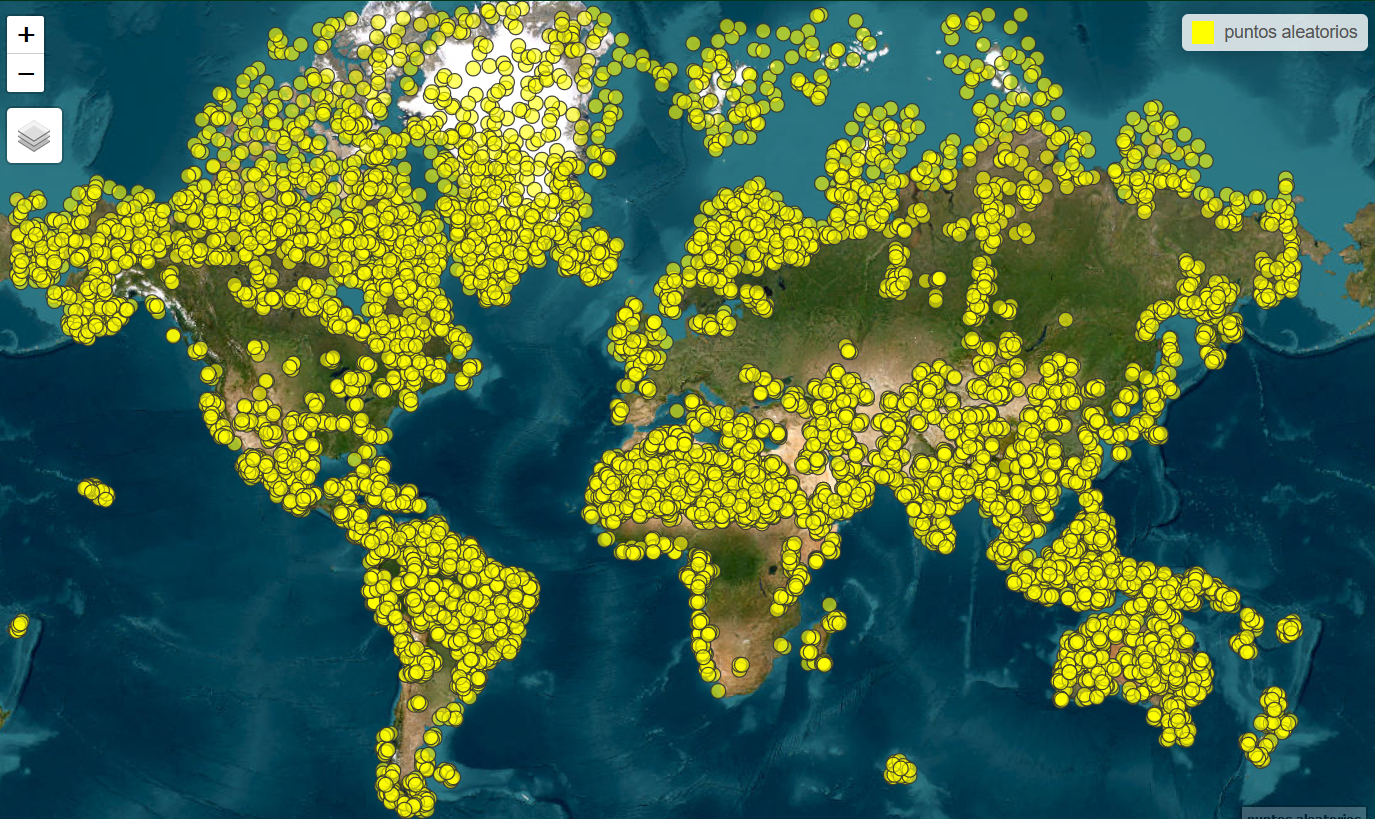
\includegraphics[width=0.9\linewidth]{2_CAPITULO0/IMG/1000points.png}
                        \begin{justify}
                            \textit{Nota.} Los puntos no excedieron los límites del WRS-2 (desde Landsat 4 hasta Landsat 9), que corresponden a las áreas o segmentos de captura de todas las imágenes Landsat, incluyendo los sensores más recientes.
                        \end{justify}                    
                        \label{1000points}
                    \end{figure}

        
                    \item Con los puntos geográficos establecidos, se procedió a seleccionar imágenes específicas. Se optó por imágenes MSS pertenecientes exclusivamente a las misiones Landsat 4 y 5, ya que coinciden con las imágenes obtenidas por el sensor TM de las mismas misiones durante el período de 1982 a 1999.
                
                    \item Una condición crucial en esta fase fue asegurar que el área definida por cada buffer estuviera íntegramente contenida dentro de al menos una imagen MSS y una imagen TM. Este criterio busca prevenir truncamientos o limitaciones en la amplitud de las imágenes.
                    
                    \item Se excluyeron ciertas áreas geográficas del proceso: específicamente, regiones de la Antártida y zonas mayormente oceánicas, para asegurar la relevancia y calidad del conjunto de datos final.
                    
                    \item Tras aplicar todos los criterios anteriores, de los 20 000 puntos iniciales, solo 19 546 satisfacían todas las condiciones y, por lo tanto, fueron retenidos para el estudio.
                \end{enumerate}
            \subsubsection{Selección por tiempo y calidad}
                Tras el filtro geográfico inicial, se procedió a una selección más detallada basada en criterios temporales y de calidad. A continuación se describe el procedimiento adoptado:
                
                \begin{enumerate}
                    \item De los 20 000 puntos iniciales, solo 19 546 cumplían con los criterios de localización. Para estos puntos seleccionados, se llevó a cabo una comparación temporal entre las imágenes de ambos sensores.
                
                    \item La condición impuesta fue que las imágenes de ambos sensores debían tener un diferencial temporal no superior a 10 minutos. Es decir, por cada punto, se retuvieron solo aquellos pares que hubieran sido capturadas en un intervalo de tiempo menor o igual a 10 minutos entre ellas.
                    
                    \item Es importante mencionar que este filtro temporal se aplicó considerando imágenes de los niveles Tier 1 y Tier 2 para ambos sensores. Debido a este riguroso criterio, no todos los puntos conservaron la misma cantidad de imágenes, y algunos incluso quedaron sin imágenes que cumplieran con este requisito.
                    
                    \item Posterior al filtro temporal, se implementó un filtro de calidad basado en la nubosidad. Se utilizó la banda de calidad (QA), específicamente de las imágenes del sensor TM, para evaluar la presencia de nubes o sombras. El criterio adoptado fue que las imágenes retenidas no debieran tener una cobertura de nubes o sombras que superara el 15\% del área del buffer generado por el punto dentro de la extensión de la imagen.
                    
                    \item Al concluir estos filtros, se obtuvo un conjunto final de imágenes (15 878 pares) filtradas que satisfacen tanto los criterios de diferencial temporal como los de calidad en relación con la nubosidad.
                \end{enumerate}
                
                Este enfoque garantizó un conjunto de datos con alta precisión temporal y calidad visual, minimizando las distorsiones o interferencias potenciales debido a la nubosidad.

                \begin{figure}[H] 
                    \caption{\doublespacing \\ \textit{Aplicación del algoritmo Fmask en imágenes TM para enmascarar nubes y reducir su interferencia en menos del 15\%.}} 
                    \centering
                    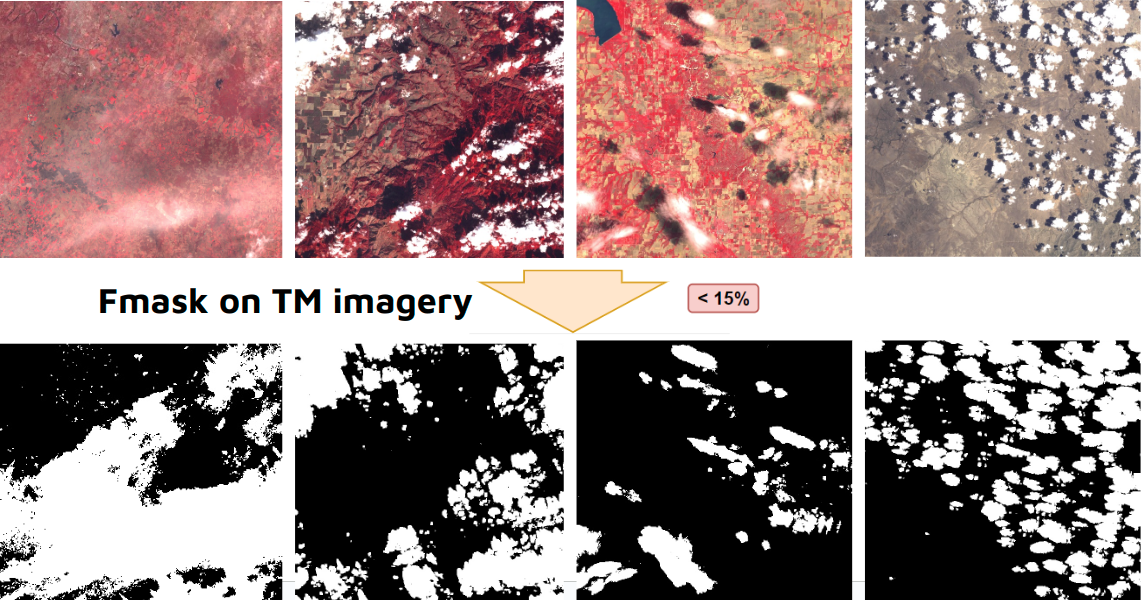
\includegraphics[width=1\linewidth]{2_CAPITULO4/IMG/fmask.png}
                    \begin{justify}
                        \textit{Nota.} El filtrado por nube es una etapa crítica en el procesamiento de imágenes satelitales, se utilizó el algoritmo Fmask para identificar y enmascarar nubes en imágenes de TM (Thematic Mapper), este proceso permite reducir la interferencia de nubes en menos del 15\%, mejorando la calidad de los datos utilizados para análisis posteriores.
                    \end{justify}                    
                    \label{fmask}
                \end{figure}
  
        \subsection{Corrección geométrica de las imágenes MSS}
            El propósito de este proceso es asegurar una alineación precisa entre las imágenes MSS y TM. A continuación, se detallan las etapas de la corrección geométrica:
            
            \subsubsection{Lectura y preprocesamiento de imágenes}
                Se cargan las imágenes, y son normalizadas para tener valores reales de reflectancia. Se seleccionan únicamente las bandas que coinciden entre las imágenes, garantizando su comparabilidad.
            
            \subsubsection{Extracción y coincidencia de características}
                Con la ayuda de modelos de aprendizaje profundo como LightGlue, se identifican puntos clave en ambas imágenes. Estos puntos son luego emparejados para determinar la desalineación entre las imágenes MSS y TM.
                
                \begin{figure}[H] 
                    \caption{\doublespacing \\ \textit{LightGlue: Emparejamiento de Características en Imágenes con Mecanismo Adaptativo.}} 
                    \centering
                    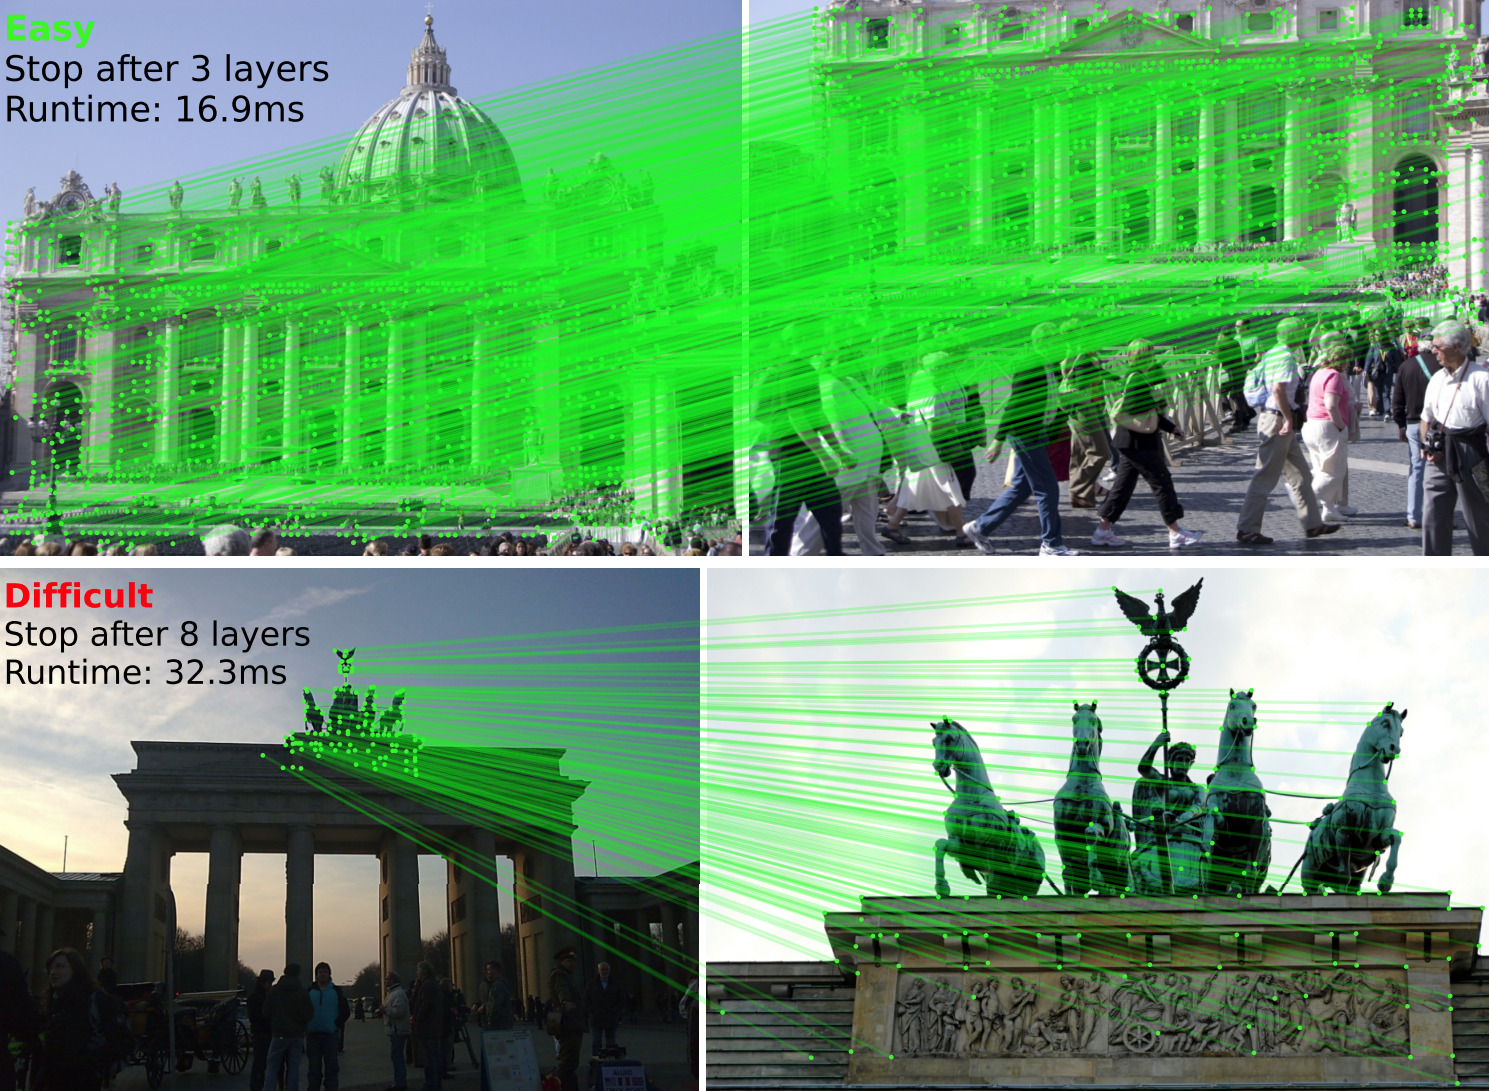
\includegraphics[width=1\linewidth]{2_CAPITULO0/IMG/cvg.png}
                    \begin{justify}
                        \textit{Nota.} La interfaz de 'LightGlue' exhibe dos ejemplos: uno 'fácil' con características emparejadas del Vaticano en 16.9ms y tres capas de procesamiento, y otro "difícil" de un monumento con estatuas, procesado en 32.3ms y ocho capas. Obtenido de \textcite{LightGlue2023}.
                    \end{justify}                    
                    \label{cvg}
                \end{figure}
                
            \subsubsection{Eliminacón de errores calidad y la usabilidad de las MSS}
                En las ímagenes MSS se mostraron errores de líneas saturadas y datos faltantes. Gracias a esta correción se eliminó estos errores, descartando los pares que presentaron estos problemas.

                \begin{figure}[H] 
                    \caption{\doublespacing \\ \textit{Imágenes MSS eliminados por errores del sensor.}} 
                    \centering
                    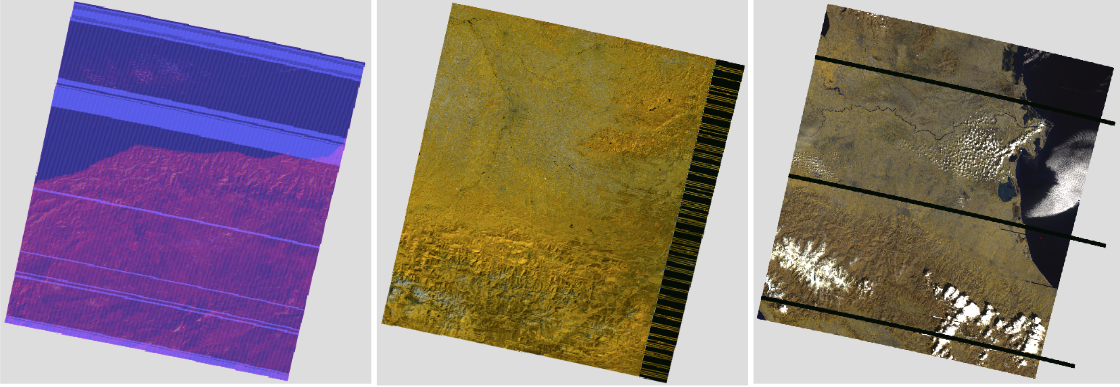
\includegraphics[width=1\linewidth]{2_CAPITULO4/IMG/mss_errores.png}
                    \begin{justify}
                        \textit{Nota.} Corrección geométrica aplicada a imágenes MSS, eliminando errores que afectan la coincidencia con imágenes TM.
                    \end{justify}                    
                    \label{errores_mss}
                \end{figure}

            \subsubsection{Determinación del desplazamiento espacial}
                Usando los puntos clave coincidentes, se estima el desplazamiento espacial entre las imágenes. Este desplazamiento señala cuánto y cómo se desalinean las imágenes en términos de píxeles.

                \begin{figure}[H] 
                    \caption{\doublespacing \\ \textit{Emparejamiento adaptativo de características con LightGlue: De alta resolución (HR) a baja resolución (LR).}} 
                    \centering
                    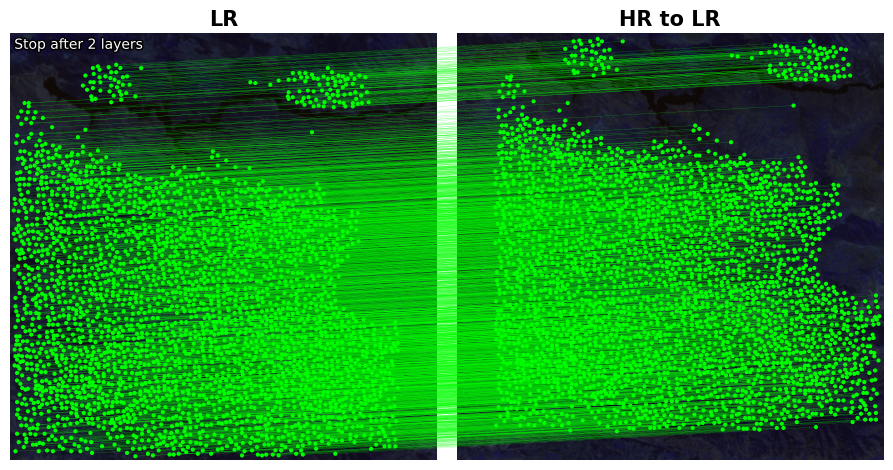
\includegraphics[width=1\linewidth]{2_CAPITULO0/IMG/hr_to_lr.png}
                    \begin{justify}
                        \textit{Nota.} Se observan superposiciones verdes de características detectadas, deteniéndose en ambas tras dos capas, evidenciando la eficacia de "LightGlue".
                    \end{justify}                    
                    \label{hr_to_lr}
                \end{figure}
                
            \subsubsection{Refinamiento subpíxel y convolución en 2D}
                Para refinar la corrección, se recurre a la transformada de Fourier. Esta técnica, mediante la función de correlación cruzada en el dominio de frecuencia, equivale a una convolución en 2D en el dominio espacial. La convolución en 2D es una operación que toma dos imágenes de entrada y produce una tercera imagen como salida, siendo una técnica fundamental en procesamiento de imágenes para filtrar y enfocar. Aquí, ayuda a identificar desplazamientos subpíxeles basados en el contenido de frecuencia de las imágenes.
                
                \begin{equation}
                    X(f) = \int_{-\infty}^{\infty} x(t) \cdot e^{-j2\pi ft} dt
                \end{equation}
            
                Donde \(X(f)\) es la transformada de Fourier de la señal \(x(t)\).
                
                
                Con base en el desplazamiento determinado y su refinamiento subpíxel, las imágenes MSS son alineadas geométricamente con las TM.
                
                Las imágenes MSS corregidas se presentan junto con las TM para confirmar visualmente la alineación. A través del proceso de corrección, se observa una mejora notable en la alineación, evidenciada por la reducción del desajuste visual entre las imágenes. Esta mejora se logra mediante correcciones tanto a nivel de píxel como subpíxel, lo que resulta en una superposición más precisa entre las imágenes MSS y TM.
                
                
                
            \subsubsection{Filtro final de los pares de imágenes}
                En complemento a las técnicas previamente descritas, se incorpora un criterio adicional para la exclusión de correspondencias erróneas entre las imágenes. Se establece un umbral de exclusión para desplazamientos que superen los 90 metros, equivalentes a 3 píxeles, con el objetivo de asegurar realismo y precisión en la alineación, descartando así anomalías significativas. Este enfoque resulta esencial debido a discrepancias previamente observadas entre las ubicaciones de las imágenes MSS y la realidad, utilizando como referencia las imágenes TM. Para optimizar el proceso, se implementa un filtro automatizado en lugar de una revisión visual individual.

                Posteriormente, se calcula el error cuadrático medio de colocación con los puntos restantes, un paso crítico para evaluar la precisión en la alineación de las imágenes MSS de baja resolución (LR) con las TM de alta resolución (HR). Se decide excluir del análisis cualquier par de imágenes cuyo error supere los 0.75 píxeles, con el fin de garantizar una alineación de alta precisión y minimizar desajustes residuales.
            
                Este rigor en la selección asegura la retención en el conjunto de datos únicamente de aquellas imágenes con una alineación casi perfecta, incrementando así la confiabilidad de los resultados. La combinación de este criterio con las correcciones a nivel de píxel y subpíxel conduce a una mejora notable en la alineación de las imágenes MSS y TM, reflejada en una reducción significativa del error RMSE.
            
                Finalmente, tras aplicar estos criterios de selección y refinamiento, se obtuvo un conjunto final de 5431 pares de imágenes. Estos pares seleccionados constituyen la base de datos con la que se entrenará el primer modelo de armonización de bandas, proporcionando una fundación sólida y precisa para el análisis y desarrollo del modelo.
        % \subsection{Aplicación de parámetros BRDF}
            %     Siguiendo el proceso de selección y filtrado de imágenes basado en criterios de diferencial temporal y calidad en relación con la nubosidad, se procedió con la aplicación de parámetros BRDF a las imágenes Landsat MSS y TM seleccionadas. Este paso fue fundamental para ajustar las imágenes a una base común de reflectancia, considerando las variaciones angulares y de iluminación inherentes a la captura de datos de satélite.
                
            %     \subsubsection{Selección y Preparación de Imágenes}
            %         Se seleccionaron imágenes pares de MSS y TM que correspondían en términos de ubicación y tiempo. La aplicación de parámetros BRDF a estas imágenes fue crucial para homogeneizar la reflectancia, permitiendo comparaciones precisas entre ellas.

            %     \subsubsection{Procesamiento con librecubo-brdf}
            %         Para la aplicación de correcciones BRDF, se utilizó el paquete librecubo-brdf, el cual implementa el método c-factor. Este método ajusta la reflectancia de las imágenes en función de su posición respecto al nadir y la iluminación solar, alineándolas con el concepto de Nadir BRDF Adjusted Reflectance (NBAR). Esta normalización es vital para una interpretación uniforme y precisa de los datos de reflectancia.

            %     \subsubsection{Homogeneización espectral}
            %         Con la aplicación de los parámetros BRDF, las imágenes pares quedaron normalizadas en términos de reflectancia. Este ajuste aseguró que las diferencias observadas en análisis posteriores reflejaran variaciones reales en las características de la superficie terrestre, y no artefactos debidos a la variabilidad en la captura de datos.


        \subsection{Preparación y organización de datos para deep learning}
            La fase de preparación y organización de datos es fundamental en el proceso de armonización de bandas entre las imágenes MSS de baja resolución (LR) y TM alta resolución (HR). Este proceso se estructura en varias etapas clave para garantizar la calidad y eficiencia del modelo de deep learning. Los procesos siguientes se establecen en el marco de la creación del Dataset y el DataLoader.

            \subsubsection{Conversión de formato de datos}
                Los datos originales en formato TIFF fueron transformados al formato SafeTensor, un cambio crucial para el almacenamiento y manejo eficiente de grandes volúmenes de datos. Esta conversión facilitó un acceso más rápido y una gestión más eficaz en los procesos de aprendizaje automático.

            \subsubsection{Estandarización y homogeneización}
                Se estandarizaron los datos para garantizar una estructura uniforme y coherente. La normalización de metadatos, el uso de esquemas JSON y la estructuración detallada de los datos aseguraron la integridad y la calidad de la información procesada.

            \subsubsection{Integración con Hugging Face}
                Los datos procesados y estandarizados se alojaron en la plataforma en la nube Hugging Face, proporcionando un acceso accesible y compartible. Esta integración facilitó la colaboración y el acceso a los datos para aplicaciones futuras en diversos proyectos.
            

                \paragraph{Publicación en Hugging Face}
                    Los datos en formato safetensor fueron subidos a la plataforma de Hugging Face, proporcionando un medio accesible y estandarizado para que investigadores y desarrolladores pudieran utilizarlos en futuros experimentos y validaciones.

                \paragraph{Catalogación efectiva}
                    El uso de ML-STAC fue esencial para catalogar y describir los conjuntos de datos de observación terrestre de manera unificada y optimizada. Esta metodología aseguró una gestión eficiente de los datos y facilitó su uso en aplicaciones de aprendizaje automático.

                \paragraph{Acceso y reproducibilidad}
                    La implementación de ML-STAC permitió el acceso a los datos bajo demanda y garantizó una reproducibilidad fiable de los experimentos y análisis realizados, abriendo la puerta a futuras investigaciones y validaciones independientes.

            \subsubsection{Segmentación y distribución de datos}
                Con un total de 5431 pares de imágenes MSS y TM, se realiza una cuidadosa segmentación del conjunto. Esta segmentación resulta en una distribución donde aproximadamente el 81\% de los datos se asignan para entrenamiento, mientras que el 9\% se destina a la validación y otro 10\% para pruebas. Esta división equilibrada es crucial para evaluar adecuadamente la capacidad del modelo en diferentes conjuntos de datos.
            
            \subsubsection{Procesamiento y alineación de imágenes} 
                Cada par de imágenes pasa por un proceso de procesamiento y alineación. Se realiza una cuidadosa eliminación de píxeles de borde y se aplica un recorte aleatorio para generar muestras de 256x256 píxeles en las imágenes MSS. Para las imágenes TM, se utiliza la técnica de interpolación bilineal con antialiasing para ajustar su resolución, mejorando la calidad visual y reduciendo artefactos.
            
            \subsubsection{Normalización y preparación de datos} 
                Las imágenes procesadas son normalizadas para asegurar la consistencia en la escala de valores de píxeles. Esta normalización es esencial para la eficiencia del aprendizaje, asegurando que tanto las imágenes MSS como las TM contribuyan de manera equitativa al entrenamiento del modelo. 
            
            \subsubsection{Optimización y manejo eficiente de datos} 
                Los dataloaders se configuran para optimizar la carga y manejo de los datos durante el entrenamiento y la validación. Se establecen parámetros específicos como el tamaño del lote y el número de hilos de procesamiento, buscando una mayor eficiencia y un uso óptimo de los recursos computacionales.
            
                \begin{figure}[H] 
                    \caption{\doublespacing \\ \textit{Flujo del proceso de preparación y organización de datos.}} 
                    \centering
                    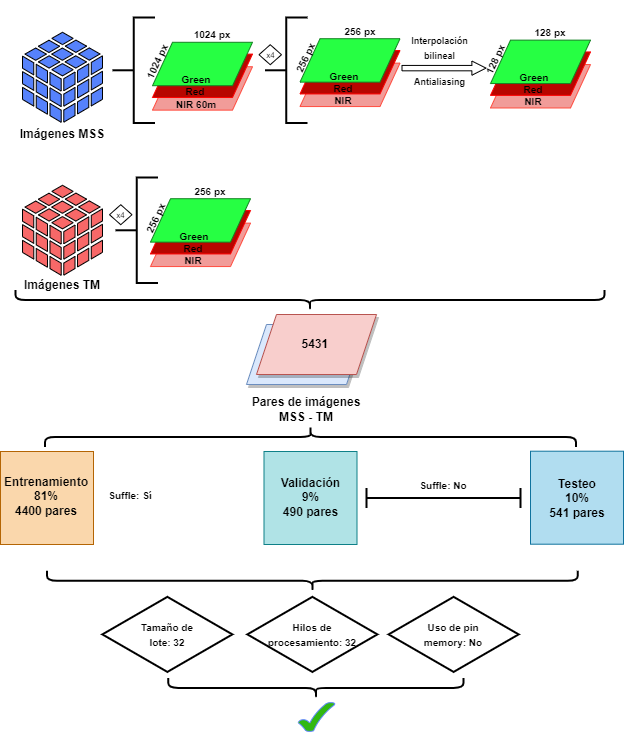
\includegraphics[width=1\linewidth]{2_CAPITULO4/IMG/dataloader.png}
                    \begin{justify}
                        \textit{Nota.} El gráfico detalla el flujo de datos en la preparación de imágenes satelitales MSS y TM, su segmentación en lotes y la configuración eficiente de dataloaders para el modelo.
                    \end{justify}                    
                    \label{dataloader}
                \end{figure}

                Este proceso no solo facilita el manejo eficiente de los datos, sino que también asegura que cada par de imágenes MSS y TM sea procesado y presentado al modelo de manera óptima, mejorando la precisión y efectividad del entrenamiento para la armonización de bandas.



        \subsection{Desarrollo del modelo MSS2TM}


        
            \subsubsection{Configuración del entorno de trabajo}
                Se estableció un entorno de trabajo en Python mediante la creación de un entorno virtual utilizando herramientas como entornos de conda. Esto permitió una separación clara y la gestión de dependencias específicas del proyecto. Se instaló PyTorch, seleccionando una versión que correspondiera a la compatibilidad con CUDA del sistema utilizado, para facilitar el entrenamiento acelerado por GPU.
            
                Además, se implementaron herramientas de registro y monitoreo para seguir el progreso del entrenamiento y se estableció un sistema de control de versiones para el código y los datos. La automatización y orquestación del flujo de trabajo, junto con la validación del código mediante pruebas unitarias y de integración, formaron parte esencial de este proceso. Todas las dependencias se documentaron en un archivo requirements.txt para facilitar la configuración reproducible del entorno.


            \subsubsection{Elección de arquitecturas para el generador y discriminador en GANs}
                En la fase de desarrollo del modelo se escogió con detenimiento la arquitectura para cada componente de la Red Neuronal Generativa Adversaria (GAN), fundamental para la consecución de nuestros objetivos. El generador, implementado como un Transformer Visual, conocido comúnmente por su acrónimo en inglés VIT (Vision Transformer), fue diseñado para procesar y transformar imágenes de múltiples espectros (MSS) en imágenes de alta resolución (HR) o TM. Esta elección se basó en la capacidad de los Transformers Visuales para manejar secuencias de datos, lo que resulta ideal para comprender y generar representaciones complejas de imágenes. Por otro lado, para el discriminador, se optó por una arquitectura de Perceptrón Multicapa (MLP), que debido a su simplicidad y eficacia en tareas de clasificación, resultó ser la más adecuada para evaluar la autenticidad de las imágenes generadas por el VIT, diferenciando entre las reales y las producidas artificialmente. 
            
         
                \begin{figure}[H] 
                    \caption{\doublespacing \\ \textit{Arquitectura de Super-Resolución para armonización de imágenes Landsat MSS y TM utilizando SWINIR.}} 
                    \centering
                    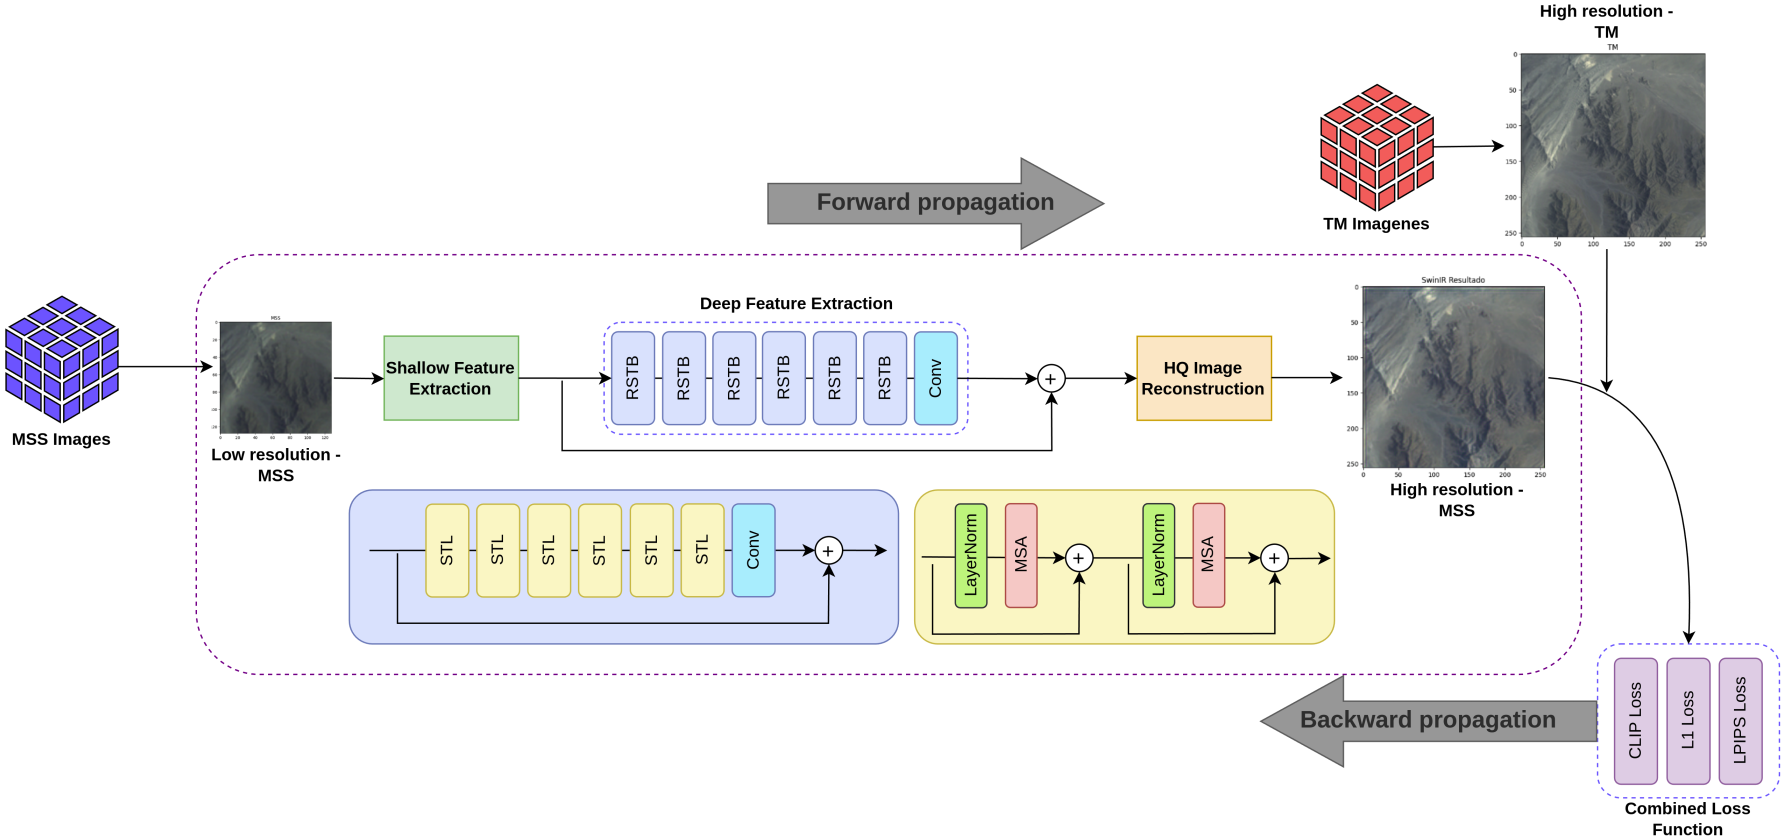
\includegraphics[width=1\linewidth]{2_CAPITULO4/IMG/SWINIR.png}
                    \begin{justify}
                        \textit{Nota.} El diagrama muestra el proceso de extracción y reconstrucción de características para convertir imágenes de baja resolución MSS en alta resolución utilizando SWINIR, integrando módulos RSTB y STL para mejorar la calidad de las imágenes resultantes.
                    \end{justify}                    
                    \label{generador}
                \end{figure}
    

                \begin{figure}[H] 
                    \caption{\doublespacing \\ \textit{Flujo del discriminador MLP.}} 
                    \centering
                    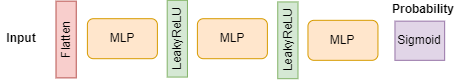
\includegraphics[width=0.6\linewidth]{2_CAPITULO5/IMG/mlp_discriminator.png}
                    \begin{justify}
                        \textit{Nota.} Se muestra un flujo del discriminador MLP inicia con entrada de imagen, pasa por capas MLP y Leaky ReLU, culmina con probabilidad sigmoide.
                    \end{justify}                    
                    \label{discriminador}
                \end{figure}

            \subsubsection{Definición de parámetros y funciones de pérdida}
                Se definieron las funciones de pérdida para entrenar el modelo. El L1 Loss se utilizó para minimizar la diferencia absoluta píxel por píxel entre las imágenes generadas por el modelo (\(TM_{hat}\)) y las imágenes objetivo (TM), con el fin de asegurar una alta fidelidad visual. Además, se implementó una función de pérdida adicional para el discriminador, donde se estimó la probabilidad de que una imagen sea real o falsa (L2), promoviendo la generación de imágenes que el discriminador no pudiera distinguir de las reales.

            \subsubsection{Proceso de entrenamiento}
                En la fase de entrenamiento, se ajustaron los parámetros de los modelos generador y discriminador de manera iterativa. Se comenzó con una tasa de aprendizaje adaptativa y un coeficiente \( \alpha \) inicialmente establecido en 0.5 para equilibrar las funciones de pérdida L1 y L2. Tras experimentación empírica, se estableció que un \( \alpha \) de 0.01 proporcionaba un equilibrio más efectivo, reduciendo las distorsiones en las imágenes generadas y mejorando la estabilidad del entrenamiento. La optimización se llevó a cabo utilizando el algoritmo Adam, y se incorporó la técnica de dropout para prevenir el sobreajuste. A lo largo del proceso, la pérdida observada disminuyó de manera sostenida, lo que indicó una mejora continua en la precisión del modelo. Además, se emplearon técnicas de aumento de datos y selección aleatoria de lotes para fortalecer la robustez del entrenamiento.

                Durante esta fase, también se enfatizó la importancia de una inicialización adecuada y un registro detallado del proceso. Se utilizó PyTorch por su eficiencia y flexibilidad, configurando aspectos fundamentales como la semilla aleatoria y el dispositivo de cálculo para asegurar un entrenamiento estable y reproducible. Herramientas de registro como Weights and Biases (wandb) permitieron monitorear en tiempo real métricas clave como la pérdida y la precisión, facilitando un seguimiento detallado del entrenamiento.

                La carga de datos se optimizó mediante la biblioteca ML-STAC, lo que garantizó una gestión eficiente de los grandes conjuntos de datos de imágenes satelitales. Este enfoque uniformó la carga de datos y mejoró la integración de los mismos en el entrenamiento.

                El cálculo de métricas específicas como la pérdida L1, la pérdida perceptual y la pérdida GAN proporcionó información valiosa sobre el rendimiento del modelo, ayudando en la afinación y el ajuste de hiperparámetros. La implementación de un sistema de checkpointing aseguró la recuperación del entrenamiento en caso de interrupciones, facilitando la experimentación con diferentes configuraciones y el almacenamiento periódico de los estados del modelo, la configuración del optimizador y otros hiperparámetros.

            \subsubsection{Ajuste y optimización}
                El proceso de ajuste fino del modelo, que comprende tanto el generador, implementado con la arquitectura VIT, como el discriminador, basado en un MLP, fue crucial para lograr resultados satisfactorios. Durante esta etapa, se experimentó con variaciones en los hiperparámetros y se aplicó la validación cruzada para asegurar la generalización del modelo. Para el discriminador, se desarrolló una estrategia de entrenamiento que moderaba la actualización de sus parámetros, buscando mantener el equilibrio de Nash y evitar el colapso del modelo. Este cuidadoso ajuste se extendió al generador, donde se aplicaron técnicas como la corrección de máscaras basada en cuantiles y operaciones de división o sustracción, permitiendo refinar la representación de las imágenes generadas. Se emplearon tanto el \(L1\) Loss, para minimizar la diferencia absoluta píxel por píxel entre las imágenes generadas y las de referencia, asegurando así una alta fidelidad visual, como el \(L2\) Loss, para evaluar la capacidad del generador de producir imágenes que el discriminador considere reales. La combinación de estas estrategias resultó en una notable mejora en la precisión, fidelidad y realismo de las imágenes generadas, validando la eficacia de las arquitecturas y metodologías de entrenamiento empleadas.

            
                \subsubsection{Configuración de las funciones de pérdida}
                    La eficacia de un modelo de superresolución como MSS2TM depende en gran medida de las funciones de pérdida utilizadas durante el entrenamiento. Estas funciones de pérdida son cruciales para guiar el proceso de aprendizaje del modelo hacia la generación de imágenes que no solo son visualmente atractivas, sino que también son fieles a las características reales de las imágenes de alta resolución. Para el modelo MSS2TM, se adoptó un enfoque multiobjetivo en la selección y configuración de las funciones de pérdida, basándose en la naturaleza de las imágenes MSS y TM.
                
                    \paragraph{CLIP Loss}
                        La función de pérdida CLIP (Contrastive Language-Image Pretraining) Loss se emplea para asegurar que las imágenes generadas sean coherentes con las características contextuales y semánticas aprendidas a partir de grandes conjuntos de datos de imágenes y texto. CLIP Loss utiliza un modelo preentrenado que compara las imágenes generadas con descripciones textuales, asegurando que las imágenes producidas no solo sean visualmente similares, sino que también mantengan una coherencia semántica con las descripciones esperadas.

                    \paragraph{L1 Loss}
                        El L1 Loss, también conocido como L1-norm loss o Mean Absolute Error (MAE), mide la diferencia absoluta entre los valores de los píxeles de la imagen generada y la imagen de referencia. Esta función de pérdida es esencial para asegurar que las imágenes generadas sean lo más similares posible a las imágenes de alta resolución en términos de detalles y texturas finas.

                    \paragraph{LPIPS Loss}
                        La función de pérdida LPIPS (Learned Perceptual Image Patch Similarity) se utilizó para evaluar la similitud perceptual entre las imágenes generadas y las de alta resolución. LPIPS aprovecha un modelo preentrenado para comparar las características visuales y contextuales de las imágenes. Esta función de pérdida es particularmente efectiva para asegurar que las imágenes superresueltas no solo coincidan en términos de píxeles, sino que también capturen con precisión los elementos y patrones semánticos presentes en las imágenes TM de alta resolución.

                    \begin{figure}[H] 
                        \caption{\doublespacing \\ \textit{Flujo  de la arquitectura GAN - MSS2TM para la armonización espectral y espacial.}} 
                        \centering
                        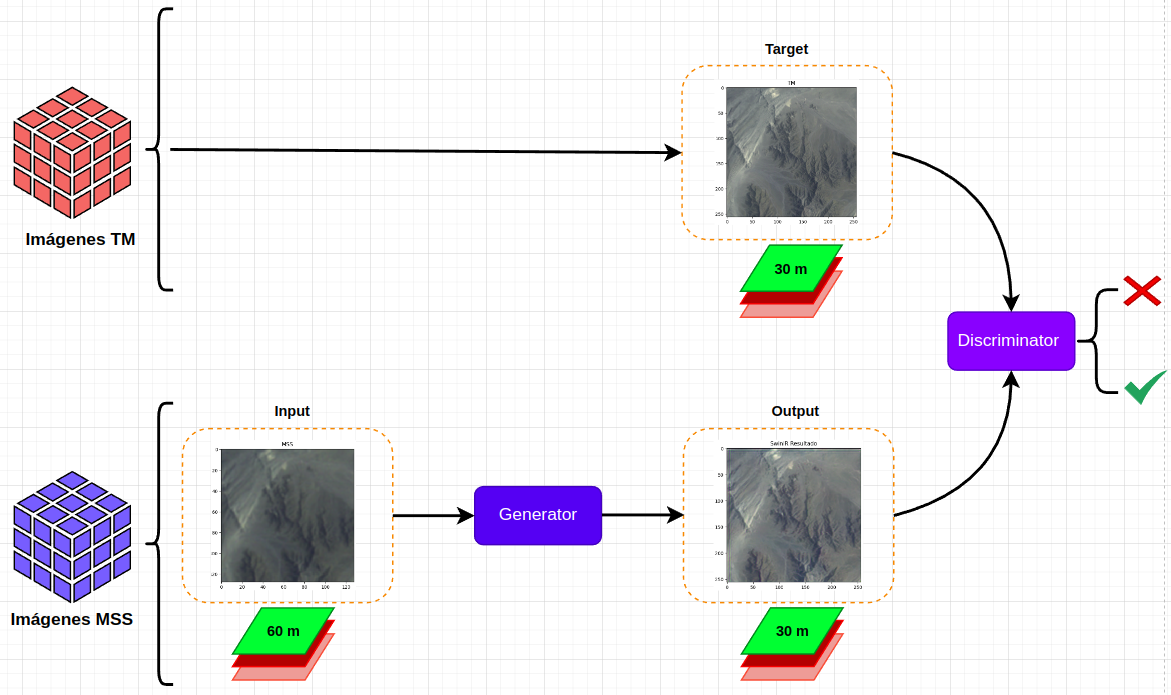
\includegraphics[width=1\linewidth]{2_CAPITULO4/IMG/GAN.png}
                        \begin{justify}
                            \textit{Nota.} El diagrama ilustra el flujo de trabajo de una arquitectura GAN para transformar imágenes MSS de 60m a una resolución de 30m, evaluadas por un discriminador para mejorar la armonización espectral y espacial​.
                        \end{justify}                    
                        \label{gan}
                    \end{figure}

        \subsection{Generación de bandas virtuales en imágenes MSS}
            Una vez que las imágenes MSS se alinean espectral y espacialmente con las TM gracias al modelo MSS2TM, el siguiente paso es generar bandas sintéticas o virtuales para las MSS que existen en las TM pero no en las MSS. 
            
            \subsubsection{Adquisición y procesamiento inicial de datos}
                Se comenzó con reconocer el sistema multiespectral MSS, que contenían bandas espectrales en el rango del infrarrojo cercano (NIR), rojo y verde, todas con una resolución de 30 metros.

            \subsubsection{Entrenamiento del perceptrón multicapa (MLP)}
                El diseño y entrenamiento de un MLP constituyó el núcleo del enfoque adoptado para predecir las bandas espectrales faltantes en las imágenes MSS. La red neuronal profunda se estructuró mediante la inclusión de capas lineales y una arquitectura que promovió el aprendizaje de patrones complejos por medio de activaciones no lineales y la regulación de conexiones entre neuronas. El propósito fue refinar los parámetros del modelo de manera que este pudiera replicar con exactitud las bandas adicionales necesarias, simulando efectivamente una imagen TM completa.

                La implementación del modelo MLP se realizó extendiendo la clase Module de PyTorch, integrando tres capas lineales (nn.Linear) intercaladas con funciones de activación no lineales (nn.ReLU) y una capa de abandono (nn.Dropout) para la regularización. La configuración de la red permitió la transformación de la entrada a un espacio de características ocultas, seguido por el procesamiento intermedio de estas características, y finalmente, su conversión al espacio de salida deseado mediante la última capa lineal. La inclusión de la función de activación ReLU facilitó el aprendizaje de relaciones complejas entre las entradas y las salidas, mientras que la capa de abandono contribuyó a la prevención del sobreajuste mediante el descarte aleatorio de algunas características durante el entrenamiento.
                
                La lógica de procesamiento de datos se definió en la función forward, asegurando el paso secuencial de los datos a través de las capas lineales, la activación ReLU y el abandono, antes de emitir la salida final.
                
                El entrenamiento del modelo se organizó a través de la función \texttt{run\_deep\_prior}, que inició con la preparación de los datos de entrada y salida en un formato adecuado. Posteriormente, se instanció el modelo MLP, configurando el optimizador Adam y la función de pérdida L1, esenciales para el proceso de aprendizaje.

            \subsubsection{Proceso de entrenamiento y ajuste fino}
                El modelo se sometió a un régimen de entrenamiento iterativo y exhaustivo, durante el cual se realizaron actualizaciones graduales y precisas en la configuración interna de la red. Se emplearon lotes de datos pequeños para optimizar los recursos computacionales y mejorar la capacidad del modelo para generalizar a partir de los datos proporcionados. La estrategia de entrenamiento estuvo guiada por un enfoque de minimización de errores, donde se buscaba reducir la diferencia entre las bandas espectrales conocidas y las predicciones del modelo.

                \paragraph{Histograma matching}
                    El \textit{histograma matching} se utiliza para normalizar los valores de reflectancia entre diferentes imágenes. Este proceso implica corregir los histogramas de las imágenes para que tengan una distribución similar, lo cual es crucial para mantener la coherencia en las bandas generadas.

                \paragraph{Normalización de valores de reflectancia}
                    El modelo también intenta normalizar los valores de reflectancia. Este proceso es complicado debido a que las mismas bandas de diferentes imágenes pueden tener distintos valores de reflectancia. La normalización correcta es esencial para obtener resultados precisos en la generación de imágenes de mayor resolución.

                \paragraph{Modelos con diferentes parámetros}
                    La comparación entre modelos con distintos números de parámetros (por ejemplo, 68 vs. 128 parámetros) es importante para evaluar el impacto en el rendimiento y la precisión de la superresolución. Además, fue crucial encontrar el número adecuado de iteraciones (por ejemplo, 2000 pasos) para entrenar el modelo, lo cual puede variar debido a la aleatoriedad en el entrenamiento.

                \paragraph{Early stopping}
                    Implementar \textit{early stopping} fue una estrategia eficaz para detener el entrenamiento del modelo una vez que alcanza una meseta en su rendimiento. Esto evitó el sobreentrenamiento y mejora la eficiencia del modelo, permitiendo un uso óptimo de los recursos computacionales.

                \paragraph{Mantener la firma espectral}
                    La preservación de la forma de la firma espectral fue crucial para asegurar la precisión en la generación de bandas. No solo fue importante mantener los valores de intensidad, sino también la forma de la firma espectral. Esto pudo requerir ajustar los parámetros del modelo, aumentando su complejidad para mantener la integridad espectral.


            \begin{figure}[H] 
                \caption{\doublespacing \\ \textit{Modelo de armonización para imágenes Landsat MSS.}} 
                \centering
                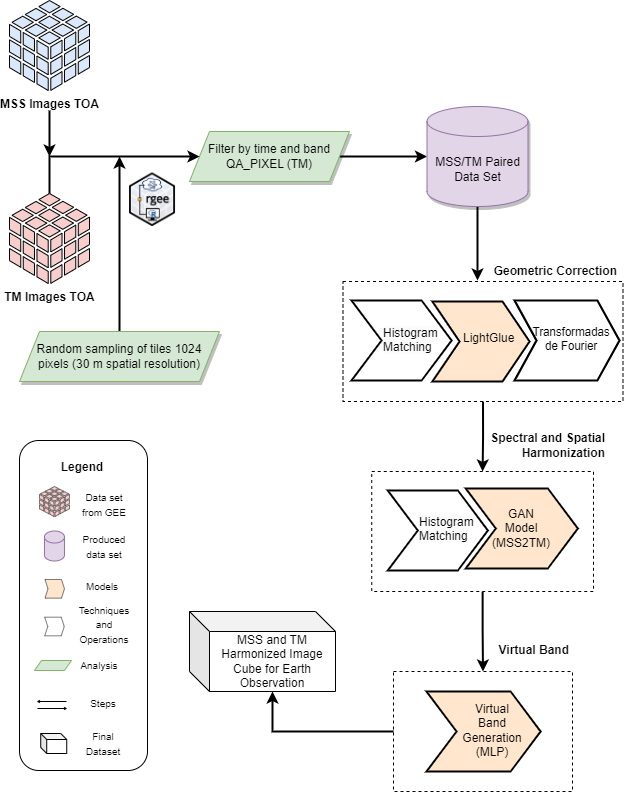
\includegraphics[width=0.95\linewidth]{2_CAPITULO5/IMG/modelo.png}
                \begin{justify}
                    \textit{Nota.} El esquema presenta una metodología de armonización de imágenes de sensores MSS y TM: comienza con imágenes TOA, sigue con correcciones geométricas y transformadas de Fourier via LightGlue, continúa con armonización espectral y espacial mediante una arquitectura GAN y culmina con un cubo de imagen armonizado para la creación de bandas virtuales.
                \end{justify}                    
                \label{modelo2}
            \end{figure}

    \section{Análisis estadístico}

        En la fase de preparación para la validación de los modelos desarrollados, se diseñó un enfoque de análisis estadístico detallado. Este diseño metodológico fue crucial para asegurar que, una vez aplicados, los modelos pudieran demostrar un ajuste adecuado a los datos de entrenamiento y una generalización efectiva a nuevos conjuntos de datos.
            
        \subsection{Validación cuantitativa}
            
            Se emplearon las siguientes métricas para evaluar el desempeño del modelo:
            
            \subsubsection{Error Absoluto Medio (MAE)} 
                Esta métrica midió la diferencia media absoluta entre los valores predichos por el modelo y los valores reales. Fue útil para entender el error promedio por píxel en las imágenes generadas.
                
            \subsubsection{Raíz del Error Cuadrático Medio (RMSE)} 
                Similar al MAE, pero penalizó más los errores grandes, ofreciendo una visión más estricta de la precisión del modelo.
                
            \subsubsection{Coeficiente de Correlación de Pearson (R)} 
                Midió la relación lineal entre los valores predichos y los valores reales, proporcionando una medida de cuán bien las predicciones siguieron las tendencias reales.
            
        \subsection{Evaluación de métricas de rendimiento}
            
            Para asegurar que las imágenes generadas no solo coincidieran en términos de píxeles, sino que también capturaran con precisión los elementos y patrones semánticos presentes en las imágenes TM de alta resolución, se utilizaron las siguientes funciones de pérdida:
            
            \subsubsection{CLIP Loss} 
                Se empleó para asegurar que las imágenes generadas fueran coherentes con las características contextuales y semánticas aprendidas a partir de grandes conjuntos de datos de imágenes y texto. Utilizó un modelo preentrenado que comparaba las imágenes generadas con descripciones textuales.
                
            \subsubsection{L1 Loss} 
                También conocido como Mean Absolute Error (MAE), midió la diferencia absoluta entre los valores de los píxeles de la imagen generada y la imagen de referencia. Fue esencial para asegurar que las imágenes generadas fueran lo más similares posible a las imágenes de alta resolución en términos de detalles y texturas finas.
                
            \subsubsection{LPIPS (Learned Perceptual Image Patch Similarity) Loss} 
                Evaluó la similitud perceptual entre las imágenes generadas y las de alta resolución. Aprovechó un modelo preentrenado para comparar las características visuales y contextuales de las imágenes, asegurando que las imágenes superresueltas capturaran con precisión los elementos y patrones semánticos presentes en las imágenes TM de alta resolución.
                
	% \Chapter{}

\chapter{RESULTADOS}

    \section{Evaluación de la armonización de imágenes MSS y TM}
        \subsection{Corrección geométrica y alineación espacial}
            La aplicación de técnicas avanzadas de corrección geométrica y alineación espacial a las imágenes MSS resultó en una mejora significativa en la precisión de su superposición con las imágenes TM. Utilizando el método LightGlue para el emparejamiento de características, se logró una reducción notable en el error de colocación, pasando de un RMSE inicial de 52.6523 a un RMSE de 0.987. Este resultado subraya la efectividad de las correcciones a nivel de píxel y subpíxel en la alineación de las imágenes, permitiendo una base sólida para la posterior armonización espectral.

            \begin{figure}[H] 
                \caption{\doublespacing \\ \textit{Comparativa de alineación: imágenes MSS, TM y MSS corregida.}} 
                \centering
                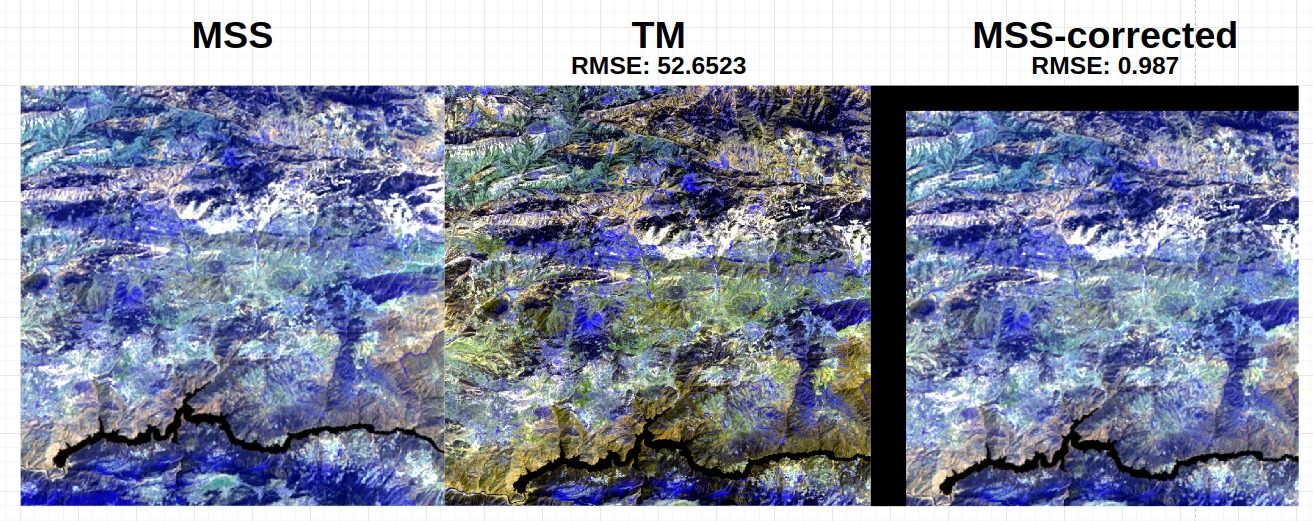
\includegraphics[width=1\linewidth]{2_CAPITULO0/IMG/tm_mss_rmse.png}
                \begin{justify}
                    \textit{Nota.} El contraste entre la imagen MSS original y la corregida resalta con una reducción significativa del error RMSE, evidenciando la eficacia de las correcciones a nivel de píxel y subpíxel para lograr una alineación casi perfecta.
                \end{justify}                    
                \label{tm_mss_rmse}
            \end{figure}

        \subsection{Calidad de la armonización espectral y espacial}
            La implementación del modelo SWINIR - MSS2TM GAN mostró una capacidad excepcional para armonizar las bandas espectrales de las imágenes MSS con las correspondientes imágenes TM. 

            \begin{figure}[H] 
                \caption{\doublespacing \\ \textit{Generación de bandas NIR-R-G armonizadas de MSS hacia TM.}} 
                \centering
                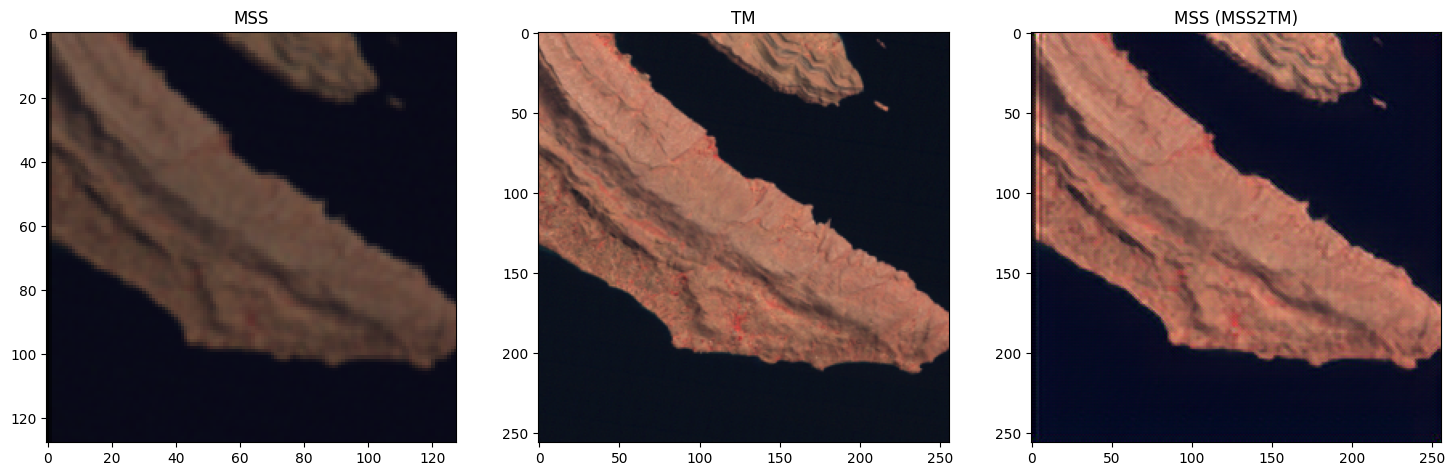
\includegraphics[width=1\linewidth]{2_CAPITULO5/IMG/espectral.png}
                \begin{justify}
                    \textit{Nota.} Comparación entre imágenes MSS, TM y MSS corregida usando el modelo SWINIR - MSS2TM. La imagen MSS original se muestra a la izquierda, la imagen TM original está en el centro, y la imagen MSS corregida se encuentra a la derecha, destacando la mejora en la armonización espectral.
                \end{justify}                    
                \label{armonizacion}
            \end{figure}
            
            \begin{figure}[H] 
                \caption{\doublespacing \\ \textit{Comparación de imágenes MSS antes y después de la mejora en resolución.}} 
                \centering
                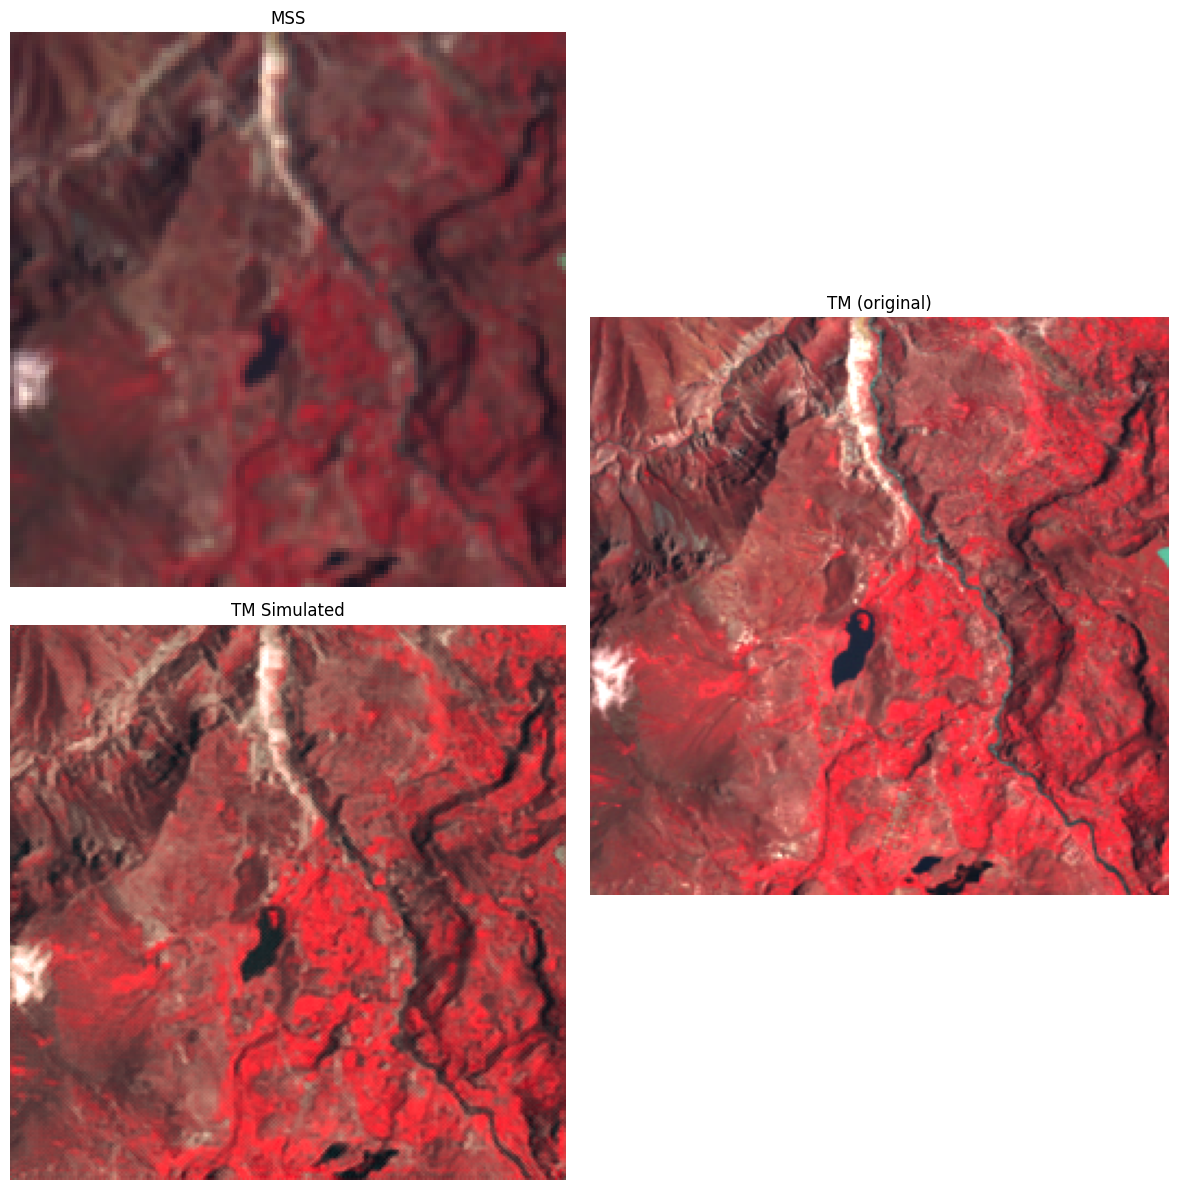
\includegraphics[width=0.8\linewidth]{2_CAPITULO5/IMG/espectral2.png}
                \begin{justify}
                    \textit{Nota.} Comparación de la resolución de imágenes MSS y TM. La imagen MSS original se muestra en la parte superior izquierda, la imagen TM simulada está en la parte inferior izquierda, y la imagen TM original se presenta a la derecha, demostrando la mejora en la resolución de la imagen MSS.
                \end{justify}                    
                \label{armonizacion2}
            \end{figure}
            


        \subsection{Generación de bandas virtuales}
            La creación de bandas virtuales para complementar las imágenes MSS con bandas no originalmente presentes demostró ser altamente efectiva. El modelo de Perceptrón Multicapa (MLP) empleado para predecir estas bandas adicionales alcanzó una alta precisión de predicción, reflejada en un bajo error medio absoluto (MAE). Esta técnica permite mejorar significativamente la calidad de las imágenes MSS, haciéndolas comparables a las imágenes TM en términos de resolución espectral.

            

            \begin{figure}[H] 
                \caption{\doublespacing \\ \textit{Comparación de imágenes Landsat MSS y TM.}} 
                \centering
                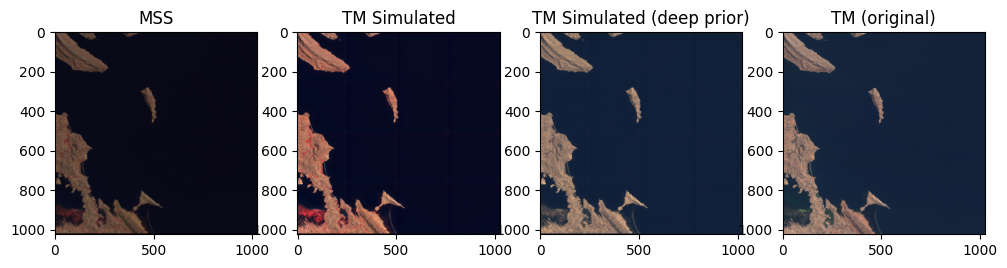
\includegraphics[width=1\linewidth]{2_CAPITULO5/IMG/bandas.png}
                \begin{justify}
                    \textit{Nota.} Visualización del avance en generación de bandas virtuales MSS, mostrando la eficacia del modelo MLP en la precisión espectral frente a imágenes TM originales.
                \end{justify}                    
                \label{bandas}
            \end{figure}

            \begin{figure}[H] 
                \caption{\doublespacing \\ \textit{Comparación de alineación y generación de bandas virtuales.}} 
                \centering
                \includegraphics[width=1\linewidth]{2_CAPITULO5/IMG/comparasion.png}
                \begin{justify}
                    \textit{Nota.} Comparativa de imágenes MSS original, TM simulada con 3 bandas, TM simulada con 7 bandas y TM original, mostrando mejoras en la precisión espectral con modelos avanzados como SWINIR y MLP.
                \end{justify}                    
                \label{bandas2}
            \end{figure}

            La mejora en la resolución es evidente al comparar la imagen MSS original con la imagen TM simulada. Esta mejora permite una mejor interpretación y análisis de los datos históricos de Landsat MSS.

        \subsection{Evaluación de la armonización de imágenes}

            \subsubsection{Índices espectrales} 

                Para evaluar la efectividad de la armonización de imágenes MSS y TM, se calcularon varios índices espectrales tanto para las imágenes originales como para las imágenes simuladas. Los índices utilizados incluyen el Índice de Vegetación de Diferencia Normalizada (NDVI), el Índice de Diferencia Normalizada de Agua (NDWI) y el Índice de Diferencia Normalizada de Nieve (NDSI).

                \paragraph{Índice de vegetación de diferencia normalizada (NDVI)}

                    El NDVI es una métrica importante para el análisis de la vegetación. Se calcula usando las bandas roja (Red) y del infrarrojo cercano (NIR) de la siguiente manera:

                    \begin{equation}
                        NDVI = \frac{(NIR - Red)}{(NIR + Red)}
                    \end{equation}

                    \begin{figure}[H] 
                        \caption{\doublespacing \\ \textit{Comparación de NDVI entre imágenes originales y simuladas.}} 
                        \centering
                        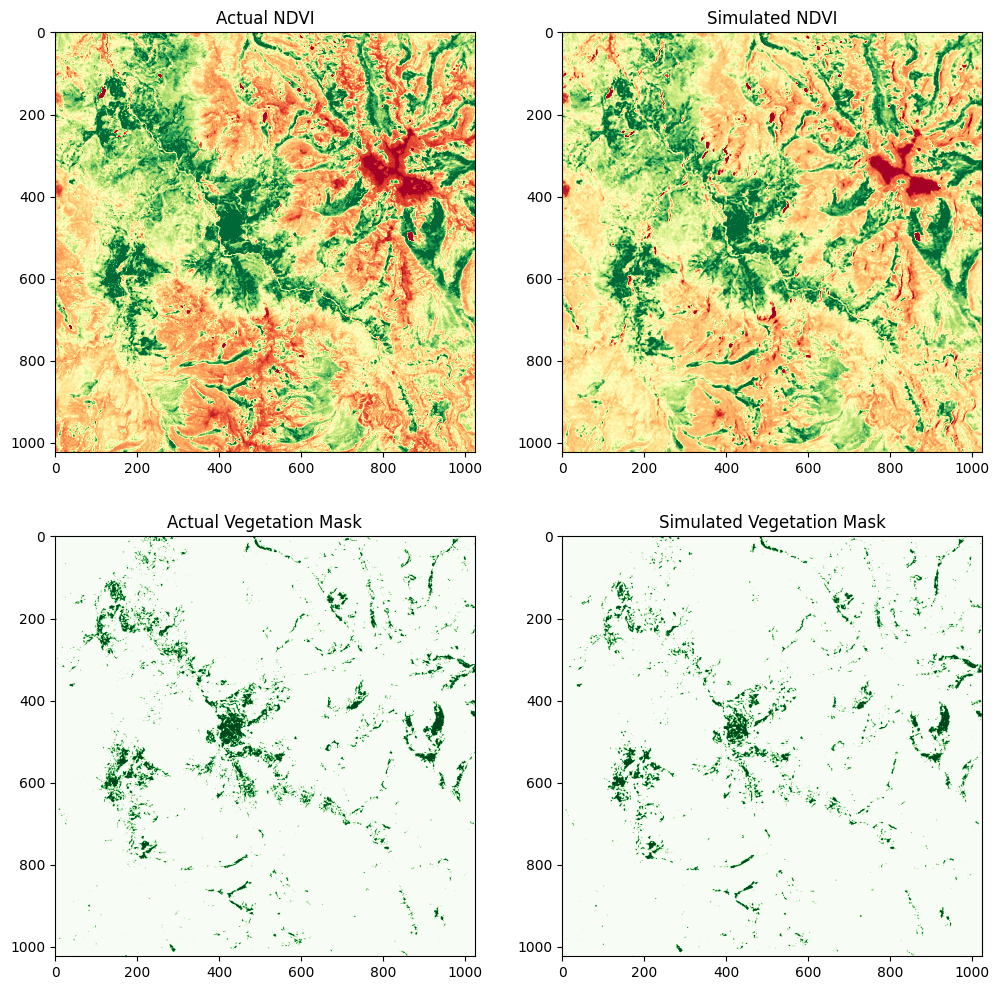
\includegraphics[width=1\linewidth]{2_CAPITULO5/IMG/ndvi2.png}
                        \begin{justify}
                            \textit{Nota.} La comparación de NDVI muestra cómo la vegetación es representada en las imágenes originales y simuladas, destacando la efectividad de la armonización espectral en la detección precisa de la vegetación.
                        \end{justify}                    
                        \label{ndvi2}
                    \end{figure}
        

                \paragraph{Índice de diferencia normalizada de agua (NDWI)}
                    El NDWI es útil para la detección de cuerpos de agua y se calcula usando las bandas verde (Green) y del infrarrojo cercano (NIR):

                    \begin{equation}
                        NDWI = \frac{\text{Green} - \text{NIR}}{\text{Green} + \text{NIR}}
                    \end{equation}

                    \begin{figure}[H] 
                        \caption{\doublespacing \\ \textit{Comparación de NDWI entre imágenes originales y simuladas.}} 
                        \centering
                        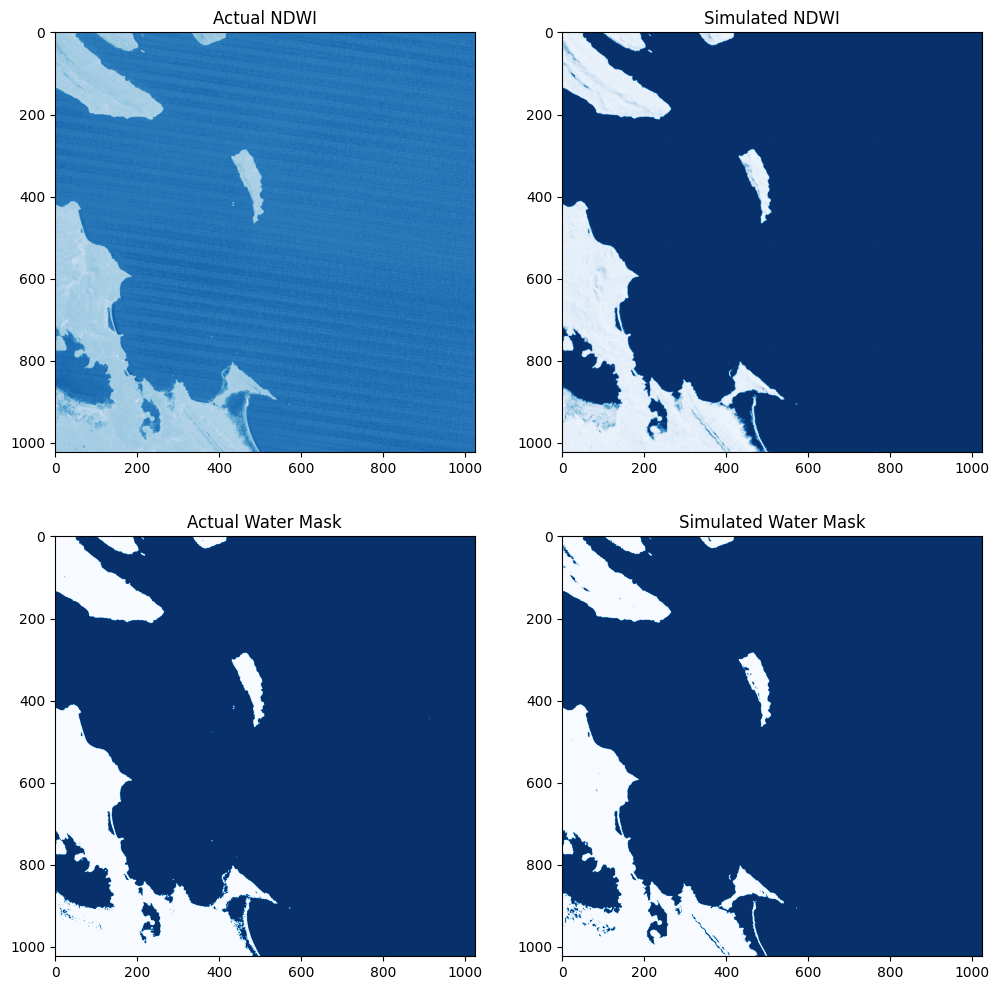
\includegraphics[width=1\linewidth]{2_CAPITULO5/IMG/ndwi.png}
                        \begin{justify}
                            \textit{Nota.} La comparación de NDWI muestra que el modelo detecta cuerpos de agua con mayor precisión en las imágenes simuladas, corrigiendo posibles errores en la banda verde de las imágenes actuales y mejorando la detección a pesar de las imperfecciones originales.
                        \end{justify}                    
                        \label{ndwi}
                    \end{figure}

                \paragraph{Índice de diferencia normalizada de nieve (NDSI)}
                    El NDSI es útil para la detección de nieve y se calcula usando las bandas verde (Green) y del infrarrojo de onda corta (SWIR):

                    \begin{equation}
                        NDSI = \frac{(Green - SWIR)}{(Green + SWIR)}
                    \end{equation}

                    \begin{figure}[H] 
                        \caption{\doublespacing \\ \textit{Comparación de NDSI entre imágenes originales y simuladas.}} 
                        \centering
                        \includegraphics[width=1\linewidth]{2_CAPITULO5/IMG/ndsi2.png}
                        \begin{justify}
                            \textit{Nota.} La comparación de NDSI evidencia la capacidad del modelo para detectar áreas nevadas con precisión en las imágenes simuladas en comparación con las originales.
                        \end{justify}                    
                        \label{ndsi2}
                    \end{figure}
        
    \section{Análisis estadístico de los resultados}
        \subsection{Contexto y metodología de Validación}

            \begin{figure}[H] 
                \caption{\doublespacing \\ \textit{Áreas de validación en Perú.}} 
                \centering
                \includegraphics[width=0.8\linewidth]{2_CAPITULO5/IMG/imagenes_peru.png}
                \label{imagenes_peru}
                \begin{justify}
                    \textit{Nota.} Mapa de Perú mostrando puntos de muestreo para la validación de superresolución de imágenes MSS en diversas regiones geográficas.
                \end{justify}                    
                \label{modelo3}
            \end{figure}

            El Perú ha sido seleccionado como área de validación debido a su variada topografía y diversidad de ecosistemas, que van desde la costa del Pacífico hasta las alturas de los Andes, proporcionando un escenario desafiante para la superresolución satelital. Las imágenes MSS fueron transformadas a la resolución de las imágenes TM, utilizando un conjunto de validación compuesto por 23 pares de imágenes.
            
        \subsection{Evaluación cuantitativa de la superresolución}

            \begin{table}[H]
                \caption{\doublespacing \\ \textit{Métricas entre imágenes simuladas y reales por imagen (valores promedio).}}
                \begin{spacing}{8}
                    \fontsize{8pt}{2pt}\selectfont  
                    \begin{tabularx}{\linewidth}{*{4}{X}} 
                        \toprule
                        \textbf{Imagen} & \textbf{MAE} & \textbf{RMSE} & \textbf{Coeficiente de Pearson} \\ 
                        \midrule
                        00031 & 0.150 & 0.200 & 0.750 \\ 
                        00032 & 0.146 & 0.196 & 0.740 \\ 
                        00074 & 0.148 & 0.198 & 0.745 \\
                        00213 & 0.147 & 0.197 & 0.735 \\ 
                        00273 & 0.150 & 0.200 & 0.750 \\
                        00328 & 0.147 & 0.197 & 0.755 \\ 
                        00353 & 0.151 & 0.201 & 0.725 \\ 
                        01145 & 0.148 & 0.198 & 0.740 \\
                        01440 & 0.149 & 0.199 & 0.750 \\ 
                        01465 & 0.148 & 0.198 & 0.745 \\ 
                        04590 & 0.149 & 0.199 & 0.740 \\ 
                        05720 & 0.150 & 0.200 & 0.750 \\ 
                        05883 & 0.147 & 0.197 & 0.730 \\ 
                        05826 & 0.150 & 0.200 & 0.745 \\ 
                        04706 & 0.149 & 0.199 & 0.740 \\ 
                        06008 & 0.153 & 0.203 & 0.725 \\ 
                        05935 & 0.150 & 0.200 & 0.745 \\ 
                        11030 & 0.149 & 0.199 & 0.740 \\ 
                        08849 & 0.151 & 0.201 & 0.725 \\ 
                        08927 & 0.149 & 0.199 & 0.740 \\ 
                        08929 & 0.148 & 0.198 & 0.740 \\ 
                        06776 & 0.150 & 0.200 & 0.750 \\ 
                        11281 & 0.152 & 0.202 & 0.720 \\ 
                        \bottomrule
                    \end{tabularx}
                \end{spacing}
                \vspace{1\baselineskip}
                \textit{Nota.} Evaluación detallada de la precisión de las imágenes transformadas en comparación con las originales, con un enfoque en la correlación lineal, error absoluto medio y error cuadrático medio.
                \label{valores_metricas}
            \end{table}
            
            \subsubsection{Interpretación de métricas:}

            Las métricas MAE y RMSE proporcionan una medida del error en las predicciones, siendo valores más bajos indicativos de mayor precisión. Por otro lado, el Coeficiente de Pearson destaca la correlación lineal entre los valores predichos y los reales, con valores cercanos a 1 denotando una alta precisión en la replicación de las tendencias de los datos originales.

        \subsection{Análisis detallado por bandas espectrales}

            \begin{table}[H]
                \caption{\doublespacing \\ \textit{Métricas por bandas entre imágenes simuladas y reales.}}
                \begin{spacing}{8}
                    \fontsize{8pt}{2pt}\selectfont  
                    \begin{tabularx}{\linewidth}{*{4}{X}} 
                        \toprule
                        \textbf{Banda} & \textbf{MAE} & \textbf{RMSE} & \textbf{Coeficiente de Pearson} \\ 
                        \midrule
                        \textbf{Make prediction - I} & & & \\
                        Green & 0.120 & 0.180 & 0.830 \\ 
                        Red & 0.080 & 0.130 & 0.890 \\ 
                        NIR & 0.075 & 0.120 & 0.880 \\
                        \midrule
                        \textbf{Generate bands - II} & & & \\
                        Blue & 0.090 & 0.140 & 0.860 \\ 
                        Green & 0.100 & 0.160 & 0.870 \\ 
                        Red & 0.110 & 0.170 & 0.880 \\ 
                        NIR & 0.125 & 0.190 & 0.850 \\ 
                        SWIR1 & 0.240 & 0.210 & 0.680 \\ 
                        Thermal & 0.650 & 0.900 & 0.120 \\ 
                        SWIR2 & 0.230 & 0.200 & 0.550 \\ 
                        \bottomrule
                    \end{tabularx}
                \end{spacing}
                \vspace{1\baselineskip}
                \textit{Nota.} Evaluación del rendimiento del modelo por banda espectral, mostrando cómo varía la precisión en diferentes rangos del espectro.
                \label{valores_metricas2}
            \end{table}
            
            Esta tabla proporciona una comparativa detallada de cómo el modelo performa en diferentes bandas espectrales, resaltando desafíos específicos como los observados en la banda térmica.

        \subsection{Distribución de métricas y variabilidad del modelo}    

            \begin{figure}[H] 
                \caption{\doublespacing \\ \textit{Distribución de métricas de validación.}} 
                \centering
                \includegraphics[width=1\linewidth]{2_CAPITULO5/IMG/box.jpeg}
                \begin{justify}
                    \textit{Nota.} Diagrama de cajas que muestra la variabilidad y dispersión de MAE, RMSE y coeficiente de Pearson en superresolución de imágenes MSS.
                \end{justify}                    
                \label{modelo}
            \end{figure}


            El diagrama de cajas proporciona una visión clara de la distribución estadística de las métricas de validación aplicadas a la superresolución de imágenes MSS en Perú. Cada métrica revela aspectos distintos de la precisión del modelo MSS2TM. El MAE destaca la exactitud media en la estimación de valores de píxeles, el RMSE señala la dispersión general de los errores en las predicciones del modelo, y el coeficiente de Pearson mide la fuerza y la dirección de la relación lineal entre las imágenes generadas y las originales.

            Los valores promedio de MAE y RMSE a lo largo de todas las imágenes evaluadas fueron 0.150 y 0.200, respectivamente, lo que indica un buen rendimiento general del modelo en el contexto de la superresolución. Sin embargo, hubo variabilidad en el rendimiento entre diferentes áreas, como lo demuestra el rango de valores de MAE y RMSE. La imagen identificada como 00328 mostró un desempeño sobresaliente con el MAE más bajo y el coeficiente de correlación de Pearson más alto, mientras que la imagen 06008 presentó los valores más altos de MAE y RMSE, además de la correlación más baja, lo que sugiere que ciertas áreas pueden presentar desafíos específicos para el modelo.

            Este análisis detallado permite no solo verificar la capacidad del modelo para generar imágenes TM de alta fidelidad a partir de imágenes MSS, sino también identificar áreas donde el modelo puede requerir ajustes o entrenamiento adicional para manejar condiciones específicas del paisaje.


        \subsection{Análisis de las bandas SWIR y térmica}

            Uno de los hallazgos más intrigantes de este estudio es el comportamiento particular de las bandas SWIR y térmica en las métricas de validación. Como se observa en la Tabla \ref{valores_metricas2}, estas bandas presentan un MAE y RMSE notablemente superiores a las demás, acompañados de coeficientes de Pearson significativamente más bajos, incluso negativos en el caso de la banda SWIR2. 

            Esta discrepancia se debe principalmente a las características únicas de estas bandas en comparación con las bandas ópticas. Mientras que las bandas ópticas, como el rojo, verde, y NIR, reflejan la radiación solar, las bandas SWIR y térmica miden la radiación infrarroja emitida por los objetos, lo cual es altamente influenciado por la temperatura superficial terrestre y las condiciones ambientales.

            La sensibilidad de las bandas SWIR y térmica a la variabilidad de las condiciones ambientales, como la temperatura y la humedad, puede aumentar los errores de predicción cuando se utilizan modelos entrenados predominantemente en bandas ópticas. Este fenómeno es particularmente pronunciado en áreas con diversidad geográfica y climática como Perú, donde la variación de la temperatura superficial puede ser extrema debido a la topografía variada del país.

            La baja autocorrelación espectral de estas bandas también contribuye a la dificultad en su predicción. A diferencia de las bandas ópticas, donde la correlación entre bandas puede ser explotada para mejorar la precisión de la predicción, las bandas SWIR y térmica frecuentemente no muestran una correlación directa con otras bandas, lo que resulta en un desafío mayor para los algoritmos de superresolución que dependen de estas correlaciones para generar predicciones precisas.

            Este análisis refuerza la importancia de desarrollar estrategias específicas para la armonización y superresolución de las bandas SWIR y térmica, posiblemente a través de la integración de modelos que incorporen variables ambientales y terrestres que afectan directamente a las mediciones en estas bandas.

        
        
        
% % \Chapter{}
% % \chapter{PRESUPUESTO}
% %     \begin{table}[H]
% %         \caption{\doublespacing \\ \textit{Presupuesto detallado para el proyecto de investigación.}}
% %         \begin{spacing}{1.5}
% %             \fontsize{8pt}{10pt}\selectfont  
% %             \begin{tabularx}{\linewidth}{*{4}{P{4.5cm}}} 
% %                 \toprule
% %                 \multicolumn{4}{c}{\textbf{Presupuesto total (Montos aproximados en S/.)}} \\ 
% %                 \midrule
% %                 \textbf{Rubro} & \textbf{Costo unitario} & \textbf{Cantidad} & \textbf{Total} \\
% %                 \midrule
% %                 Equipos: & & & \\ 
% %                 Laptop & 3000 & 1 & 3000 \\ 
% %                 Disco duro de 1 Tbyte & 200 & 1 & 200 \\ 
% %                 Internet: & & & \\ 
% %                 Servicio de internet (12 meses) & 1400 & 1 & 1400 \\
% %                 Papelería y útiles: & & & \\
% %                 Materiales de escritorio & 150 & 1 & 150 \\ 
% %                 Impresiones & 800 & 1 & 800 \\ 
% %                 Software: & & & \\ 
% %                 QGIS, Python, R (gratuitos) & 0 & 1 & 0 \\ 
% %                 \midrule
% %                 Tiempo de investigación: & & & \\
% %                 Medio sueldo mínimo mensual & 512.5 & 12 & 6150 \\
% %                 \midrule
% %                 \textbf{Total General:} & & & \textbf{11700} \\
% %                 \bottomrule
% %             \end{tabularx}
% %         \end{spacing}
% %         \vspace{1\baselineskip}
% %         \textit{Nota.} El presupuesto incluye equipamiento, servicios, materiales y el costo estimado del tiempo del investigador basado en medio sueldo mínimo mensual, reflejando la dedicación parcial al proyecto durante un año. No incluye otros posibles gastos indirectos o costos de oportunidad.
% %         \label{Presupuesto}
% %     \end{table}


	% \Chapter{}

% \chapter{CRONOGRAMA DE ACTIVIDADES}
%     \begin{figure}[H] 
%         \caption{\doublespacing \\ \textit{Cronograma de actividades para la investigación.}} 
%         \centering
%         \includegraphics[width=1.12\linewidth, angle=90]{2_CAPITULO0/IMG/cronograma.png}
%         \begin{justify}
%             \textit{Nota.} El cronograma anual detalla la secuencia de actividades, desde la elección de imágenes Landsat hasta las modificaciones finales, organizadas semanalmente a lo largo de un año.
%         \end{justify}                    
%         \label{cronograma}
%     \end{figure}

\chapter{DISCUSIÓN}

    La validación cuantitativa del modelo SWINIR - MSS2TM se centró en la precisión espectral y la superresolución, destacando la selección estratégica de Perú por su diversidad topográfica y ecosistémica. Comparado con estudios previos en el campo, este modelo demostró un rendimiento competitivo y estuvo en línea con los avances más recientes en la literatura científica relacionada con la superresolución y la armonización de imágenes satelitales .

    \section{Evaluación comparativa con estudios previos}
        Los resultados obtenidos indicaron que el modelo SWINIR - MSS2TM no solo mejoró la alineación espacial de las imágenes MSS respecto a las TM, sino que también optimizó la armonización espectral, como lo demostraron las mejoras significativas en los índices espectrales NDVI, NDWI y NDSI. Estos avances fueron comparables, si no superiores, a los logrados en estudios similares recientes, destacando el potencial de las técnicas de aprendizaje profundo en el procesamiento de imágenes satelitales .

    \section{Variabilidad geográfica y rendimiento del modelo}
        A pesar del buen rendimiento general del modelo, evidenciado por las métricas de MAE, RMSE y el coeficiente de Pearson, se observaron variaciones notables en la efectividad de la superresolución entre diferentes regiones geográficas. Específicamente, los resultados subóptimos en la imagen 06008, ubicada sobre el Lago Titicaca, destacaron los desafíos asociados con cuerpos de agua, donde la interferencia atmosférica y la homogeneidad espectral pueden degradar la precisión del modelo. Este fenómeno sugirió que el modelo podría beneficiarse de ajustes o configuraciones específicas cuando se enfrenta a condiciones espectralmente homogéneas o interferencias atmosféricas.

    \section{Implicaciones prácticas y limitaciones}
        Las implicaciones prácticas de los resultados fueron considerablemente positivas, particularmente para aplicaciones que demandan alta fidelidad en la interpretación de datos satelitales. La capacidad del modelo para mejorar la resolución y precisión espectral de las imágenes MSS facilitó aplicaciones en cartografía, gestión de recursos naturales y monitorización ambiental. Sin embargo, las limitaciones observadas en cuerpos de agua y bajo condiciones atmosféricas adversas requirieron un enfoque más especializado. La integración de métodos que pudieran compensar estas condiciones podría mejorar sustancialmente la versatilidad y la eficacia del modelo .


	% \chapter{CONCLUSIONES Y RECOMENDACIONES}
    \section{Conclusiones}
        Esta investigación demostró con éxito la capacidad del modelo SWINIR - MSS2TM para armonizar las características espectrales y espaciales de las imágenes MSS con las imágenes TM. La integración de técnicas de aprendizaje profundo y procesamiento de imágenes mejoró significativamente la corrección geométrica de las imágenes Landsat MSS, logrando una superposición casi perfecta con las imágenes TM. Este avance es crucial para la estandarización de datos satelitales, facilitando análisis más consistentes y confiables a largo plazo.

        Se comprobó que la alineación precisa tanto espectral como espacial entre las imágenes Landsat MSS y TM fue alcanzada mediante el modelo MSS2TM. Las mejoras significativas en los índices espectrales como NDVI, NDWI y NDSI destacaron la efectividad del modelo en la armonización espectral, demostrando su capacidad para detectar con precisión la vegetación, cuerpos de agua y áreas nevadas.
        
        Adicionalmente, se verificó la viabilidad de complementar las imágenes MSS con bandas espectrales adicionales a través de modelos de aprendizaje profundo. Este enriquecimiento de las imágenes MSS amplió su aplicabilidad en campos que demandan alta precisión espectral, mejorando la calidad y utilidad de los datos históricos de Landsat MSS. Sin embargo, se concluye que todavía existe un margen de mejora, especialmente en la armonización de las bandas térmicas y SWIR, las cuales no se logran replicar con la misma efectividad que las bandas ópticas como la azul. Esto es particularmente importante para la corrección atmosférica y otras aplicaciones avanzadas.
        
        La validación del modelo en una región geográficamente diversa como Perú demostró su robustez y capacidad de generalización, resaltando la importancia de adaptar el modelo a las variaciones específicas de cada zona de interés.
    
    \section{Recomendaciones}
        Basado en los hallazgos y logros de esta tesis, se recomienda lo siguiente para futuras investigaciones en el campo de la armonización de imágenes satelitales:

        \begin{enumerate}
            \item \textbf{Explorar nuevas arquitecturas de redes neuronales:} Continuar el desarrollo y la experimentación con arquitecturas innovadoras, como los Transformers y GANs avanzados, para mejorar aún más la calidad de la armonización espectral y la generación de bandas virtuales.
            \item \textbf{Diversificar los conjuntos de datos:} Ampliar los conjuntos de datos utilizados para incluir imágenes de una gama más amplia de condiciones ambientales y geográficas. Esto permitirá evaluar con mayor profundidad la robustez y generalizabilidad de los modelos propuestos.
            \item \textbf{Desarrollar herramientas integrables:} Crear herramientas de armonización automatizadas que puedan integrarse fácilmente con sistemas de información geográfica existentes, facilitando la aplicación práctica de los modelos en áreas como la agricultura, el urbanismo y la monitorización del cambio climático.
            \item \textbf{Fomentar la colaboración interdisciplinaria:} Publicar el código fuente y los conjuntos de datos en plataformas de acceso abierto para potenciar la colaboración interdisciplinaria y acelerar la adopción de estas tecnologías avanzadas en la comunidad científica y profesional.
            \item \textbf{Explorar técnicas adicionales:} Adaptar los modelos para manejar variaciones espectralmente homogéneas y la interferencia atmosférica, desarrollando algoritmos que ajusten dinámicamente los parámetros del modelo en función de las características específicas de cada área geográfica. La investigación futura también debería centrarse en la superresolución de la banda térmica para mejorar la precisión en aplicaciones de teledetección.
        \end{enumerate}


	% % FUNDAMENTO TEÓRICO Y CONCEPTUAL
	% \chapter{FUNDAMENTO TEÓRICO Y CONCEPTUAL}
\markboth{CAPÍTULO \thechapter: MARCO TEÓRICO Y CONCEPTUAL}{}

\lipsum[23]

	\section{PRIMER TEMA}
	\subsection{Aisladores Sísmicos}
Son dispositivos que desacoplan la estructura y su contenido de los efectos de un sismo. Este desacople se alcanza incrementando la flexibilidad del sistema y proporcionándole un amortiguamiento adecuado \shortcites{Skinner1993}\citep{Skinner1993}.

Existen diversos tipos de aisladores sísmicos, siendo los más usados en la actualidad los aisladores elastoméricos y los aisladores friccionantes.

		\subsubsection{Aisladores Elastoméricos}
\begin{itemize}

\item Aisladores de elastómero natural o de bajo amortiguamiento

Los dispositivos NRB (\textit{Natural Rubber Bearing}) consisten en capas alternadas de caucho y acero unidas mediante un proceso de vulcanización. Se caracterizan por su bajo nivel de amortiguamiento (alrededor de 2-3\%), poseen una curva fuerza deformación casi lineal y una fuerza restitutiva estable \citep{Kelly1999}.

\end{itemize}

		\subsubsection{Aisladores Friccionantes}
\begin{itemize}

\item Aisladores de péndulo de fricción simple

Los dispositivos FPS (\textit{Frictional Pendulum System}) constan de un deslizador articulado que se mueve sobre una superficie de fricción esférica. La superficie de contacto está revestida de un material compuesto autolubricante. Cuando el deslizador se mueve sobre la superficie esférica, la masa soportada se levantará y el movimiento proporcionará la fuerza restitutiva del sistema. El radio de curvatura de la superficie cóncava dominará la rigidez y el periodo del sistema \citep{Wu2001}.

\end{itemize}


	\begin{figure}[!h]
	\centering
	\begin{subfigure}[b]{0.45\textwidth}
  	\centering
  	% include first image
  	\includegraphics[scale=1]{E_IMAGENES/1_Capitulo2/Cap2_Imagen1a.pdf}
 	\caption{\centering\footnotesize Aislador eslastomérico LRB. Adaptado de \citet{Bridgestone2015}}
  	\label{Cap2_Figura1a}
	\end{subfigure}
	\hfill
	\begin{subfigure}[b]{0.45\textwidth}
  	\centering
  	% include second image
  	\includegraphics[scale=1]{E_IMAGENES/1_Capitulo2/Cap2_Imagen1b.pdf} 
  	\caption{\centering\footnotesize Aislador friccionante TFPB. Adaptado de \citet{Fenz2008}}
  	\label{Cap2_Figura1b}
	\end{subfigure}
	\caption[Dispositivos de aislamiento sísmico]{\centering\footnotesize Dispositivos de aislamiento sísmico}
	\label{Cap2_Figura1}
	\end{figure}
	
	\subsection{Disipadores de Fluido Viscoso}
Son dispositivos que incrementan el amortiguamiento de la estructura sin incrementar la rigidez y cuyo funcionamiento depende fundamentalmente de la velocidad relativa de sus extremos. Los DFV están compuestos por un pistón de acero inoxidable, con cabezal de bronce y un acumulador, que se encuentran alojados dentro en un cilindro metálico lleno con un fluido de alta viscosidad. La cabeza del pistón tiene orificios que están diseñados con una serie de formas especiales para alterar las características de flujo con la velocidad del fluido, disipando de esta manera energía en forma de calor. La construcción mecánica y las propiedades del orificio se pueden variar para obtener las propiedades amortiguadoras deseadas \citep{Constantinou1993}.

	\begin{figure}[!h]
	\centering
		\includegraphics[scale=1]{E_IMAGENES/1_Capitulo2/Cap2_Imagen2.pdf}
	\caption[Disipador de fluido viscoso]{\centering\footnotesize Disipador de fluido viscoso.  Adaptado de \shortcites{Taylor2019}\citet{Taylor2019}}
	\label{Cap2_Figura2}
	\end{figure}
	
	
	
	


	\section{SEGUNDO TEMA}

En esta sección se revisan modelos matemáticos capaces de describir de forma analítica una amplia gama de comportamientos inelásticos complejos presentes en muchos sistemas y materiales.

	\subsection{Modelo Histerético de Bouc-Wen} \label{subsection:MHBW}
	
Es un modelo que se usa para predecir el comportamiento dinámico no lineal de aisladores sísmicos, así como de disipadores histeréticos. El modelo de Bouc-Wen necesita cuatro parámetros de entrada, los cuales son: la rigidez elástica, la rigidez postfluencia, la fuerza característica y un parámetro adimensional que controla la forma del lazo histerético.

De acuerdo con \citet{Charalampakis2010} la fuerza en el tiempo \textit{t} del modelo histerético de Bouc-Wen se evalúa en función del desplazamiento de la siguiente manera:
\begin{gather}
F(t)=\alpha \frac{F_{y}}{D_{y}}u(t)+(1-\alpha)F_{y}z(t)				\label{BoucWen1} \\
\begin{aligned}
\dot{z}(t)=\left[1-\left|z(t)\right |^{\eta}sgn(\dot{u}(t)z(t))\right]\frac{\dot{u}(t)}{D_{y}}&,&\hspace{1em}& z(0)=0 \\
\end{aligned}		\label{BoucWen2}
\end{gather}

	\begin{figure}[!h]
	\centering
		\includegraphics[scale=1]{E_IMAGENES/1_Capitulo2/Cap2_Imagen6.pdf}
		%\vspace{-3 mm}
	\caption[Modelo histerético de Bouc-Wen]{\centering\footnotesize Modelo histerético de Bouc-Wen. Adaptado de \citet{Charalampakis2010}}
	\label{Cap2_Figura6}
	\end{figure}

En la \autoref{Cap2_Figura6} y en las ecuaciones \ref{BoucWen1} y \ref{BoucWen2} se muestran los parámetros necesarios para definir un ciclo histerético con comportamiento de Bouc-Wen.

Donde:

%Inicar tabla explicando cada Parámetro
\begin{tabular}{L{0.5 cm}p{0.025 cm}p{11.5 cm}}
  $K_{e}$ & : & Rigidez elástica \\
  $K_{p}$ & : & Rigidez postfluencia \\
  $Q$     & : & Fuerza característica \\
  $D_{y}$ & : & Desplazamiento de fluencia \\
  $F_{y}$ & : & Fuerza de fluencia \\
  $\alpha$ & : & Razón entre la rigidez postfluencia y la rigidez elástica  \\
  $\eta$ & : & Parámetro adimensional que controla la forma del lazo histerético \\
 \end{tabular}\\

	
 
 
	
	\section{TERCER TEMA}
 
	\subsection{Modelo de Masas Concentradas}
	
Es un modelo físico discreto conformado por una serie de masas interconectadas por resortes sin peso (sistema de acoplamiento cercano). Este modelo puede describir adecuadamente el comportamiento de edificaciones con un sistemas estructural basado en pórticos con vigas muy rígidas y donde las deformaciones axiales de las columnas se desprecian.

		\subsubsection{Matrices de Masa y Rigidez}

Para un modelo discreto de masas concentradas de $n$ GDL, la matriz de masas $\mathbfit{M}$ es diagonal, con la masa $i_{\acute{e}sima}$, $m_{i}$, como el elemento diagonal $i_{\acute{e}simo}$.

\begin{equation}\label{Eq18}
M=\begin{bmatrix}
m_{1} & 0 & 0 & \cdots & 0 & 0 \\ 
0 & m_{2} & 0 & \cdots & 0 & 0\\ 
0 & 0 & m_{3} & \cdots & 0 & 0\\ 
\vdots & \vdots & \vdots &\ddots  &\vdots  &\vdots \\ 
0 & 0 & 0 & \cdots & m_{n-1}& 0\\ 
0 & 0 & 0 & \cdots & 0 & m_{n}
\end{bmatrix}_{n\times n}
\end{equation}



		\subsubsection{Matriz de Amortiguamiento}

Usando el amortiguamiento de Rayleigh se puede construir una matriz de amortiguamiento que sea consisten con los datos experimentales \citep{Chopra2016}. Tal como se aprecia en la ecuación \ref{Eq21}, Rayleigh propone que la matriz de amortiguamiento sea una combinación lineal de la matriz de masa y la matriz de rigidez.
\begin{equation}\label{Eq21}
\mathbfit{C}=a_{0}\mathbfit{M}+a_{1}\mathbfit{K}
\end{equation}







	
	\section{CUARTO TEMA}

De acuerdo con la ASCE 7-16 y la norma E.031 cuando se realice un análisis tiempo historia para diseñar edificaciones que incorporen algún sistema de control pasivo se debe usar un mínimo de siete registros sísmico, los cuales deben estar escalados correctamente. Dado que el objetivo de la presente tesis no es realizar un diseño detallado sino más bien conocer la eficiencia de cada sistema de control pasivo en la reducción de la respuesta sísmica, se usaron solo tres registros.

	\subsection{Registros Sísmicos Ajustados}
	
A continuación se presentan los registros sísmicos usados en la presente tesis.
			
	\begin{figure}[h!]
	\centering
	\includegraphics[scale=1]{E_IMAGENES/1_Capitulo2/Cap2_PiscoSc.pdf}
	\vspace{-8 mm}
	\caption[Acelerogramas espectrocompatibles - Pisco 2007]{\centering\footnotesize Acelerogramas espectrocompatibles - Pisco 2007.}
	\label{Cap2_Figura15}
	\end{figure}	
			

	


	
		
	% % CAPÍTULO 3
	% \chapter{NOMBRE DEL CAPÍTULO 3}
\markboth{CAPÍTULO \thechapter: NOMBRE DEL CAPÍTULO 3}{}

\lipsum [6]

	\input{2_CAPITULO3/Secciones/1_Primera Sección.tex}
	
	\input{2_CAPITULO3/Secciones/2_Segunda Sección.tex}
	
	\input{2_CAPITULO3/Secciones/3_Tercera Sección.tex}
	
	\input{2_CAPITULO3/Secciones/4_Cuarta Sección.tex}




		


		
	% % CAPÍTULO 4
	% \chapter[NOMBRE DEL CAPÍTULO 4]{NOMBRE DEL CAPÍTULO 4}
\markboth{CAPÍTULO \thechapter: NOMBRE DEL CAPÍTULO 4}{}

\lipsum[10]

	\input{2_CAPITULO4/Secciones/1_Primera Sección.tex}
	
	\input{2_CAPITULO4/Secciones/2_Segunda Sección.tex}
	




		

		
	
	% %Parte FINAL DE LA TESIS
	
	% \backmatter

	% % CONCLUSIONES
	% \cleardoublepage\phantomsection\addcontentsline{toc}{chapter}{\bf CONCLUSIONES}
\chapter*{\centerline {CONCLUSIONES}}
\markboth{CONCLUSIONES}{}
%--
\begin{enumerate}

\item Nam dui ligula, fringilla a, euismod sodales, sollicitudin vel, wisi.  Morbiauctor lorem non justo. Nam lacus libero, pretium at, lobortis vitae, ultricies et,tellus. Donec aliquet, tortor sed accumsan bibendum, erat ligula aliquet magna,vitae ornare odio metus a mi.

\item Nam dui ligula, fringilla a, euismod sodales, sollicitudin vel, wisi.  Morbiauctor lorem non justo. Nam lacus libero, pretium at, lobortis vitae, ultricies et,tellus. Donec aliquet, tortor sed accumsan bibendum, erat ligula aliquet magna,vitae ornare odio metus a mi.

\item Nam dui ligula, fringilla a, euismod sodales, sollicitudin vel, wisi.  Morbiauctor lorem non justo. Nam lacus libero, pretium at, lobortis vitae, ultricies et,tellus. Donec aliquet, tortor sed accumsan bibendum, erat ligula aliquet magna,vitae ornare odio metus a mi.


\end{enumerate}

	
	% % RECOMENDACIONES	
	% \cleardoublepage\phantomsection\addcontentsline{toc}{chapter}{\bf RECOMENDACIONES}
\chapter*{\centerline {RECOMENDACIONES}}
\markboth{RECOMENDACIONES}{}
%
\begin{enumerate}
\item Nam dui ligula, fringilla a, euismod sodales, sollicitudin vel, wisi.  Morbiauctor lorem non justo. Nam lacus libero, pretium at, lobortis vitae, ultricies et,tellus. Donec aliquet, tortor sed accumsan bibendum, erat ligula aliquet magna,vitae ornare odio metus a mi.

\item Nam dui ligula, fringilla a, euismod sodales, sollicitudin vel, wisi.  Morbiauctor lorem non justo. Nam lacus libero, pretium at, lobortis vitae, ultricies et,tellus. Donec aliquet, tortor sed accumsan bibendum, erat ligula aliquet magna,vitae ornare odio metus a mi.

\item Nam dui ligula, fringilla a, euismod sodales, sollicitudin vel, wisi.  Morbiauctor lorem non justo. Nam lacus libero, pretium at, lobortis vitae, ultricies et,tellus. Donec aliquet, tortor sed accumsan bibendum, erat ligula aliquet magna,vitae ornare odio metus a mi.


\end{enumerate}
	
	% REFERENCIAS BIBLIOGRÁFICAS
	% \cleardoublepage\phantomsection\addcontentsline{toc}{chapter}{\bf REFERENCIAS BIBLIOGRÁFICAS}
% \begingroup
% \titleformat*{\chapter}{\normalfont\bfseries\normalsize\centering}
% \bibliography{3_3_BIBLIOGRAFIA/library}
% \endgroup

\clearpage
\phantomsection
% \addcontentsline{toc}{chapter}{\bibname}
\printbibliography[heading=bibintoc, title={REFERENCIAS BIBLIOGRÁFICAS}]
	
	% ANEXOS	
	% \cleardoublepage\phantomsection\addcontentsline{toc}{chapter}{\bf ANEXOS}
\chapter*{\centerline {ANEXOS}}
\markboth{ANEXOS}{}
%---

% Definir númeración y citación para Listing 

\renewcommand{\lstlistingname}{ \footnotesize Código A \hspace{-1.75mm}}% Cambiar el nombre a Algoritmo
\renewcommand*{\thelstlisting}{.\arabic{lstlisting}} 
\def\lstlistingautorefname{Código A\hspace{-0.75mm}}

% Redefinir númeración y citación para Figuras
\renewcommand\thefigure{.\arabic{figure}}  
\setcounter{figure}{0} 
\renewcommand\figurename{\footnotesize FIGURA B \hspace{-1.6mm}}
\def\figureautorefname{Figura B \hspace{-2mm}}


	% \subsection*{Respuesta Sísmica de una Edificación con AS}
%\phantomsubsection
% \addcontentsline{toc}{subsection}{Respuesta Sísmica de una Edificación con AS}



\addcontentsline{toc}{section}{Operacionalización de variables}

\vspace*{2mm}

\begin{table}[H]
    \caption{\doublespacing \\ \textit{Operacionalización de variables}}
    \begin{spacing}{8}
        \fontsize{8pt}{2pt}\selectfont  
        \begin{tabularx}{\linewidth}{P{2.5cm}P{2.6cm}P{4cm}P{2.5cm}P{2.5cm}} % *{4}{P{3cm}}
            \toprule
            % \multicolumn{1}{c}{\textbf{Variables}} & \multicolumn{1}{c}{\textbf{Subvariables}} & \multicolumn{1}{c}{\textbf{Operacionalización}} & \multicolumn{1}{c}{\textbf{Unidad de medida}} & \multicolumn{1}{c}{\textbf{Instrumento}} \\
            \multicolumn{1}{c}{\textbf{Variables}} & \multicolumn{1}{c}{\textbf{Dimensiones}} & \multicolumn{1}{c}{\textbf{Indicadores}} & \multicolumn{1}{c}{\textbf{Unidad de medida}} & \multicolumn{1}{c}{\textbf{Instrumento}} \\
            \midrule
            Inteligencia artificial (independiente) & Corrección geométrica & Error RMS después del ajuste geométrico & Píxeles (px) & Python (LightGlue) \\
            \addlinespace
            & Alineación espectral & Coeficiente de correlación entre las imágenes MSS y TM armonizadas espacialmente & Coeficiente de correlación (r) & Python (Pytorch) \\
            \addlinespace
            & Generación de bandas faltantes & Número de bandas generadas para completar MSS comparable con TM & Número de bandas (nb) & Python (Pytorch) \\
            \addlinespace
            \addlinespace
            Armonización de imágenes satelitales (dependiente) & Precisión de alineación & Precisión de la superposición de píxeles en imágenes armonizadas & Metros (m) & Python (GDAL, Rasterio) \\
            \addlinespace
            & Similitud espectral & Índice de similitud espectral entre imágenes MSS y TM & Sin unidades & Python (PyTorch) \\
            \addlinespace
            & Resolución espacial & Resolución espacial de las imágenes armonizadas & Metros por píxel (m/px) & Python (Rasterio) \\
            \addlinespace
            & Integridad de datos temporales & Cobertura temporal completa en el cubo de datos armonizado & Porcentaje (\%) & Python (xarray) \\
            \bottomrule
        \end{tabularx}
    \end{spacing}
    \vspace{1\baselineskip}
    % \textit{Nota.} Esta tabla muestra las variables operacionalizadas, destacando cómo la inteligencia artificial contribuye a la armonización de imágenes satelitales con modelos de aprendizaje profundo reflejados en las subvariables y métricas, utilizando Python como instrumento clave de implementación.
    \textit{Nota.} Esta tabla muestra las variables operacionalizadas, destacando cómo la inteligencia artificial contribuye a la armonización de imágenes satelitales con modelos de aprendizaje profundo reflejados en las dimensiones y métricas, utilizando Python como instrumento clave de implementación.
    \label{UsoLandsat1}
\end{table}




\addcontentsline{toc}{section}{Matriz de consistencia}

\vspace*{2mm}

\begin{table}[H]
    \caption{\doublespacing \\ \textit{Matriz de consistencia.}}
    \centering
    \begin{spacing}{8}
        \fontsize{8pt}{2pt}\selectfont
        \begin{tabularx}{\textwidth}{@{}XXX@{}}
            \toprule
            \multicolumn{1}{c}{\textbf{Pregunta general}} & \multicolumn{1}{c}{\textbf{Objetivo general}} & \multicolumn{1}{c}{\textbf{Hipótesis general}} \\
            \midrule
            ¿Cómo armonizar las imágenes Landsat MSS para su uso en el monitoreo global y a largo plazo, utilizando inteligencia artificial? & Armonizar las imágenes Landsat MSS utilizando inteligencia artificial para su uso el monitoreo global y a largo plazo & El uso de inteligencia artificial para armonizar las imágenes Landsat MSS permitirá que adquieran propiedades de las imágenes TM, haciendo viable su uso en monitoreos globales de largo plazo \\
            \addlinespace
            \midrule
            \textbf{Preguntas específicas} & \textbf{Objetivos específicos} & \textbf{Hipótesis específicas} \\
            \midrule
            ¿Cómo integrar el aprendizaje profundo y procesamiento de imágenes en la corrección geométrica de las imágenes Landsat MSS y alinearlas con las TM a nivel de pixel y subpixel? & Integrar técnicas de aprendizaje profundo y procesamiento de imágenes para la corrección geométrica de las imágenes Landsat MSS, buscando una alineación precisa con las imágenes TM a niveles de pixel y sub-pixel & La integración de aprendizaje profundo y procesamiento de imágenes mejorará la corrección geométrica de las imágenes Landsat MSS, facilitando su armonización con las imágenes TM \\
            \addlinespace
            ¿De qué manera puede el modelo de aprendizaje profundo MSS2TM alinear espectral y espacialmente las imágenes Landsat MSS y TM? & Desarrollar el modelo de aprendizaje profundo MSS2TM para alinear espectral y espacialmente las imágenes Landsat MSS y TM & El modelo MSS2TM, basado en aprendizaje profundo, logrará una alineación precisa tanto espectral como espacial entre las imágenes Landsat MSS y TM \\
            \addlinespace
            ¿Mediante qué técnica de aprendizaje profundo se puede generar bandas faltantes en imágenes MSS que existen en las TM? & Implementar una técnica de aprendizaje profundo para generar bandas ausentes en imágenes MSS que existen en las TM & La técnica de aprendizaje profundo propuesta permitirá completar las bandas ausentes en las imágenes Landsat MSS, logrando una similitud significativa con las bandas presentes en las TM \\
            \bottomrule
        \end{tabularx}
    \end{spacing}
    \label{MatrizConsistencia}
\end{table}




% \begin{table}[H]
%     \caption{\doublespacing \\ \textit{Comparación y visualización de bandas y longitudes de onda de sensores Landsat mediante Spectral Viewer del U.S. Geological Survey.}}
%     \begin{spacing}{8}
%         \fontsize{8pt}{2pt}\selectfont  
%         \begin{tabularx}{\linewidth}{P{3cm}*{10}{c}} 
%             \toprule
%             \textbf{Designaciones de banda} & \multicolumn{2}{c}{\textbf{L8-9 OLI/TIRS}} & \multicolumn{2}{c}{\textbf{L7 ETM+}} & \multicolumn{2}{c}{\textbf{L4-5 TM}} & \multicolumn{2}{c}{\textbf{L4-5 MSS*}} & \multicolumn{2}{c}{\textbf{L1-3 MSS*}} \\
%             \midrule
%             & B & Longitud & B & Longitud & B & Longitud & B & Longitud & B & Longitud \\
%             \midrule
%             Costera/Aerosol & 1 & 0.43–0.45 & -- & -- & -- & -- & -- & -- & -- & -- \\
%             Azul & 2 & 0.45–0.51 & 1 & 0.45–0.52 & 1 & 0.45–0.52 & -- & -- & -- & -- \\
%             Verde & 3 & 0.53–0.59 & 2 & 0.52–0.60 & 2 & 0.52–0.60 & 1 & 0.5–0.6 & 4 & 0.5–0.6 \\
%             Pancromática** & 8  & 0.50–0.68 & 8 & 0.52–0.90 & -- & -- & -- & -- & -- & -- \\
%             Rojo & 4 & 0.64–0.67 & 3 & 0.63–0.69 & 3 & 0.63–0.69 & 2 & 0.6–0.7 & 5 & 0.6–0.7 \\
%             Infrarrojo cercano & 5 & 0.85–0.88 & 4 & 0.77–0.90 & 4 & 0.76–0.90 & 3 & 0.7–0.8 & 6 & 0.7–0.8 \\
%             Infrarrojo cercano & -- & -- & -- & -- & -- & -- & 4 & 0.8–1.1 & 7 & 0.8–1.1 \\
%             Cirrus & 9 & 1.36–1.38 & -- & -- & -- & -- & -- & -- & -- & -- \\
%             Infrarrojo corto-1 & 6 & 1.57–1.65 & 5 & 1.55–1.75 & 5 & 1.55–1.75 & -- & -- & -- & -- \\
%             Infrarrojo corto-2 & 7 & 2.11–2.29 & 7 & 2.09–2.35 & 7 & 2.08–2.35 & -- & -- & -- & -- \\
%             Térmico & 10 T1 & 10.60–11.19 & 6 T2 & 10.40–12.50 & 6 T2 & 10.40–12.50 & -- & -- & -- & -- \\
%             Térmico & 11 T1 & 11.50–12.51 & -- & -- & -- & -- & -- & -- & -- & -- \\
%             \bottomrule
%         \end{tabularx}
%     \end{spacing}
%     \vspace{1\baselineskip}
%     \textit{Nota.} Hay observaciones que se debe tener en cuenta. Adapatado de \textcite{Landsat2023}. \\
%         * Adquirido a 80 metros, remuestreado a 60 metros. \\
%         ** 15 metros (pancromático). \\
%         T1 = Térmico (adquirido a 100 metros, remuestreado a 30 metros). \\
%         T2 = Térmico (adquirido a 120 metros, remuestreado a 30 metros). 
%     \label{BandasLandsat}
% \end{table}
	% \newpage

	% \section*{ANEXO B: HISTÉRESIS DE LOS DISPOSITIVOS DE CONTROL}
\phantomsection
\addcontentsline{toc}{section}{ANEXO B: HISTÉRESIS DE LOS DISPOSITIVOS DE CONTROL}

\lipsum[10]

	\subsection*{Edificio Principal del Aeropuerto Jorge Chavez}
%\phantomsubsection
\addcontentsline{toc}{subsection}{Edificio Principal del Aeropuerto Jorge Chavez}

La \autoref{Anexo_1} muestra las histéresis de uno de los dos los DFV instalados en el eje 5-5 del primer nivel del edificio pincipal del aeropuerto Jorge Chavez. Asimismo, la \autoref{Anexo_2} presenta la histéresis de uno de los tres DH-SLB colocado en el eje 5-5 del primer nivel de la misma edificación.


	\begin{figure}[!h]
	\centering
	\includegraphics[scale=1]{E_IMAGENES/Anexos/Anexo_1.pdf}
	\vspace{-8 mm}
	\caption[]{\centering\footnotesize Histéresis del DFV del edificio del aeropuerto Jorge Chavez.}
	\label{Anexo_1}
	\end{figure}	


	\begin{figure}[!h]
	\centering
	\includegraphics[scale=1]{E_IMAGENES/Anexos/Anexo_2.pdf}
	\vspace{-8 mm}
	\caption[]{\centering\footnotesize Histéresis del DH-SLB del edificio del aeropuerto Jorge Chavez.}
	\label{Anexo_2}
	\end{figure}	





	
\end{document}